%
% file: localoperator.tex
% author: Victor Brena
% description: Briefly describes properties of the local operator.
%

\chapter{Cavity dynamics of water in a sucrose matrix}\label{app:wat}
This appendix reproduces the supplementary information of reference \cite{songTransientCavityDynamics2020a} and chapter \ref{chap:water}. 

\section{The Experimental Procedure for Determining Timescales of Water Transport}

In order to determine evaporation and condensation timescales for binary systems that are mixtures of water and organic compounds, they were subjected to a single transition step of relative humidity (RH) across different particle size and between different pair of target RH. 

An individual binary solution aerosol droplet (\SIrange[range-phrase=--]{3}{10}{\micro\meter} radius) is captured at high RH/dilute saccharide concentration in a gradient-force optical trap (optical tweezers) formed by a tightly focused laser beam (wavelength \SI{532}{\nano\meter}) \cite{powerProbingMicrorheologicalProperties2014, Song2016a}. After a period of conditioning at an elevated RH (typically \SIrange[range-phrase=--]{70}{80}{\percent}), the mixing ratios of humidified and dry nitrogen are altered to drive a change in RH in the trapping cell. Measurements proceed either through small downward (or upward) steps in RH of \SI{10}{\percent} or following large changes of \SI{30}{\percent} or more. The moisture content of the droplet responds accordingly, attempting to remain at a water activity equal to the surrounding RH, driving a change in particle size through the evaporation or condensation of water. 

The time-dependence in the particle size and refractive index (hence composition and moisture content) are inferred (with sub-\si{\nano\meter} precision for size) from the shifts in the wavelengths of whispering gallery modes apparent on the Raman O-H stretching band of water \cite{prestonAccurateEfficientDetermination2013,reidSpectroscopicStudiesSize2007,reidLaserProbingSingleaerosol2006}.

Figure \ref{fig:wat_s1} shows one example of KWW fitting for the aqueous-sucrose system. The response in particle size is inferred from the wavelength shift indicated by the red line, starting at a particle size of \SI{3650}{\nano\meter} and a wavelength of \SI{655.4}{\nano\meter} following an initial period of \SI{3}{\hour} conditioning at \SI{30}{\percent} RH. From this point, the KWW equation was applied to fit the evaporation step (RH \SIrange{30}{5}{\percent}) as shown by the blue line. The fitting of the condensation step (RH \SIrange{5}{30}{\percent}) is shown by the green line. The timescales of water transport for each process were \SI{1841}{\second} and \SI{2566}{\second}, respectively. As the fitting results demonstrate, the KWW equation is a suitable method to determine the relaxation process. 

It has previously been shown that stretched exponential relaxation reflects the departure from a single-exponential relaxation in size as the particle becomes increasingly viscous\cite{Rickards2015},
\begin{equation}\label{eqn:wat_si_1}
F(t)=\frac{r(t)-r(t=\infty)}{r(t=0)-r(t=\infty)}=\exp \left[-\left(\frac{t}{\tau}\right)^{\beta}\right]
\end{equation}
where $t$ is the experimental time, $\tau$ is the timescale of relaxation and $\beta$ characterizes the shape of the multi-exponential time-dependence. The response function, $F(t)$, characterizes the fractional relaxation from the initial particle radius $r$ at $t=\SI{0}{\second}$ through to the final equilibrated radius at $t=\infty$ following the change in RH.

This KWW fitting process has been carried out using customized LabVIEW software.

\begin{figure}
    \centering
    \caption[KWW fitting for the aqueous-sucrose system]{\textsc{KWW fitting for the aqueous-sucrose system}. On the binary-sucrose system, RH transition is from \SIrange{30}{5}{\percent} for the evaporation step, and \SIrange{5}{30}{\percent} for the condensation step. The black line is RH profile and the red line is one of WGMs change. The blue and green lines are fitted by KWW equation (equation \ref{eqn:wat_si_1}). The timescales of evaporation and condensation are \SI{1841}{\second} and \SI{2566}{\second}, respectively.}
    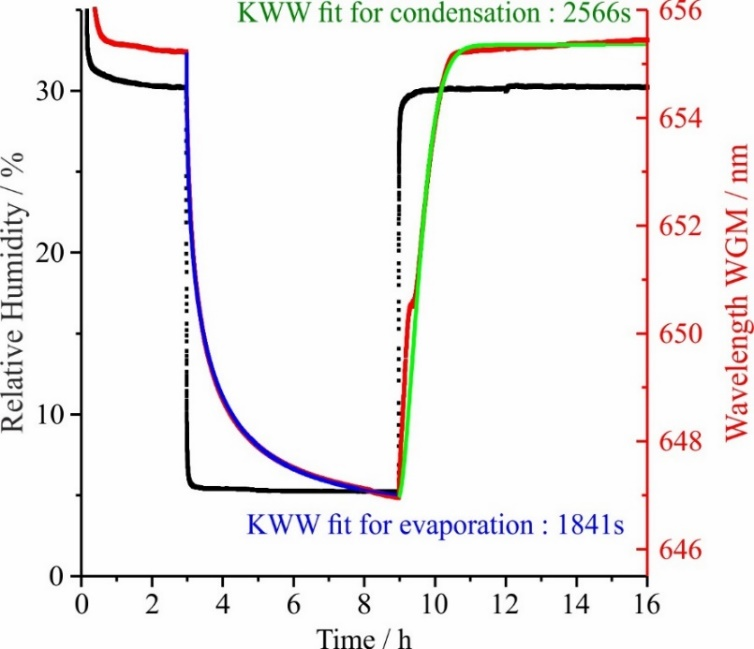
\includegraphics[width=0.8\textwidth]{chapters/water_hopping/figures/image003.jpg}
    \label{fig:wat_s1}
\end{figure}

\section{The Effect of Particle Size on Equilibration Time for Six Binary Organic Systems}
Before moving on to fit the compositional dependence of diffusion constants, we consider first the qualitative dependence on droplet size. The experiment conditions are divided into two main categories for evaporation and condensation in this study: a low viscosity transition (RH \SIrange{50}{30}{\percent} and RH \SIrange{30}{50}{\percent}) and a high viscosity transition (RH \SIrange{30}{5}{\percent} and RH \SIrange{5}{30}{\percent}). The six panels in figure \ref{fig:wat_s2} show measurements for six binary systems of aqueous-glucose, aqueous-sucrose, aqueous-trehalose, aqueous-raffinose, aqueous-maltose, and aqueous-levoglucosan. All measurements for the six binary organic mixtures clearly show different trends with respect to initial or final RH, but the characteristic timescale of water transport ($\tau$) clearly also shows a particle size dependence during evaporation or condensation.

\begin{figure}
    \centering
    \caption[Binary mixture response functions]{\textsc{Binary mixture response functions}. Examples of the response functions for size changes of six binary mixtures particles following a step change in RH}
    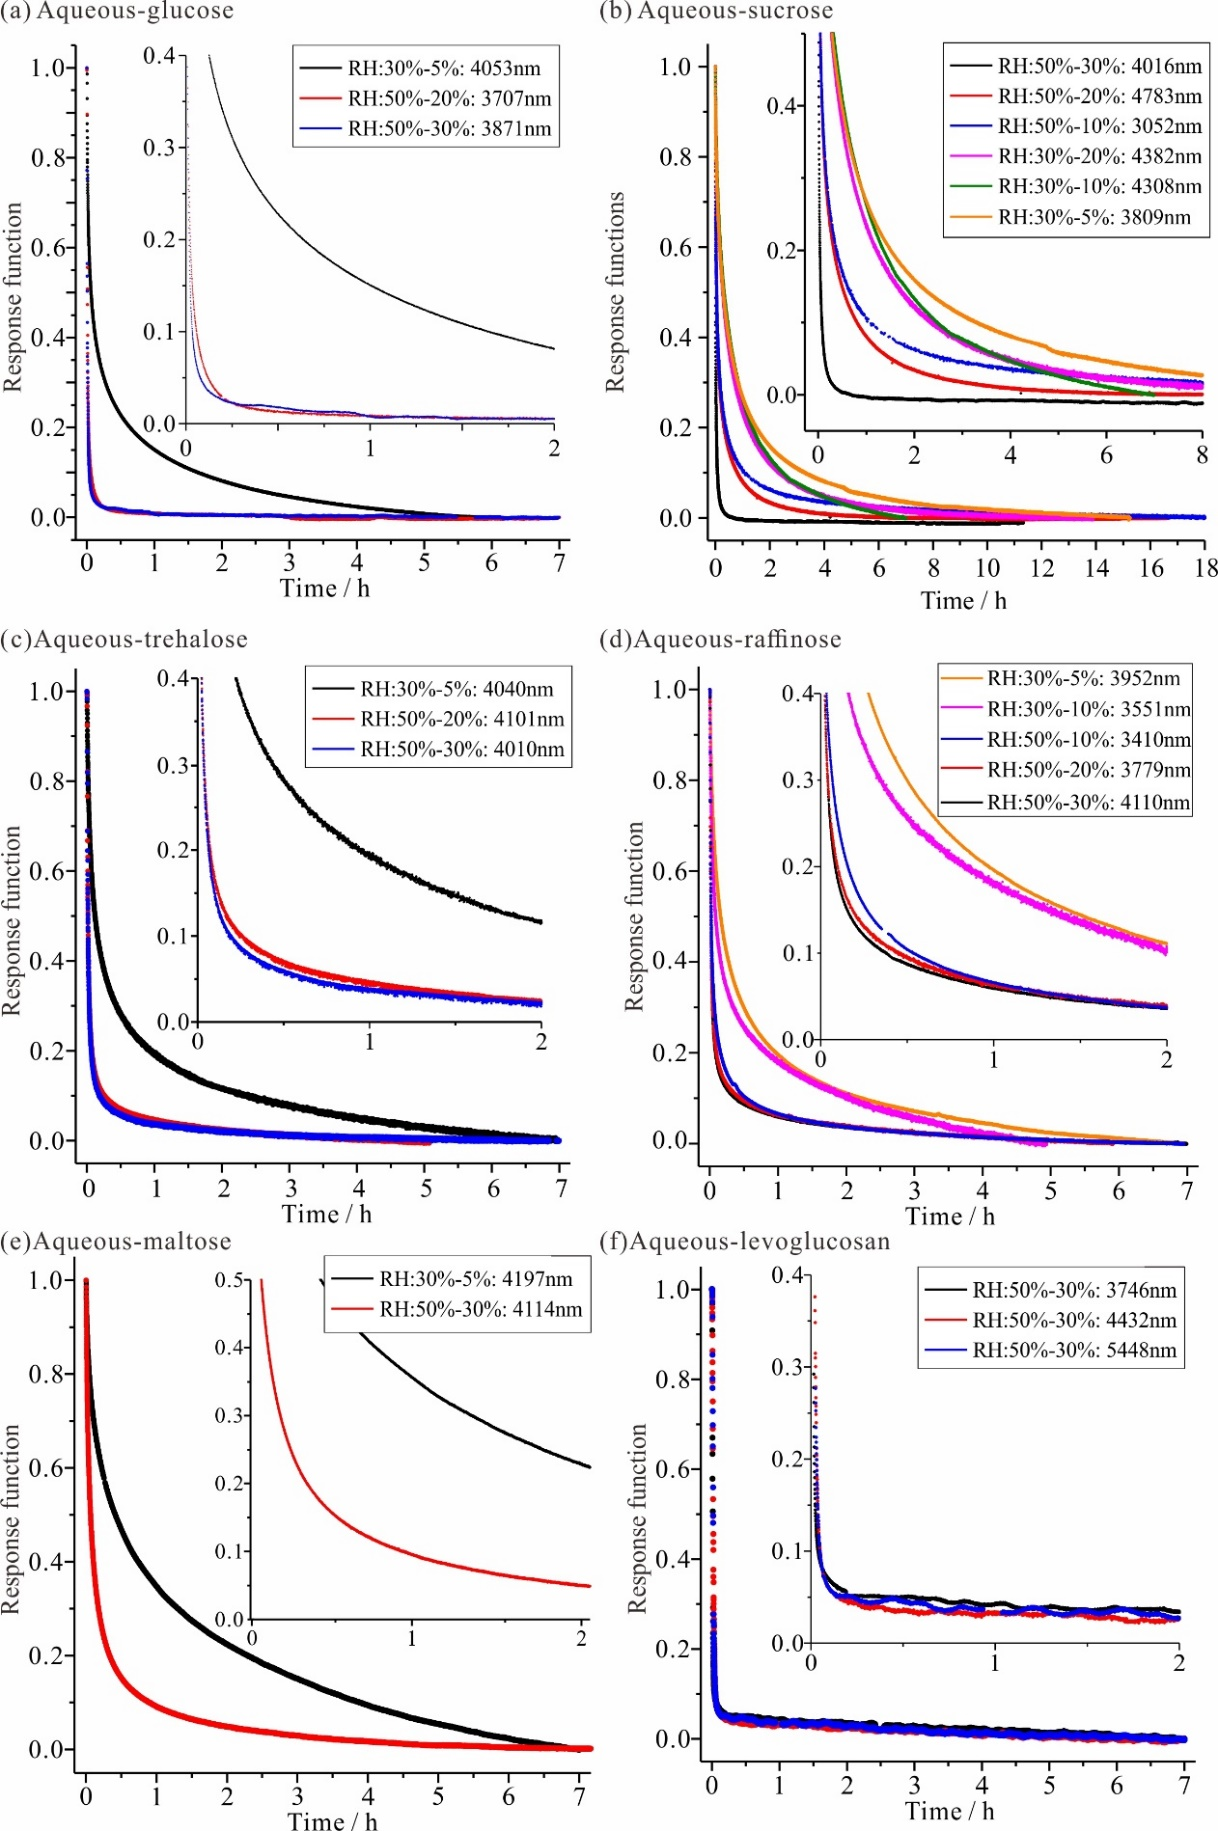
\includegraphics[width=0.8\textwidth]{chapters/water_hopping/figures/image004.jpg}
    \label{fig:wat_s2}
\end{figure}

In the high relative humidity region, transitions RH \SI{50}{\percent} - \SI{30}{\percent} - \SI{50}{\percent} (i.e., the evaporation step of RH \SI{50}{\percent} to \SI{30}{\percent} and condensation step of RH \SI{30}{\percent} to \SI{50}{\percent}), the droplets of maltose showed the largest value of timescale of water transport ($\tau$) over the other organic particles, see figure \ref{fig:wat_s3}. Moreover, the characteristic timescale increases with increasing particle size for every binary organic system. For example, the characteristic timescale of raffinose is \SI{188}{\second} for \SI{3332}{\nano\meter}, \SI{265}{\second} for \SI{4110}{\nano\meter}, and \SI{313}{\second} for \SI{4924}{\nano\second}. Comparing similarly sized particles of $\sim \SI{4}{\micro\meter}$ during an evaporation step, the organic particles show $\SI{514}{\second} \pm \SI{31}{\second}$ for maltose (\SI{4114}{\nano\meter}), $\SI{250}{\second} \pm \SI{23}{\second}$ for raffinose (\SI{3967}{\nano\meter}), $\SI{157}{\second} \pm \SI{13}{\nano\second}$ for trehalose (\SI{4101}{\nano\meter}), $\SI{59}{\nano\second} \pm \SI{19}{\second}$ for sucrose (\SI{4016}{\nano\meter}), $\SI{29}{\second} \pm \SI{3}{\second}$ for glucose (\SI{3871}{\nano\meter}), and $\SI{32}{\second} \pm \SI{4}{\second}$ for levoglucosan (\SI{3746}{\nano\meter}). The ordering of the timescales for all particles sizes in the range of \SIrange[range-phrase=--]{3}{6}{\micro\meter} show the same tendency: maltose $>$ raffinose $>$ trehalose $>$ sucrose $>$ glucose $\ge$ levoglucosan, as shown in figure \ref{fig:wat_s3}. In this region, raffinose and maltose particles have experienced the glass transition at RH $\sim \SI{53}{\percent}$ and RH $\sim\SI{32}{\percent}$ in the ambient temperature\cite{Song2016a,Tong2011}. However, trehalose, sucrose, glucose and levoglucosan do not pass through the glass transition RH until a much lower value. The molecular diffusivity of water in each organic system will be treated in the next section.

\begin{figure}
    \centering
    \caption[Timescale of water transport for evaporation step and condensation steps]{\textsc{Timescale of water transport ($\tau$) for evaporation step and condensation steps}. The values are also reported numerically in table \ref{tab:wat_s1}. The evaporation and condensation timescales are determined by KWW function, and particle size is calculated from the droplet Raman signal by the proprietary LARA software. Compositions are: (a) binary aqueous-glucose (b) binary aqueous-sucrose (c) binary aqueous-trehalose (d) binary aqueous-raffinose (e) binary aqueous-maltose (f) binary aqueous-levoglucosan}
    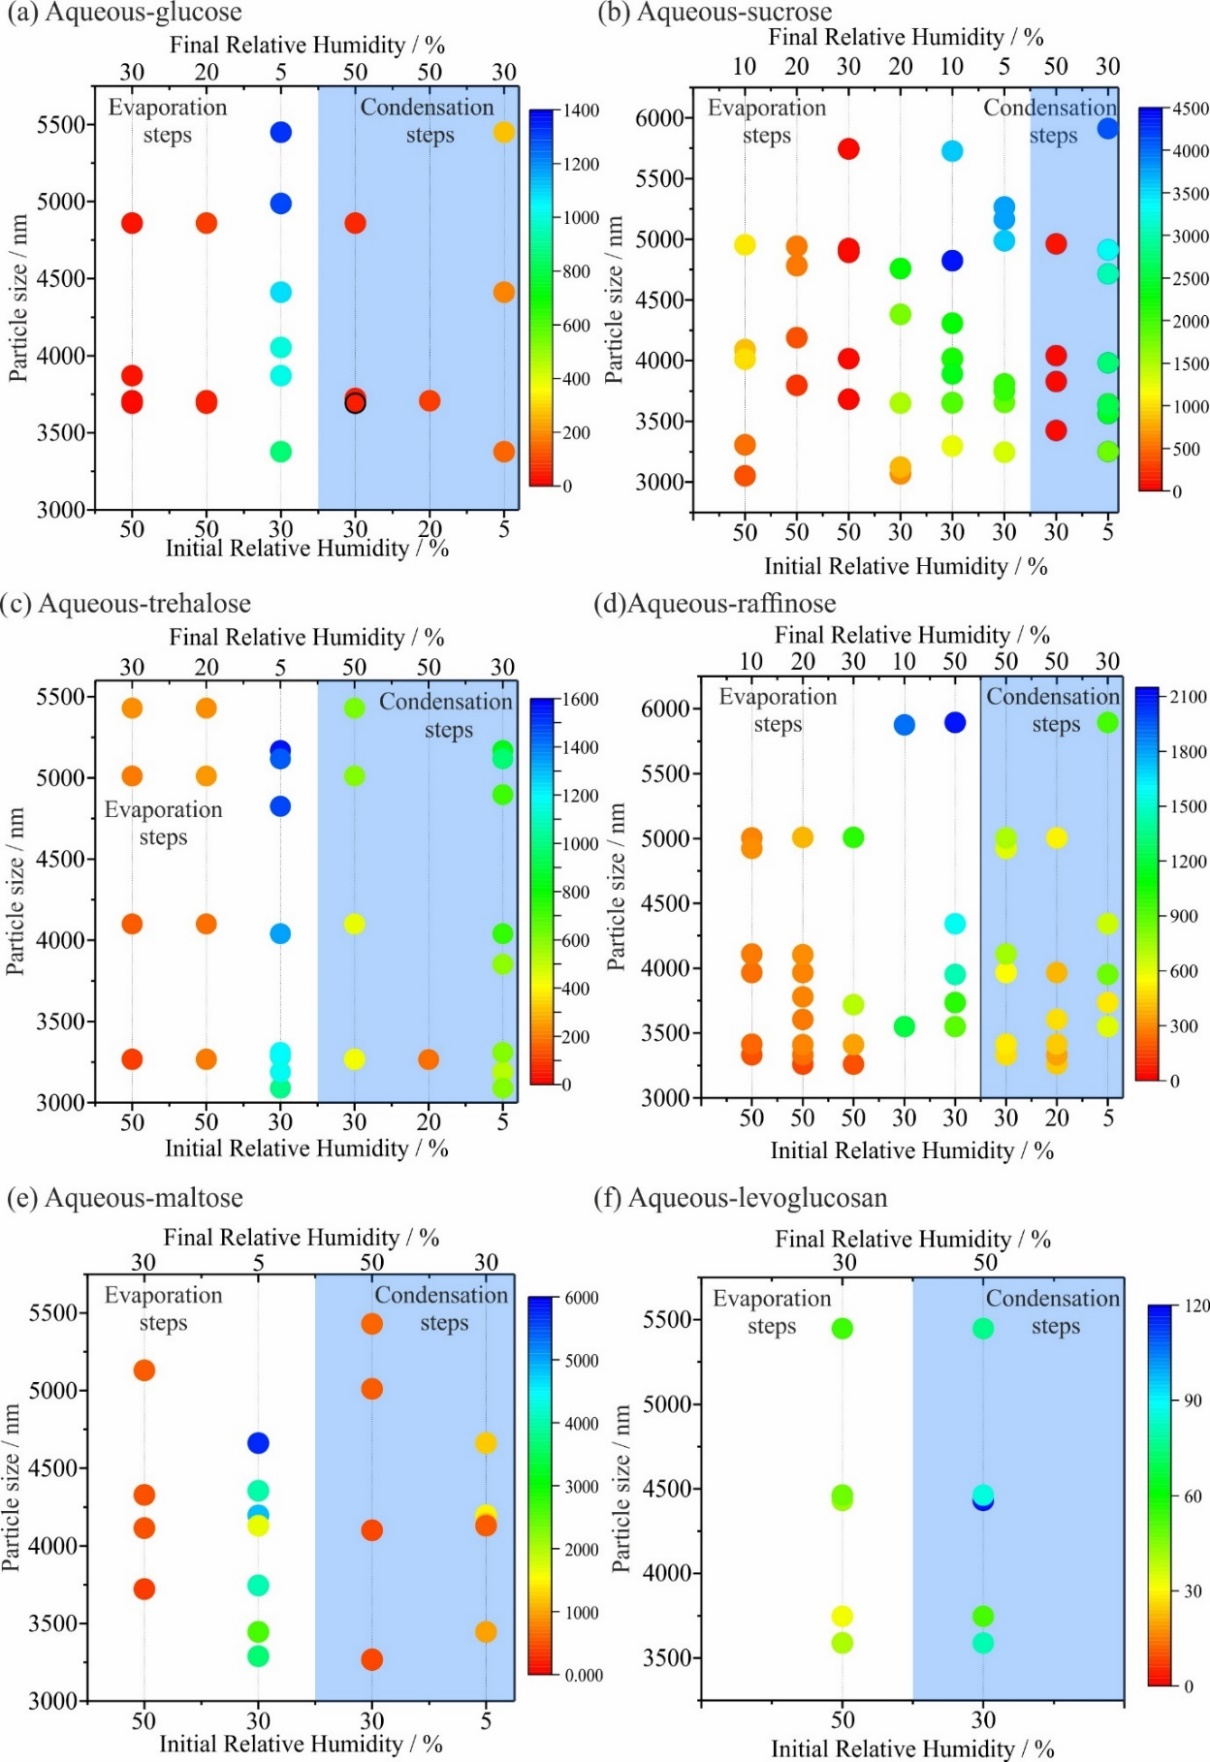
\includegraphics[width=0.8\textwidth]{chapters/water_hopping/figures/image005.jpg}
    \label{fig:wat_s3}
\end{figure}

For transitions at low relative humidity, notably for RH \SI{30}{\percent} to \SI{5}{\percent} and \SI{5}{\percent} to \SI{30}{\percent}, which is the high viscosity region for all compounds, the characteristic timescales of water transport of maltose particles have the longest water transport timescales in the low humidity region. Comparing similar sized particles of $\sim \SI{4}{\micro\meter}$ during an evaporation step, the organic particles showed the timescales as follows: $\SI{4062}{\second} \pm \SI{55}{\second}$ for maltose (\SI{3745}{\nano\meter}), $\SI{2035}{\second} \pm \SI{23}{\second}$ for sucrose (\SI{3809}{\nano\meter}), $\SI{1447}{\second} \pm \SI{19}{\second}$ for raffinose (\SI{3952}{\nano\meter}), $\SI{1342}{\second} \pm \SI{17}{\second}$ for trehalose (\SI{4040}{\nano\meter}), and $\SI{1009}{\second} \pm \SI{10}{second}$ for glucose (\SI{3871}{\nano\meter}). Levoglucosan cannot be measured in this RH region with particles crystallising at higher RH. The ordering of the timescales for all particles sized in the range of \SIrange[range-phrase=--]{3}{6}{\micro\meter} show the same tendency; maltose $>$ sucrose $>$ raffinose $>$ trehalose $>$ glucose, as shown in figure \ref{fig:wat_s2}. In this low RH region, raffinose (RH $\sim \SI{53}{\percent}$)\cite{Song2016a,Tong2011}, sucrose (RH $\sim \SI{23}{\percent}$)\cite{Song2016a,Tong2011}, trehalose (RH $\sim \SI{22}{\percent}$)\cite{Song2016a,chenLiteratureReviewSupplemented2000}, and maltose (RH $\sim \SI{32}{\percent}$)\cite{Song2016a,fosterGlassTransitionRelated2006} pass through the glass transition RH at ambient temperature except glucose, and glucose shows the smallest timescale for water transport. The characteristic timescale of water transport can be explained by water diffusion in the organic particles. All water transport experimental data go into Fi-PaD diffusion simulation.


\section{Equilibration Time variation with ``Wait Time'' Effect}
The relaxation dynamics for condensation processes are dependent on the ``wait time'' (i.e., also referred to the aging of the particle). Figure \ref{fig:wat_s4} shows the impact of ``wait time'' on the relaxation timescale of water transport in a binary water-sucrose system. In this case the relaxation timescale is the timescale for the re-condensation of water following a period of drying of varying time (the ``wait time''). Three different experimental conditions were studied. Sucrose particles that are indicated in black squares were dried for \num{5} hours at RH \SI{30}{\percent}, and then the particles were held at RH \SI{5}{\percent} for \num{6} hours. For comparison with this data set, sucrose droplets, indicated by red circles and blue triangles, were held at \num{12} and \num{24} hours at RH \SI{5}{\percent}. After \num{6}, \num{12}, and \num{24} hours at \SI{5}{\percent} RH, the RH is restored to the initial level \SI{30}{\percent} RH. Several sucrose particles across a range of particle size (\SIrange[range-phrase=--]{3}{5}{\micro\meter}) were studied at each RH transition. Figure \ref{fig:wat_s4} shows that when the particles experienced a long wait time, the relaxation timescale of water transport ($\tau$) increased during re-condensation following the increase in RH to the initial level. Depending on wait time under dry conditions, the water content varies both in magnitude and spatially before the RH is increased\cite{Rickards2015}. When increasing RH again, water vapor immediately condenses onto the particle surface, and leads to a unique level of heterogeneity which varies with the timescale over which moisture has been removed and the particle dried\cite{Rickards2015,luTimescalesWaterTransport2014}. The KWW equation was used to determine the timescales for the re-condensation step and the dependence on particle size is shown in the figure. When the particle size is larger, the timescale for re-condensation is also greater. The three trend lines in the figure, fitted by a linear equation, clearly indicate the relation between drying time, particle size and re-condensation timescale. The significance of the wait time is that when particle returned to the initial state from dry condition, the condensation time to return the particle to equilibrium with the surroundings increases as the wait time increases. 


\begin{figure}
    \centering
    \caption[Timescales of water transport]{\textsc{Timescales of water transport}. Timescale of water transport ($\tau$) for each condensation step of sucrose, RH change from \SI{30}{\percent} to \SI{5}{\percent} then back to \SI{30}{\percent} after drying. Particles of black squares experienced \num{6} hours drying time at RH \SI{5}{\percent}, particles of red circles experienced \num{12} hours drying time at RH \SI{5}{\percent}, and particles of blue triangles experienced \num{24} hours drying time at RH \SI{5}{\percent}. Error bars were calculated a variation of $\beta \pm \num{0.1}$.}
    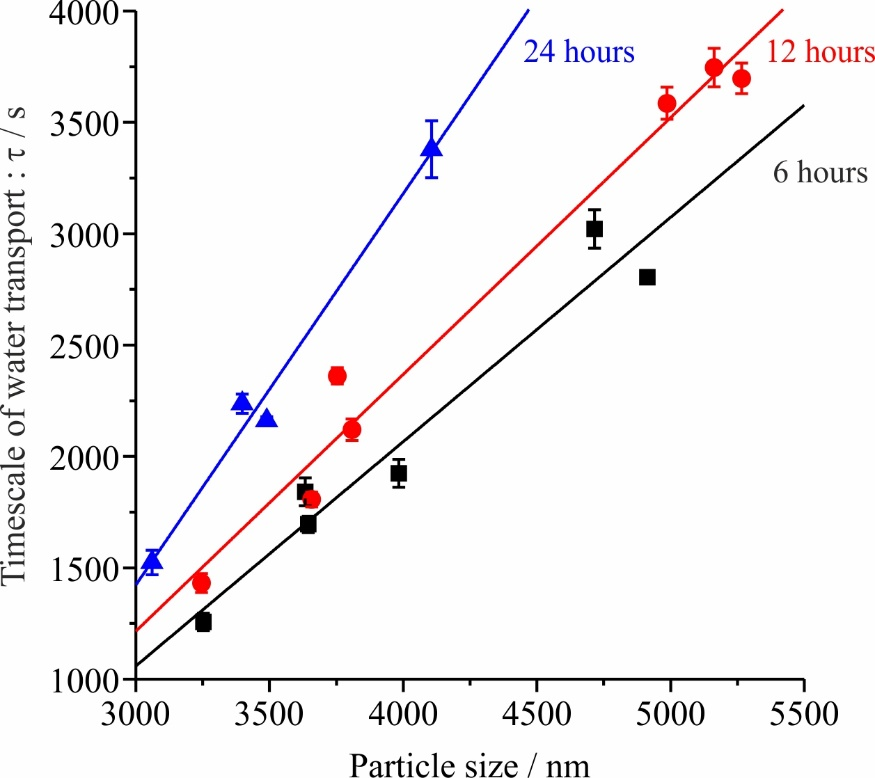
\includegraphics[width=0.8\textwidth]{chapters/water_hopping/figures/image006.jpg}
    \label{fig:wat_s4}
\end{figure}

\section{Fickian diffusion modelling (Fi-PaD model) for determining diffusivity of water in aerosol particles.}

In order to determine diffusivity of water in organic mixtures, a recently developed Fi-PaD model is applied to experimental data in this work. This was achieved using the same WGMs as were selected to fit KWW functions to.

O’Meara et al. developed a partial differential model, called Fi-PaD model, comparing it with two other diffusion models referred to as the ETH model and KM-GAP model (kinetic multi-layer model of gas-particle interactions in aerosol and clouds)\cite{omearaRateEquilibrationViscous2016}. The Fi-PaD model is established using Fick’s second law. The Fi-PaD model uses three initial assumptions below:
\begin{enumerate}
    \item An aerosol particle is spherical.
    \item A spherical particle is divided into inner concentric shells.
    \item A surface shell immediately reaches an equilibrium state with gas phase RH.
\end{enumerate}
According to these assumptions, an aerosol particle consists of a number of concentric shells within the particle bulk in the Fi-PaD model. In this thesis, the number of shells is \num{400} and the resolution of a shell is around \SI{10}{\nano\meter} for \SI{4}{\micro\meter} radii of particle. 

The Fi-PaD model is used to provide a forward simulation of the time-dependent size and response function following the step change in the gas phase RH change\cite{omearaRateEquilibrationViscous2016,Ingram2017}. A first guess for the water activity dependence of the diffusion coefficient is assumed. The diffusion coefficient of water in the mixture, $D_{w}$, is assumed to follow a Vignes form\cite{omearaRateEquilibrationViscous2016,Ingram2017}:
\begin{equation}\label{eqn:vignes_form}
D_{\mathrm{w}}(x, \alpha)=D_{\mathrm{w, w}}^{x \alpha} \times D_{\mathrm{w}, \mathrm{org}}^{(1-x \alpha)}
\end{equation}
where $x$ is the mole fraction of water, $D_{\mathrm{w, w}}$ is the known and limiting value of the diffusion coefficient of water in pure water, $D_{\mathrm{w}, \mathrm{org}}$ is diffusion coefficient of water in pure solute at infinite dilution of water. $\alpha$ is often viewed as analogous to an activity coefficient, given by:
\begin{equation}
\ln \alpha=A(1-x)^{3},
\end{equation}
where $A$ is a temperature dependent parameter. Using Fick’s second law, the model simulates the concentration change of every shell in the particle by calculating the approximate diffusional mass flux.  

All measurements are performed at room temperature ($\num{20}^{\circ}\mathrm{C}$). Thus, two fit parameters ($A$ and $D_{\mathrm{w,org}}$) are varied independently to achieve the best fit to the time-dependent size. For the example shown in figure \ref{fig:wat_f1} panel (a), the best-fit water activity dependence of the diffusion coefficient of water in the mixture is shown in figure \ref{fig:wat_f1} panel (b). 

\section{Holographic optical tweezers}
Holographic Optical Tweezers (HOT) are used to initiate the coalescence process between two aerosol particles and to, thereby, infer the particle viscosity at a particular gas phase RH/particle moisture content\cite{Song2016a}. In order to catch multiple droplets, the optical additional components are required and are shown in figure \ref{fig:wat_s5}. The most significant is the inclusion of a Spatial Light Modulator (Holoeye SLM LC-R 2500, twisted nematic, liquid crystal on silicon) on the right side and a high bit-rate oscilloscope (LeCroy Wavesurfer 454) with photo detector (Thorlabs DET 110) on the left side, as shown in figure \ref{fig:wat_s5}. The trapping beam is a continuous wave Nd:YVO4 laser at \SI{532}{\nano\meter} (maximum output is \SI{3}{\watt}, Opus, Laser Quantum). After the laser output, the trapping beam is a vertically polarised by a half-wave plate, and it directly passes through a telescope which adjusts beam size. The SLM is used to split the beam. A beam expansion telescope and inverted microscope objective generate the optical traps to capture aerosol particles. Using the half-wave plate, the power division between the SLM and a beam dump can be controlled. In the trapping cell, multiple droplets can be held by the split beam. During experimental measurements, particle images are recorded by camera, and Raman spectra are recorded by the spectrograph. Light scattering patterns following the initiation of coalescence event are recorded by the photo detector.

\begin{figure}
    \centering
    \caption[A schematic representation of Holographic Optical Tweezers (HOT)]{\textsc{A schematic representation of Holographic Optical Tweezers (HOT)}. The camera provides particle images, Raman spectrum is recorded by the spectrograph, and light scattering pattern is recorded by the photo detector\cite{Song2016a}.}
    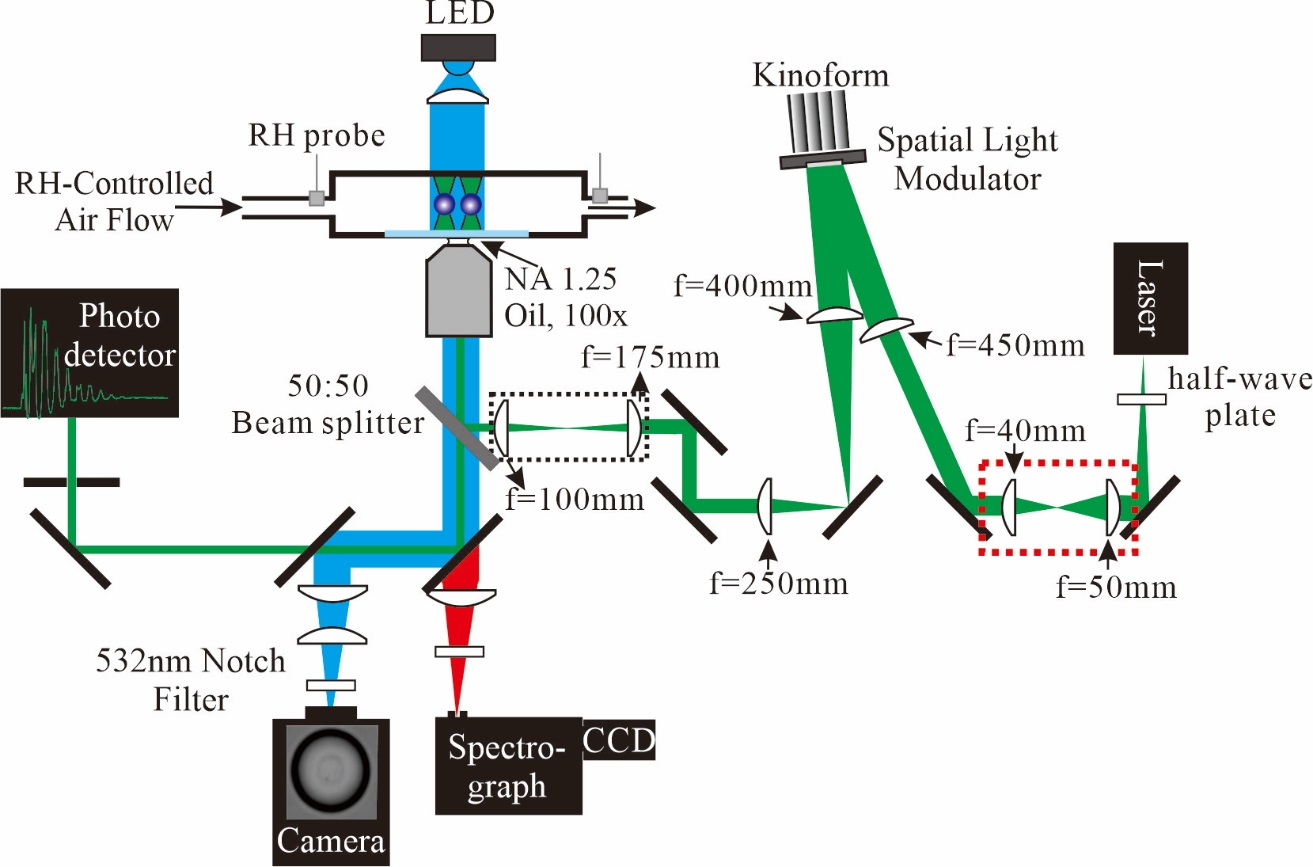
\includegraphics[width=0.8\textwidth]{chapters/water_hopping/figures/image011.jpg}
    \label{fig:wat_s5}
\end{figure}

\section{Viscosity of Saccharide Solutions Aerosol Particles}

Previously,the procedure for recording the viscosity of aerosols containing saccharides, alcohol, di- and tri-carboxylic acids  has been described, reporting viscosity measurements as a function of RH\cite{powerProbingMicrorheologicalProperties2014,Song2016a,powerTransitionLiquidSolidlike2013}. Briefly, pairs of aerosol particles of identical composition are captured in parallel optical traps formed using an holographic optical tweezers arrangement. The particles are conditioned at a fixed RH (in the range $<\SI{5}{\percent}$ to $>\SI{90}{\percent}$ RH) for a period of time that can extend to hours. It has been shown that this allows sufficient time for the particles to achieve a moisture content in equilibrium with the gas phase RH and a uniform homogeneous composition/viscosity\cite{Song2016a}. 

Coalescence is initiated by beam-steering, merging the pair of optical traps. At low viscosity ($<\SI{10}{\pascal\second}$), the particles may merge and relax in shape on a timescale less than \SI{1}{\milli\second}, a process that is monitored by measuring the relaxation in the back-scattered light from the optical trap. At higher viscosities, direct brightfield images can be recorded and the distortion in shape followed by determining the aspect ratio of the composite particle. The time-dependent decay in the aspect ratio can extend from milliseconds to $\gg \SI{10000}{\second}$, extending the viscosity range that can be measured from \SI{1}{\pascal\second}  up to \SIrange[range-phrase=--]{e8}{e9}{\pascal\second}\cite{Song2016a}. The viscosity is then inferred from the relaxation timescale, $\tau$, assuming over-damped creeping fluid flow, the droplet radius and an estimate of the surface tension, $\sigma$:
\begin{equation}
\tau=\frac{\eta r}{\sigma}
\end{equation}

A comparison of the viscosity trends for saccharides from mono- to tri- structures is provided in figure \ref{fig:wat_s6}. There is a clear systematic trend toward higher viscosity as the composition progresses from a monosaccharide to a trisaccharide, depending on chemical structure, and molecular weight, with an order: glucose (\SI{180.16}{\gram\per\mole}) $<$ sucrose (\SI{342.30}{\gram\per\mol}) $<$ trehalose (\SI{342.296}{\gram\per\mol}) $<$ maltose (\SI{342.30}{\gram\per\mol}) $<$ raffinose (\SI{504.42}{\gram\per\mol}).


\begin{figure}
    \centering
    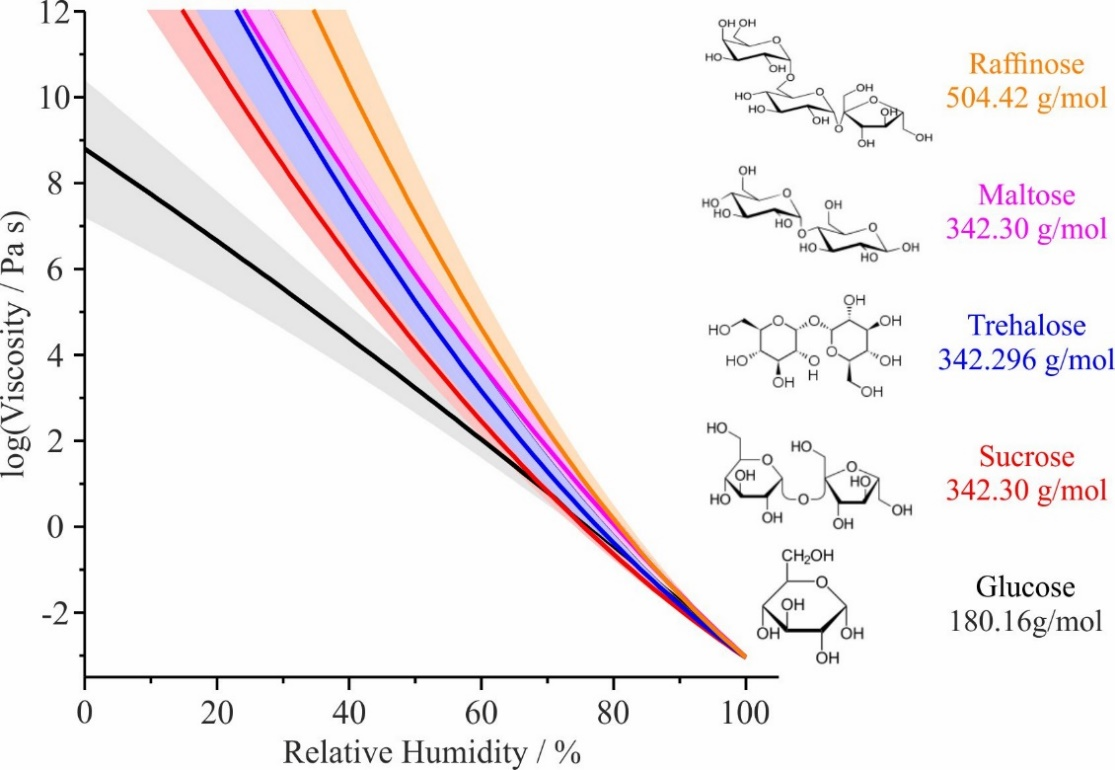
\includegraphics{chapters/water_hopping/figures/image014.jpg}
    \caption[A comparison of viscosity of different systems]{\textsc{A comparison of viscosity of different systems}. Aqueous glucose (black), aqueous sucrose (red) aqueous trehalose (blue), aqueous maltose (pink), and aqueous raffinose (orange)\cite{Song2016a}. Figure is redrawn from Song et. al.\cite{Song2016a}}
    \label{fig:wat_s6}
\end{figure}

\section{Molecular dynamics}
\subsection{Force Fields}
Water was represented by the TIP4P/2005\cite{abascalGeneralPurposeModel2005} potential, due to its accuracy in reproducing the experimental phase and self diffusion characteristics. Sucrose was represented by a modified version of the GROMOS 54a7 force field\cite{oostenbrinkBiomolecularForceField2004}, with an expanded range of atom types. Both the force field and the initial pdb all-atom coordinates were acquired from the automated topology builder (ATB) database\cite{koziaraTestingValidationAutomated2014} (further details on the generation\cite{maldeAutomatedForceField2011} and validation\cite{schmidDefinitionTestingGROMOS2011} of coordinates, partial charges and force fields by ATB has been detailed extensively in the literature).

Initial coordinates were generated using the Packmol\cite{martinez2009packmol} program, which randomly places set numbers of molecules into three dimensional space, allowing tight control over the solute mole fractions in the generated simulation boxes, whilst not biasing the simulations to one area of configuration space. Constraints were inserted such that no two molecules were placed within \SI{3}{\angstrom} of each other, and the input random seed was continuously replaced using the bash \texttt{\$RANDOM} global variable. 

The Lincs algorithm\cite{hess1997lincs} was used to constrain all bonds, to an order of four in the constraint coupling matrix, with seven iterations in the final step.Electrostatic forces were calculated using the particle mesh Ewald summation\cite{essmannSmoothParticleMesh1995}, and Van der Waals interactions were provided by the twin range cut-offs method, both of which were truncated at \SI{8}{\angstrom}. The update frequency was every \num{5} time-steps. The Verlet scheme\cite{pallFlexibleAlgorithmCalculating2013} was used for neighbour searching across the periodic boundary conditions in three dimensions. Velocities were generated using a Maxwell-Boltzmann distribution at \SI{300}{\kelvin}, with the random seed continuously changed.

\subsection{Equilibration}
 The starting coordinates produced by Packmol\cite{martinez2009packmol} are not suitable for MD simulations immediately. The configuration must be energy minimised using the steepest descent method to allow bonds and angles to satisfy the constraints of the topology file. The minimisation was conducted with an initial step size of \SI{0.001}{\nano\meter} until the maximum force was below \SI{50}{\kilo\joule\per\mole\per\nano\meter}. After this, approximately \SI{500}{\pico\second} of equilibration was conducted with the standard GROMACS MD integrator and thermodynamic ensemble produced as described in the main text. 

\subsection{Mean squared displacement data collection}
Initial coordinates were generated from the output frame of the equilibration trajectory within the regime where the total energy was stable. During the MD integration, the system was propagated in the NpT ensemble at \SI{300}{\kelvin} and \SI{101}{\kilo\pascal}, using a velocity rescaling thermostat\cite{bussiCanonicalSamplingVelocity2007} and the Parrinello-Rahman barostat\cite{parrinelloPolymorphicTransitionsSingle1981}, respectively. Initial velocities were randomly generated to satisfy a Maxwell-Boltzmann distribution at \SI{300}{\kelvin} in each case. All simulations described were conducted using GPU acceleration, with the MD package GROMACS (version 5.0.6)\cite{abrahamGROMACSHighPerformance2015}, running on the Blue Crystal 3 high performance computing cluster at the University of Bristol.

Due to the extremely kinetically limited state of the aqueous-sucrose system, it is necessary to simulate dynamics for very long periods of time, relative to, for example, the timescale of molecular vibration or rotation. This maximises the probability that the initial conditions are overcome, and that the constituent molecules decorrelated from their initial conditions as the simulation proceeds. In each of the trajectories of caged water, dynamics were computed for \SI{1}{\micro\second}, and it was found that, when averaged over all nine trajectories, the mean squared displacements of the water molecules converged to a diffusive dependence on simulation time, $t$ (figure \ref{fig:wat_s7}).
\begin{equation}\label{eqn:wat_msd}
\left\langle r^{2}\right\rangle=2 D_{\mathrm{w, org}} t
\end{equation}

The net displacement achieved by a random walk in three-dimensions will be less than the path length taken between the initial and final positions, a consequence of the fact that the translational motion of water through such a lattice is not Brownian. All nine trajectories contain segments during which the water is travelling perpendicularly, or even backwards, relative to its net displacement. It may be the case that the decorrelation of the water velocity is limited by the rearrangement of the sucrose, as well as the thermodynamic barrier that must be overcome to hop to the nearest available cavity, rather than the dynamics of a more typical solvation shell in an aqueous environment. Therefore, it is desirable to calculate the magnitude of the displacement to the current position, $\left|\left\langle r^{2}\right\rangle\right|$, at every time-step, rather than cumulatively sum the path length that takes into account every intermediate `jump’. Additionally, removal from the calculation of the centre of mass motion of the water molecule ensures that any atomically resolved vibrational motion does not contribute to the calculation of net displacement. The value stated in the manuscript and illustrated in figure \ref{fig:wat_f1} panel (c) was calculated under these conditions. 

\begin{figure}
    \centering
    \caption[Single particle mean squared displacement]{\textsc{Single particle mean squared displacement}. Shown are the $\left\langle r^{2}\right\rangle$ of the nine trajectories (purple), along with best fit of the mean path (red) to equation \ref{eqn:wat_msd} (yellow, including constant at $t=0$)}
    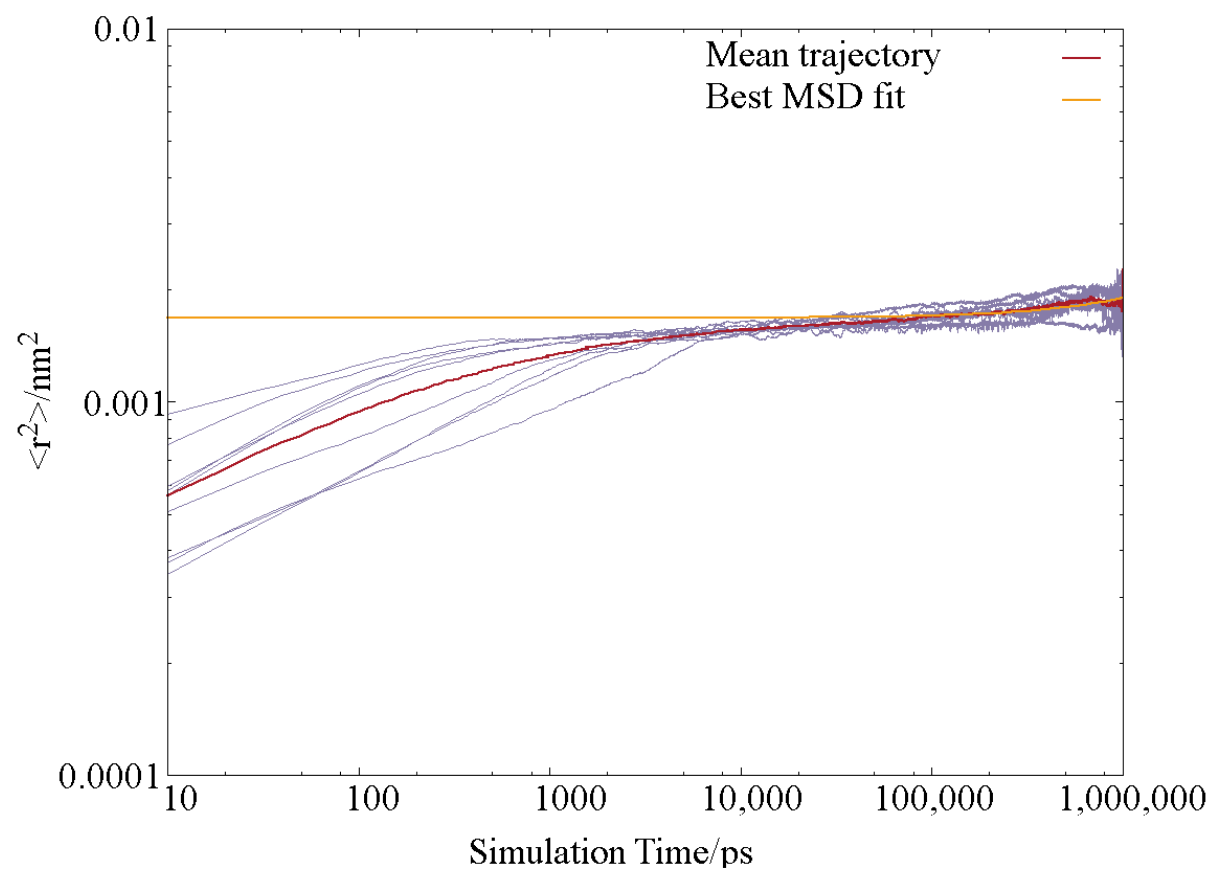
\includegraphics[width=0.8\textwidth]{chapters/water_hopping/figures/Fig_S7.png}
    \label{fig:wat_s7}
\end{figure}

These MD simulations were not designed to capture diffusion against a chemical potential gradient, which is what is induced and probed during the optical tweezers measurements reported above. Instead we wished to treat the water as a tracer particle moving stochastically through the matrix, subject to a small localization uncertainty arising from motion between adjacent frames\cite{michaletMeanSquareDisplacement2010}. This is the origin of the offset at $t=0$ in the figure. The per simulation $D$ values are presented in table \ref{tab:wat_s2}. 

A literature review was conducted to investigate whether any corrections or different functional forms of mean squared displacement needed to be fit. A recent publication\cite{alcazar-canoGeneralPhenomenologicalRelation2018} by Alcazar-Cano and Delgado-Buscalioni has suggested that in systems where the diffusing `tracer’ particles are trapped in the manner described here, and cannot freely move through channels, it may be more appropriate to fit $\left\langle r^{2}\right\rangle$ to a subdiffusive dependence, namely, 
\begin{equation}
\left\langle r^{2}\right\rangle \sim D_{\mathrm{w, org}} t^{\alpha}
\end{equation}
where $\alpha \rightarrow 0$ as the proportion of particles that are trapped approaches \SI{100}{\percent}. Similar physics was described by Zwanzig\cite{zwanzigDiffusionRoughPotential1988} earlier, in 1988, although it was incorporated into the mathematics by correcting $D$,rather than $t$. Specifically, Zwanzig considered a so-called `rough potential' where the particle under consideration must traverse a landscape of many nearly degenerate local minima. In that case, the observed $D$ is smaller than the effective $D$ by a factor $\epsilon$ that accounts for the `roughness' of the free energy landscape.

\begin{equation}
D_{\mathrm{w, org}}=D_{\mathrm{effective}} \exp \left(-\frac{\epsilon}{k T}\right)^{2}
\end{equation}

These  phenomena  are  often  observed  in  conjunction  with stretched  exponential  relaxation  in  sugar solutions\cite{mesteGlassTransitionFood2002,Liu2006}, which the radius curves in figure \ref{fig:wat_f1} panel (a) also exhibit. 

\subsection{Calculation free volume}
Three repeat trajectories of \SI{10}{\nano\second} length were conducted for glucose and raffinose, once again generated with randomly placed and oriented molecules via packmol and containing a single water. To determine the sucrose packing efficiency, truncated trajectories \SI{10}{\nano\second} long were extracted from the microsecond trajectories and subject to the same analysis, using the GROMACS `free-volume’ program, which attempts to insert `dummy’ probe particles into the box. The free volume calculated is the total volume of the successful insertions.

\section{Markov state modelling}

This section of the supplementary material has been incorporated into chapter \ref{chap:water}. 
\section{The comparison of diffusion coefficient of aqueous-sucrose system}

For diffusivity research, sucrose is a representative organic system because many researches have used sucrose. The comparison of diffusion curve of sucrose as a function of water activity is shown in figure \ref{fig:wat_s11}. The diffusion constants of water in aqueous-sucrose system in Figure S11 are measured and simulated with inferred by different strategies using AOT with Fi-Pad model, EDB with ETH model, and isotopic exchange. These three lines show good agreement until water activity \num{0.35}. The diffusion constants of water at \num{0.2} water activity by Price et al.\cite{Price2014} and this research differ by one order of magnitude. 

\begin{figure}
    \centering
    \caption[The diffusion curve of water in a sucrose system as a function of water activity]{\textsc{The diffusion curve of water in a sucrose system as a function of water activity}. The green line is from Zobrist et al.\cite{C0CP01273D}, the blue line from Price et al.\cite{Price2014}, and the red line is the experimental data which is simulated by Fi-PaD model.}
    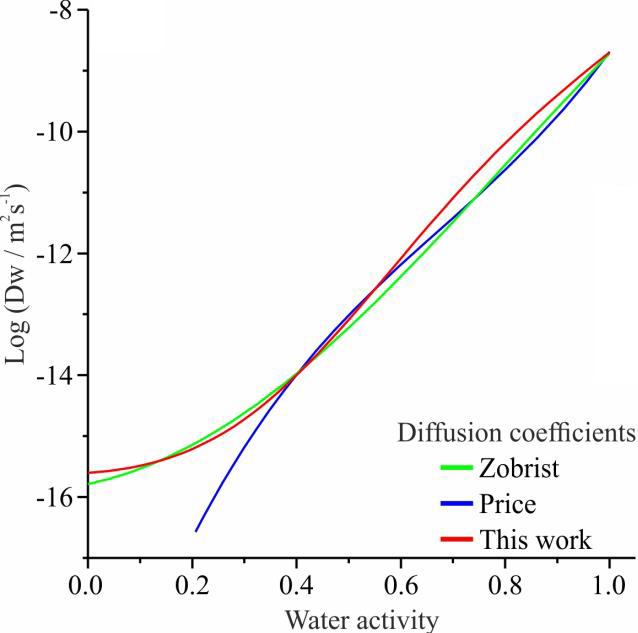
\includegraphics[width=0.8\textwidth]{chapters/water_hopping/figures/image058.png}
    \label{fig:wat_s11}
\end{figure}

\begin{xltabular}{0.9\textwidth}{YYYYYY}
    \caption[The characteristic timescale of water transport determined experimentally for six binary mixtures]{\textsc{The characteristic timescale of water transport determined experimentally for six binary mixtures}. This table provides all data points for water transport kinetics in figure \ref{fig:wat_s2}. Particle size is direct measurement data in AOT and fit by LARA. The characteristic timescale is fit by KWW function. Error representing a variation of $\beta \pm 0.1.$} \label{tab:wat_s1} \\
    \toprule 
    RH transition (\si{\percent}) & Particle size (\si{\nano\meter}) & Character-istic timescale (\si{\second})  & RH transition (\si{\percent}) & Particle size (\si{\nano\meter}) & Character-istic timescale (\si{\second}) \\ 
    \midrule
\endfirsthead
    \toprule
    \multicolumn{6}{c}{\tablename\ \thetable{} -- continued from previous page} \\
    RH transition (\si{\percent}) & Particle size (\si{\nano\meter}) & Character-istic timescale (\si{\second})  & RH transition (\si{\percent}) & Particle size (\si{\nano\meter}) & Character-istic timescale (\si{\second}) \\ 
    \midrule 
\endhead
    \midrule
    \multicolumn{6}{r}{{Continued on next page}} \\ 
    \bottomrule
\endfoot
\endlastfoot

    \multicolumn{3}{c}{\textbf{Aqueous-Glucose system}} & \multicolumn{3}{c}{\textbf{Aqueous-Maltose system}} \\
    
    50-30 &	3707 &	27	& 50-30	& 368 & 3721 \\
    -- & 	3692	& 27	& --& 	514	& 4114\\
    -- &  	3871	& 29	& --& 	534	& 4329 \\
    -- &  	4861	& 33	& --& 	549 & 5131 \\
    50-20 &	3707 &	49	& 30-5 &	3664 & 	3289 \\
    -- &  	3692	& 51	&-- & 	2624 & 	3446 \\
    -- &  	4861	& 92	&-- & 	4062 & 	3745 \\
    30-5 &	3377 &	860 & --&		4845	& 4197 \\
    --&  	4053 &	1007 & --& 		3996 & 	4355 \\
    --&  	3871 & 	1009 & --& 		5755 & 	4662 \\
    --&  	4412 & 	 1084 &-- & 		1641 & 	4130 \\
    --&  	4988 & 	1289 & 	30-50 &  	436 & 3265 \\
    --&  	5450 & 	1326 & --	& 	423	 & 3268 \\
    30-50	& 3707 & 	49 &-- & 		441 & 	4101 \\
    --&  	3692 & 	51	&-- & 	597 & 	5012 \\
    --&  	4861 & 	63 &-- & 		617	& 5430 \\
    20-50& 	3707 & 	95 & 5-30 & 	960	& 3446 \\
    5-30 & 	3377 & 	140	 &-- & 	1490	& 4197 \\
    --& 	4412 & 	190 & --& 		1250 & 	4662 \\
    --& 	5450 & 	276	&-- & 	1230 & 	4145 \\
    --& --	& --	&--&	578 & 	4130 \\
    \multicolumn{3}{c}{\textbf{Aqueous-Raffinose system}} & \multicolumn{3}{c}{\textbf{Aqueous-Sucrose system}} \\
    50-30 & 3332 & 188 & 50-10 & 3052 & 397 \\
    -- & 3414 & 221 & -- & 3307 & 535 \\
    -- & 3967 & 250 & -- & 4092 & 883 \\
    -- & 4110 & 265 & -- & 4013 & 1019 \\
    -- & 5005 & 298 & -- & 4954 & 1076\\
    -- & 4924 & 313 & 50-20 & 3796 & 244\\
    50-20 & 3260 & 153 & -- & 4189 & 363\\
    -- & 3332 & 254 & -- & 4783 & 540\\
    -- & 3410 & 288 & -- & 4942 & 559\\
    -- & 3966 & 284 & 50-30 & 3682 & 48\\
    -- & 3606 & 260 & -- & 4016 & 59\\
    -- & 3779 & 300 & -- & 4894 & 65\\
    -- & 4105 & 320 & -- & 4923 & 60\\
    -- & 5008 & 390 & -- & 5745 & 85\\
    50-10 & 3260 & 178 & 30-20 & 3068 & 668\\
    -- & 3410 & 352 & -- & 3123 & 847\\
    -- & 3719 & 700 & -- & 3651 & 1502\\
    -- & 5008 & 1010 & -- & 4382 & 1748\\
    30-10 & 3551 & 1210 & -- & 4758 & 2274\\
    -- & 5876 & 1906 & 30-10 & 3297 & 1243\\
    30-5 & 3551 & 895 & -- & 3654 & 1786\\
    -- & 3735 & 995 & -- & 3655 & 1901\\
    -- & 3952 & 1447 & -- & 3652 & 1924\\
    -- & 4343 & 1578 & -- & 4020 & 2141\\
    -- & 5895 & 2101 & -- & 4017 & 2191\\
    30-50 & 3332 & 482 & -- & 4308 & 2277\\
    -- & 3414 & 495 & -- & 3891 & 2379\\
    -- & 3967 & 547 & -- & 5727 & 3582\\
    -- & 4110 & 738 & -- & 4824 & 4374\\
    -- & 4924 & 617 & 30-5 & 3246 & 1321\\
    -- & 5005 & 730 & -- & 3657 & 1804\\
    20-50 & 3262 & 432 & -- & 3809 & 2035\\
    -- & 3332 & 351 & -- & 3754 & 2061\\
    -- & 3414 & 440 & -- & 4987 & 3584\\
    -- & 3606 & 476 & -- & 5163 & 3738\\
    -- & 3967 & 399 & -- & 5266 & 3763\\
    -- & 5005 & 516 & 30-50 & 3426 & 57\\
    5-30 & 3551 & 610 & -- & 3829 & 77\\
    -- & 3735 & 514 & -- & 4042 & 79\\
    -- & 3952 & 852 & -- & 4962 & 112\\
    -- & 4343 & 646 & 5-30 & 3252 & 1776\\
    -- & 5895 & 926 & -- & 3645 & 2059\\
    -- & -- & -- & -- & 3563 & 2395\\
    -- & -- & -- & -- & 3633 & 2566\\
    -- & -- & -- & -- & 3983 & 2763\\
    -- & -- & -- & -- & 4716 & 3056\\
    -- & -- & -- & -- & 4912 & 3294\\
    -- & -- & -- & -- & 5912 & 4112\\
    
    \multicolumn{3}{c}{\textbf{Aqueous-Raffinose system}} & \multicolumn{3}{c}{\textbf{Aqueous-Sucrose system}} \\
    50-30 & 3265 & 98 & 50-30 & 3590 & 35 \\
    -- & 3268 & 101 & -- & 3588 & 40 \\
    -- & 4101 & 157 & -- & 3746 & 32 \\
    -- & 5430 & 231 & -- & 4432 & 43 \\
    -- & 5012 & 204 & -- & 4463 & 47 \\
    50-20 & 3265 & 221 & -- & 5448 & 53 \\
    -- & 3268 & 194 & 30-50 & 3588 & 81 \\
    -- & 4101 & 184 & -- & 3746 & 52 \\
    -- & 5012 & 244 & -- & 4432 & 117 \\
    -- & 5430 & 233 & -- & 4463 & 86 \\
    30-5 & 3090 & 1019 & -- & 5448 & 76 \\
    -- & 3190 & 1172 & -- & -- & -- \\
    -- & 3285 & 1155 & -- & -- & -- \\
    -- & 3310 & 1184 & -- & -- & -- \\
    -- & 4040 & 1342 & -- & -- & -- \\
    -- & 4825 & 1479 & -- & -- & -- \\
    -- & 5168 & 1559 & -- & -- & -- \\
    -- & 5118 & 1444 & -- & -- & -- \\
    30-50 & 3265 & 436 & -- & -- & -- \\
    -- & 3268 & 423 & -- & -- & -- \\
    -- & 4101 & 441 & -- & -- & -- \\
    -- & 5430 & 617 & -- & -- & -- \\
    -- & 5012 & 597 & -- & -- & -- \\
    20-50 & 3265 & 181 & -- & -- & -- \\
    5-30 & 4040 & 726 & -- & -- & -- \\
    -- & 3190 & 515 & -- & -- & -- \\
    -- & 3090 & 592 & -- & -- & -- \\
    -- & 5168 & 846 & -- & -- & -- \\
    -- & 3853 & 589 & -- & -- & -- \\
    -- & 4897 & 719 & -- & -- & -- \\
    -- & 5118 & 981 & -- & -- & -- \\
    -- & 3310 & 596 & -- & -- & -- \\
    \bottomrule
    
\end{xltabular}

\begin{table}
    \centering
    \caption[Diffusion constants from MD trajectories]{\textsc{Diffusion constants from MD trajectories}. The best fit diffusion coefficients to the nine \SI{1}{\micro\second} trajectories (purple lines in figure \ref{fig:wat_s7}) and associated uncertainties.}
    \begin{tabular}{lrr}
    \toprule
    Trajectory no. & $D$ (\si{\meter\squared\per\second}) & Uncertainty  (\si{\meter\squared\per\second})  \\
    \midrule
    1 &	6.454E-17	& 9.34E-17 \\
    2 &	4.848E-17	& 1.755E-16 \\
    3 &	6.075E-17	& 1.444E-16 \\
    4 &	8.922E-18	& 3.448E-17 \\
    5 &	1.004E-18	& 1.88E-16 \\
    6 &	8.775E-17	& 2.218E-17 \\
    7 &	3.541E-17	& 8.571E-17 \\
    8 &	3.829E-17	& 1.61E-17 \\
    9 &	7.269E-17	& 5.83E-17 \\
    \bottomrule
    \end{tabular}
    \label{tab:wat_s2}
\end{table}

\begin{table}
    \centering
    \caption[Six binary system diffusion coefficients]{\textsc{Six binary system diffusion coefficients}. The best fit diffusion coefficients of six binary systems in figure \ref{fig:wat_f1} panel (c).}
    \begin{tabularx}{\textwidth}{p{3cm}X}
    \toprule
    System & Paramaterization ($D_w(a_w)$ (\si{\meter\squared\per\second})) \\
    \midrule
        Aqueous-Levoglucosan &  
        \begin{minipage}[c]{\linewidth}
        \begin{multline*}
         \log \left(\mathrm{D}_{\mathrm{w}}\left(\mathrm{a}_{\mathrm{w}}\right)\right)=-14.091+\left(2.192 \times \mathrm{a}_{\mathrm{w}}\right)\\
         +\left(-21.269\times\left(\mathrm{a}_{\mathrm{w}}\right)^{2}\right)+\left(81.025 \times\left(\mathrm{a}_{\mathrm{w}}\right)^{3}\right)\\
         +\left(-84.660 \times\left(\mathrm{a}_{\mathrm{w}}\right)^{4}\right)+\left(28.081\times\left(\mathrm{a}_{\mathrm{w}}\right)^{5}\right)      
        \end{multline*}
        \end{minipage} \\
        \midrule
        Aqueous-glucose &  
        \begin{minipage}[c]{\linewidth}
        \begin{multline*}
         \log \left(\mathrm{D}_{\mathrm{w}}\left(\mathrm{a}_{\mathrm{w}}\right)\right)=-15.047 +\left(0.963  \times \mathrm{a}_{\mathrm{w}}\right)\\
         +\left(-0.186 \times\left(\mathrm{a}_{\mathrm{w}}\right)^{2}\right)+\left(34.825 \times\left(\mathrm{a}_{\mathrm{w}}\right)^{3}\right)\\
         +\left(-47.724 \times\left(\mathrm{a}_{\mathrm{w}}\right)^{4}\right)+\left(18.472\times\left(\mathrm{a}_{\mathrm{w}}\right)^{5}\right)      
        \end{multline*}
        \end{minipage} \\
        \midrule
        Aqueous-sucrose &  
        \begin{minipage}[c]{\linewidth}
        \begin{multline*}
         \log \left(\mathrm{D}_{\mathrm{w}}\left(\mathrm{a}_{\mathrm{w}}\right)\right)=-15.613  +\left(1.262  \times \mathrm{a}_{\mathrm{w}}\right)\\
         +\left(-3.476 \times\left(\mathrm{a}_{\mathrm{w}}\right)^{2}\right)+\left(46.468 \times\left(\mathrm{a}_{\mathrm{w}}\right)^{3}\right)\\
         +\left(-60.030 \times\left(\mathrm{a}_{\mathrm{w}}\right)^{4}\right)+\left(22.691\times\left(\mathrm{a}_{\mathrm{w}}\right)^{5}\right)      
        \end{multline*}
        \end{minipage} \\
        \midrule
        Aqueous-Trehalose &  
        \begin{minipage}[c]{\linewidth}
        \begin{multline*}
         \log \left(\mathrm{D}_{\mathrm{w}}\left(\mathrm{a}_{\mathrm{w}}\right)\right)=-15.503   +\left(1.061  \times \mathrm{a}_{\mathrm{w}}\right)\\
         +\left(0.642 \times\left(\mathrm{a}_{\mathrm{w}}\right)^{2}\right)+\left(34.712  \times\left(\mathrm{a}_{\mathrm{w}}\right)^{3}\right)\\
         +\left(-48.590 \times\left(\mathrm{a}_{\mathrm{w}}\right)^{4}\right)+\left(18.981\times\left(\mathrm{a}_{\mathrm{w}}\right)^{5}\right)      
        \end{multline*}
        \end{minipage} \\
        \midrule
        Aqueous-Maltose &  
        \begin{minipage}[c]{\linewidth}
        \begin{multline*}
         \log \left(\mathrm{D}_{\mathrm{w}}\left(\mathrm{a}_{\mathrm{w}}\right)\right)=-15.857   +\left(1.269  \times \mathrm{a}_{\mathrm{w}}\right)\\
         +\left(-6.922  \times\left(\mathrm{a}_{\mathrm{w}}\right)^{2}\right)+\left(58.525  \times\left(\mathrm{a}_{\mathrm{w}}\right)^{3}\right)\\
         +\left(-72.854 \times\left(\mathrm{a}_{\mathrm{w}}\right)^{4}\right)+\left(27.141\times\left(\mathrm{a}_{\mathrm{w}}\right)^{5}\right)       
        \end{multline*}
        \end{minipage} \\
        \midrule
        Aqueous-Raffinose &  
        \begin{minipage}[c]{\linewidth}
        \begin{multline*}
         \log \left(\mathrm{D}_{\mathrm{w}}\left(\mathrm{a}_{\mathrm{w}}\right)\right)=-15.393   +\left(1.113  \times \mathrm{a}_{\mathrm{w}}\right)\\
         +\left(2.180  \times\left(\mathrm{a}_{\mathrm{w}}\right)^{2}\right)+\left(29.194   \times\left(\mathrm{a}_{\mathrm{w}}\right)^{3}\right)\\
         +\left(-42.838 \times\left(\mathrm{a}_{\mathrm{w}}\right)^{4}\right)+\left(17.051\times\left(\mathrm{a}_{\mathrm{w}}\right)^{5}\right)      
        \end{multline*}
        \end{minipage} \\
        \bottomrule
    \end{tabularx}
    \label{tab:wat_s3}
\end{table}

\chapter{Markov state model optimisation}\label{app:msm}

\begin{table}[h]
 \centering
 \caption[Gaussian process model selection metrics of the response surface of alanine dipeptide]{\textsc{Gaussian process model selection metrics of the response surface of alanine dipeptide}. Standardised mean square error (SMSE) and mean standardised log loss (MSLL) for GP models of the response surface of MSMs for alanine dipeptide, using different transformations of $n$ ($T(n)$) and different kernels. Each GP model used a mean prior of zero, and all other parameters were estimated by maximizing the marginal likelihood. All values were calculated using 10-fold cross-validation.}
 \begin{tabular}{lllrr}
 \toprule
 T(n) & Name & SMSE & MSLL \\
 \midrule
 $\log{(n)}$ & Exponential & 0.0012 & -3.9963 \\
 & Mat{\'e}rn 3-2 & 0.0010 & -4.1712 \\
 & Mat{\'e}rn 5-2 & 0.0007 & -4.2369 \\
 & Gaussian & 0.0011 & -4.0892 \\
 $I(n)$ & Exponential & 0.0027 & -2.9733 \\
 & Mat{\'e}rn 3-2 & 0.0025 & -3.4218 \\
 & Mat{\'e}rn 5-2 & 0.0023 & -3.8172 \\
 & Gaussian & 0.0032 & -4.1239 \\
 \bottomrule
 \end{tabular}
 \label{tab:ala2_fit_results}
\end{table}

\chapter{Metastable state selection for hidden Markov models}\label{app:hmm}

\section{Prinz potential}

 The Prinz potential is given by: 
\begin{equation}\label{eqn:prinz_pot}
 V(x) = 4\left(x^8 + 0.8 \exp{\left(-80 x^2\right)} + 0.2 \exp{\left(-80 (x-0.5)^2\right)} + 0.5\exp{\left(-40 (x+0.5)^2\right)}\right).
\end{equation}
Exact eigenvalues and trajectories of simulated Brownian motion were calculated using code from MSMBuilder (version 3.9.0)\cite{beauchampMSMBuilder2ModelingConformational2011} . The first $7$ relaxation processes are given in table \ref{tab:prinz_its_exact}. 
\begin{table}
 \centering
 \caption[Relaxation timescales of the Prinz potential]{\textsc{Relaxation timescales of the Prinz potential}. All values are given in units of the time step $\Delta t = 0.001$}
 \begin{tabular}{lr}
 \toprule
 Process, $i$ & $t_i$ \\
 \midrule
  2 & 844.4 \\
  3 & 125.5 \\
  4 & 64.3 \\
  5 & 11.9 \\
  6 & 10.3 \\
  7 & 7.3 \\
  8 & 6.7 \\
  \bottomrule
 \end{tabular}
 \label{tab:prinz_its_exact}
\end{table}

\num{100} trajectories of Brownian dynamics were simulated by the following stochastic differential equation: 
\begin{equation}\label{eqn:prinz_dynamics}
 \frac{\mathrm{d}x_t}{\mathrm{d}t} = -\frac{\mathrm{d}V(x)}{\mathrm{d}x} + \sqrt{2D}\cdot R(t)
\end{equation}
with $D = 1000$, and $R\sim \mathcal{N}(0, 1)$, $\mathrm{Cov}\left[R(t), R(t^{\prime})\right]=\delta_{t, t^{\prime}}$. The time-step used was $\Delta t = 0.001$. Each trajectory was initiated from a random draw of the stationary distribution and was twice the longest relaxation process timescale, i.e. $2\times 844=1688$ time-steps long. The trajectories were clustered into $n = \left\lfloor\sqrt{100\times 1688}\right\rfloor =410$ discrete states using k-means clustering\cite{friedman2001elements}. This number of states was based on the heuristic described in reference \cite{husicWardClusteringImproves2017a}.

\section{Membership matrix errors}\label{sec:app_membership_errors}

The conditional probabilities $\mathbb{P}(h=j|s=i)$ can be calculated via the $\gamma$ auxiliary variable from the Baum-Welch algorithm\cite{baumMaximizationTechniqueOccurring1970, welch2003hidden}, or from the membership matrix after taking into account the largest strongly connected subset of hidden states.  Figure \ref{fig:membership_error} shows the difference between these two methods for a HMM with $g=10$ hidden states.  The error plotted in panel (a) (blue discs) is given by:
\begin{equation}\label{eqn:err_entropy}
\mathrm{err}(s_{i}) = \sum_j\bar{\gamma}_{j}(s_{i}) - M_{i, j}, 
\end{equation}
and is plotted as a function of the stationary distribution of the observed states $\pi_{s_{i}}$. The green discs are the stationary distribution of states with zero error ($\mathrm{err}<10^{-10}$). $\bar{\gamma}$ is the value of $\gamma_{j}(s_{i})$ averaged over all the instances of a $s_{i}$ in a trajectory. As the size of the error decreases with frequency of the observed state, it can be concluded that the difference between the two methods arises from sampling error. Panel (b) shows the value of the error for just one hidden state (state $j=3$) with the emission distribution for comparison. 
\begin{figure}
    \centering
    \caption[Errors in the membership matrix]{\textsc{Errors in the membership matrix}. Panel (a) shows the error from equation \ref{eqn:err_entropy} (blue discs) as a function of the observed stationary distribution, $\bm{\pi}_{\mathrm{obs}}$. The green discs show the observed states with no difference in value of $\gamma$ or $\mathbf{M}$. Panel (b) shows the error for hidden state $3$ (blue discs) overlaid on the value of $\gamma_{3}(s)$ as a function of $s$, the observed states.}
    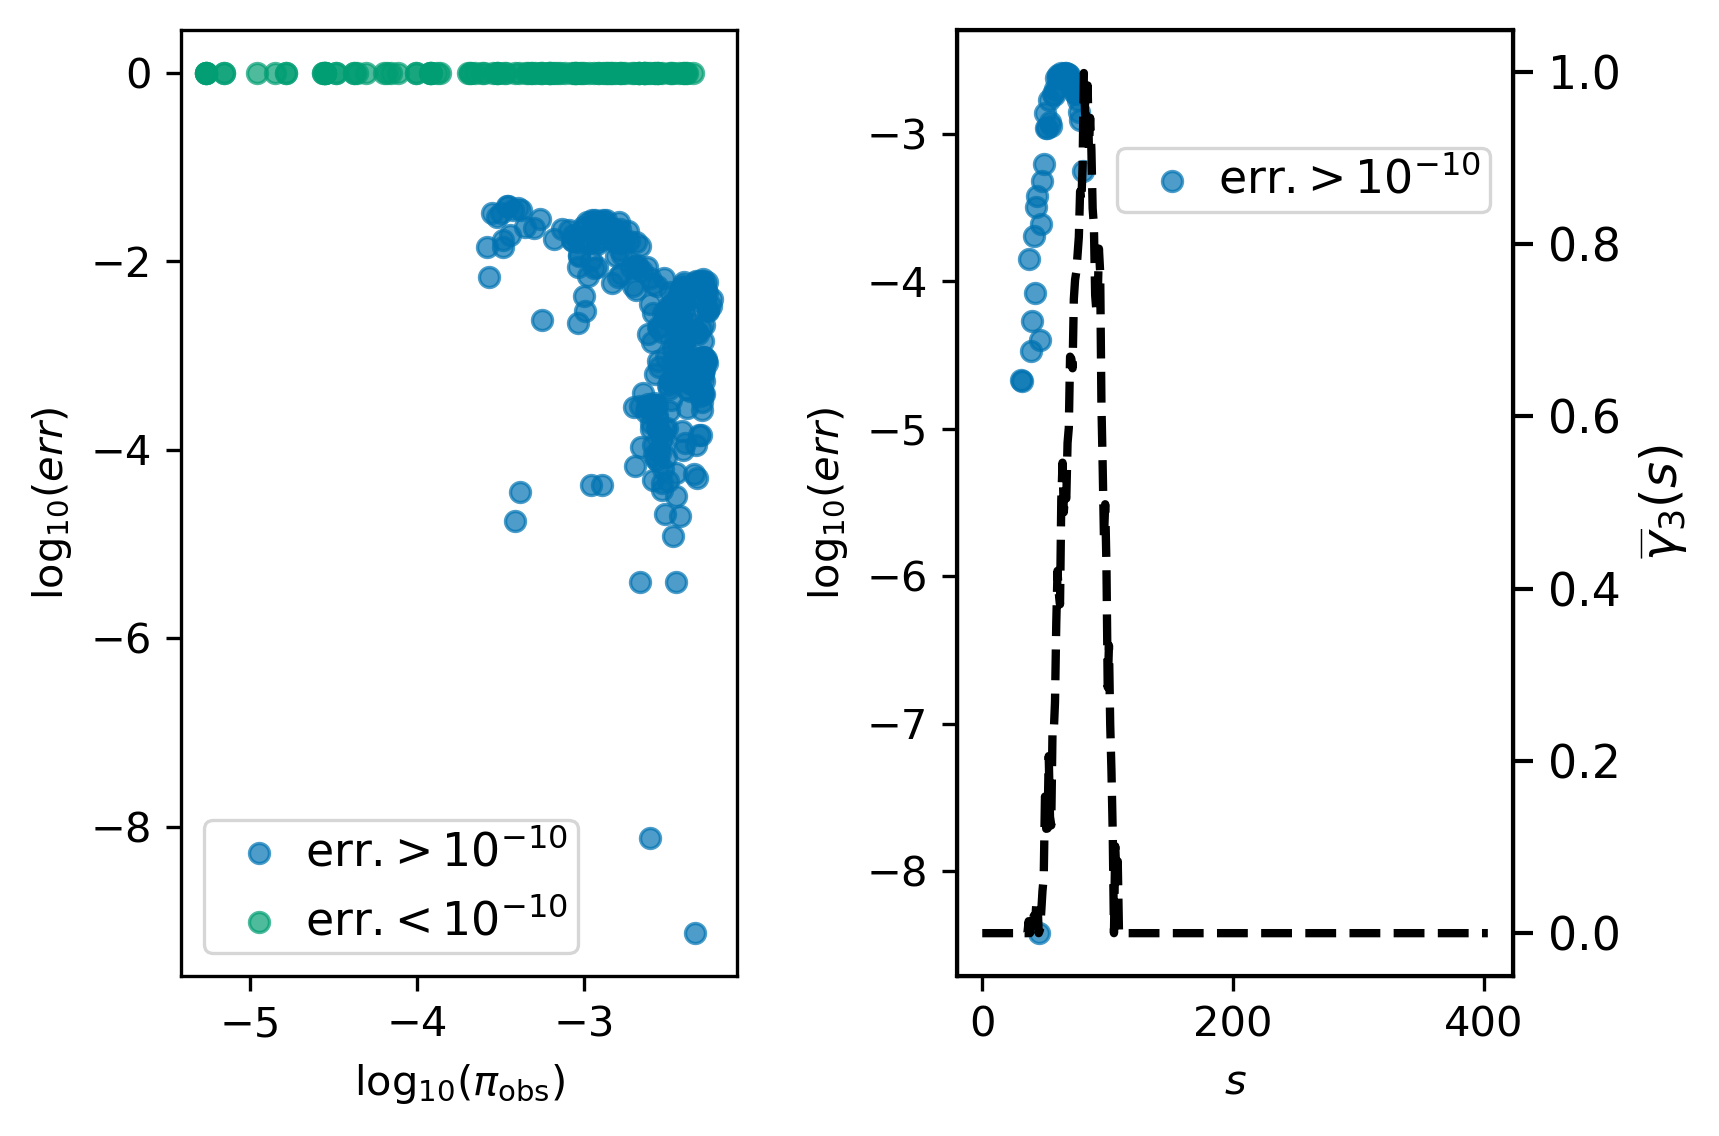
\includegraphics[width=0.8\textwidth]{chapters/hmm_selection/figures/entropy_error_explanation.png}
    \label{fig:membership_error}
\end{figure}

\chapter{Aromatic amine dehyrogenase}\label{app:aadh}

% \section{Molecular dynamics}

\begin{figure}[ph!]
 \centering
 \caption[RMSD of the alpha-carbon atoms of AADH relative to the crystal structure]{\textsc{RMSD of the $\alpha$-carbon atoms of AADH relative to the crystal structure}. Each panel is a single trajectory, blue lines are the RMSD, horizontal lines are the \SI{2.5}{\percent} and \SI{97.5}{\percent} quantiles (\SI{4.5}{\angstrom} and \SI{6.4}{\angstrom}, respectively) taken across all trajectories.}
 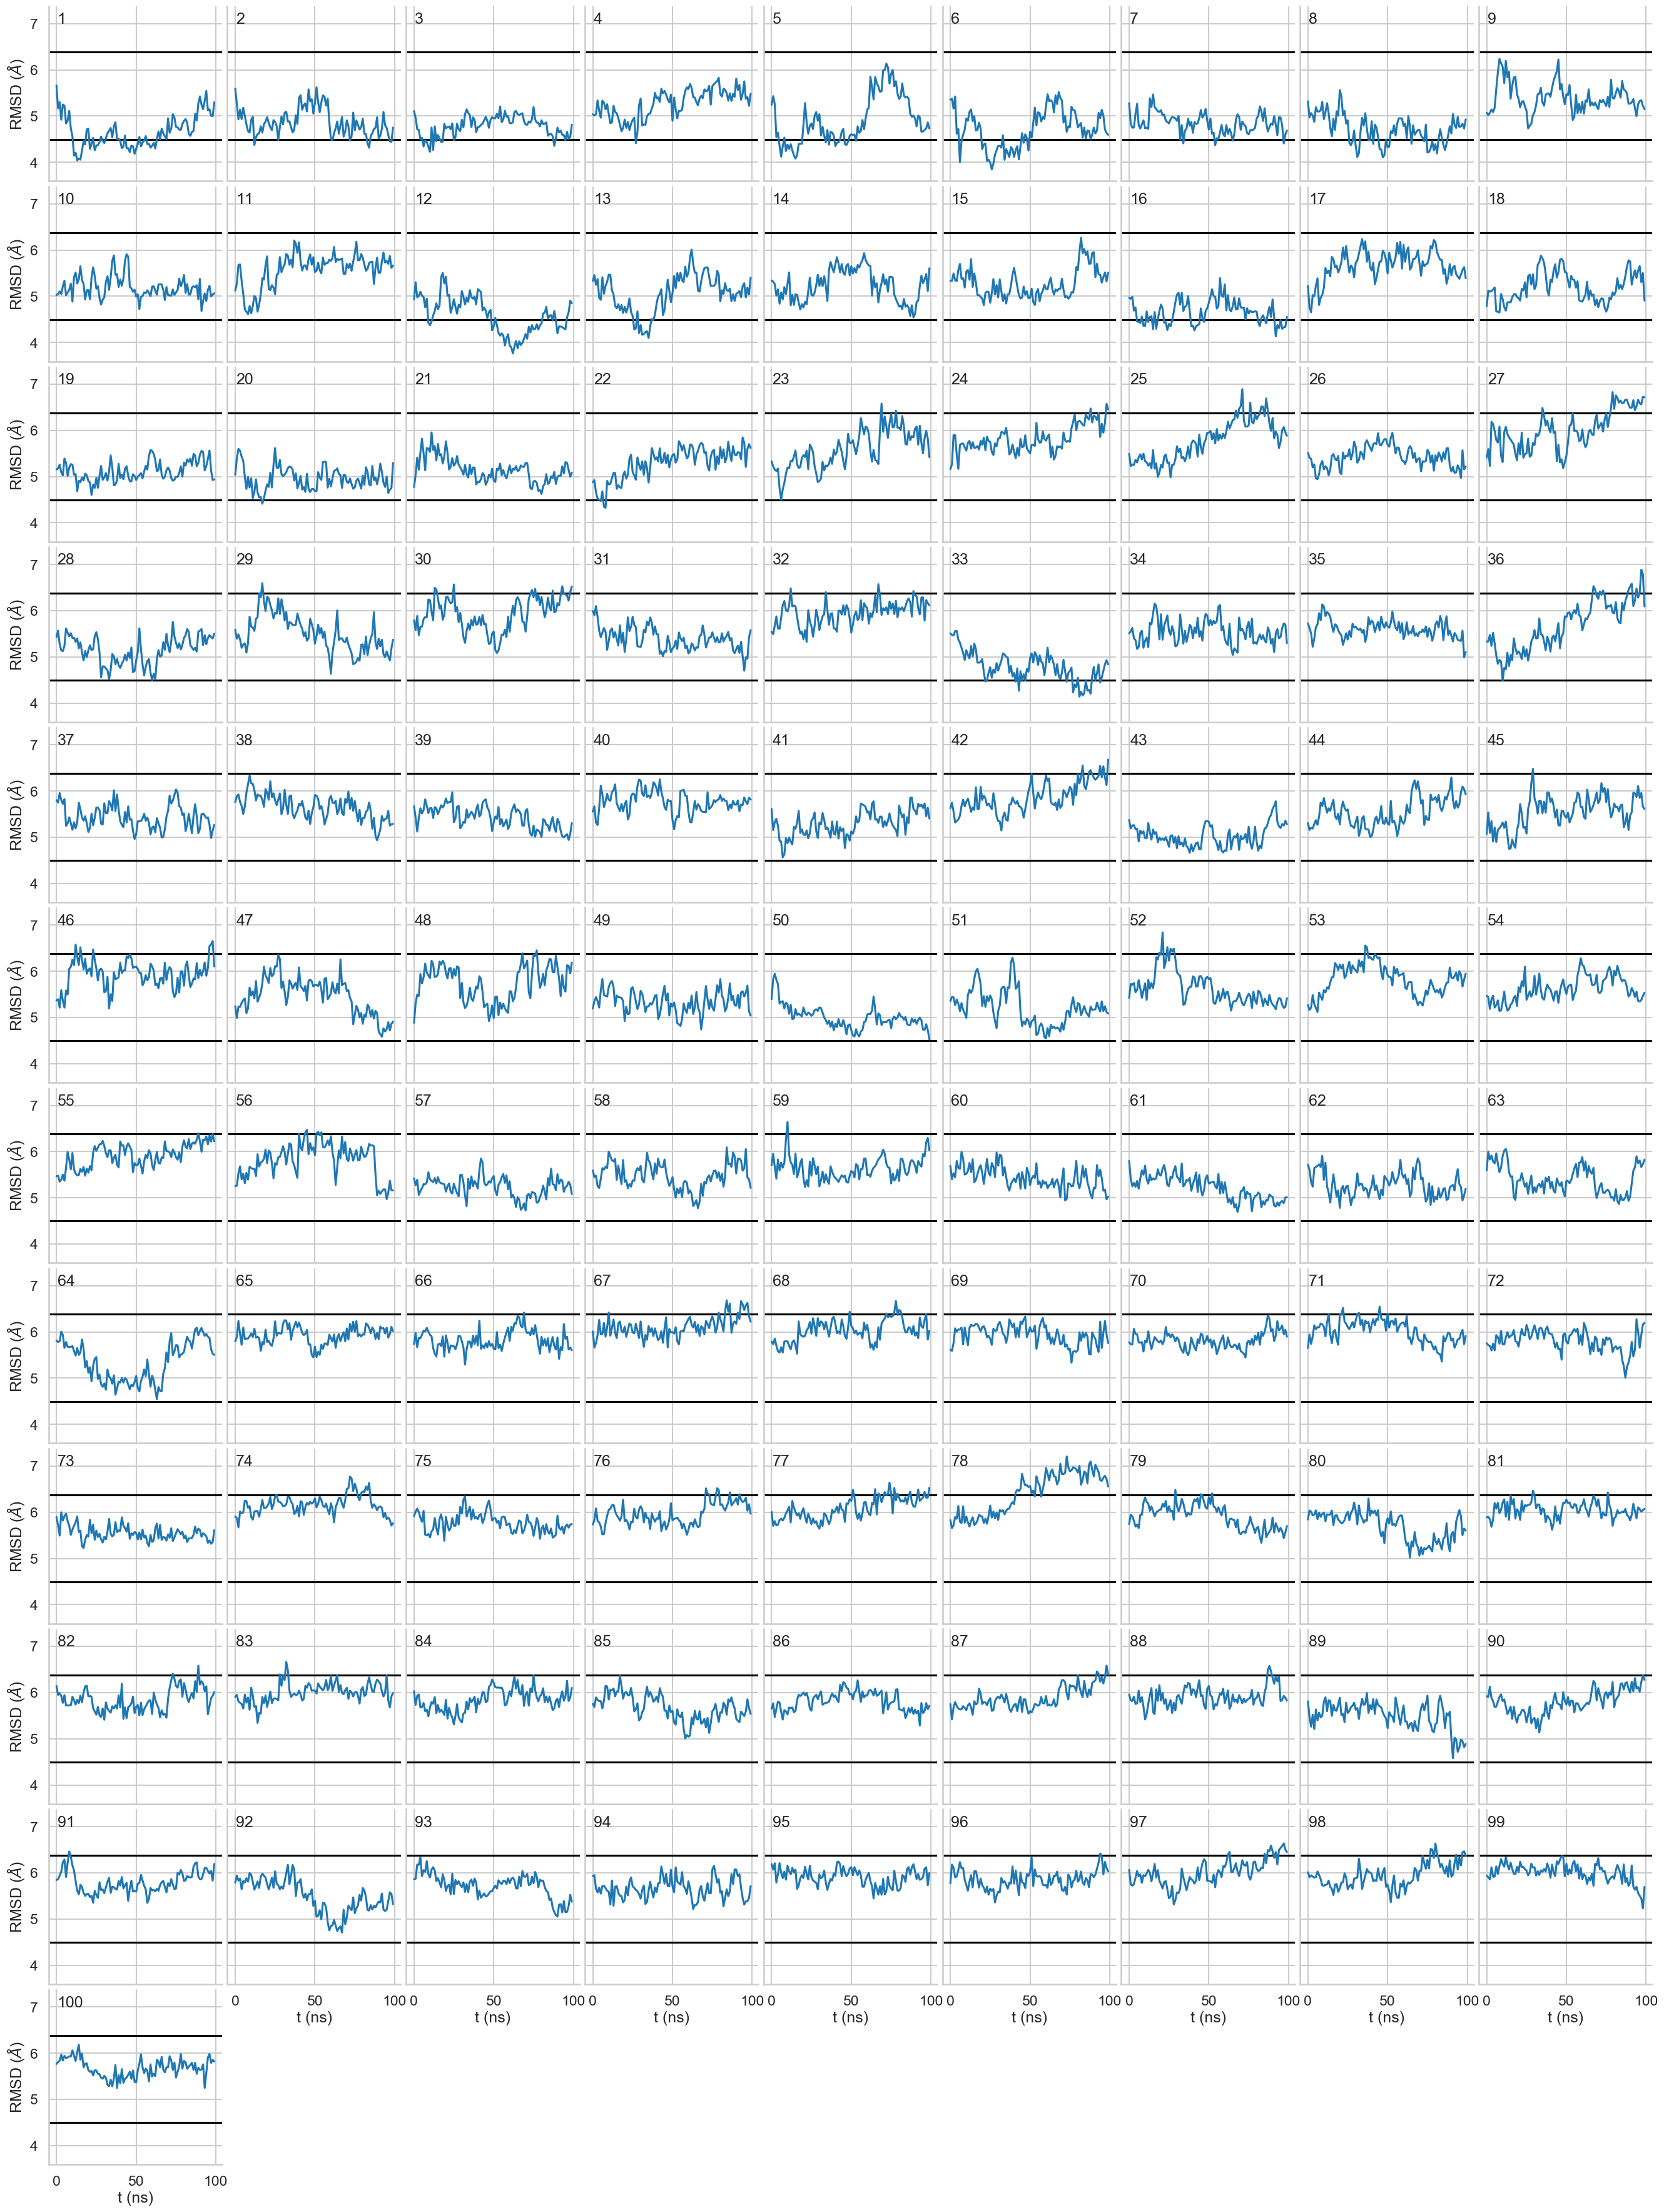
\includegraphics[width=0.9\textwidth]{chapters/aadh/figures/rmsd_backbone_ca.png}
 \label{fig:rmsd_ca}
\end{figure}

\begin{figure}[ph!]
 \centering
 \caption[Secondary structure composition of select trajectories]{\textsc{Secondary structure composition of trajectories $24, 27, 30, 42, 78, 87$ and $97$ as a function of time}. The number of residues in each simplified secondary structure class\cite{kabschDictionaryProteinSecondary1983} are shown: `H' (green) refers to alpha helix, 3- and 5-helices; `E' (orange) refers to residues in beta-bridges or beta ladder; `C' (blue) refers to turns, bends and all irregular elements.}
 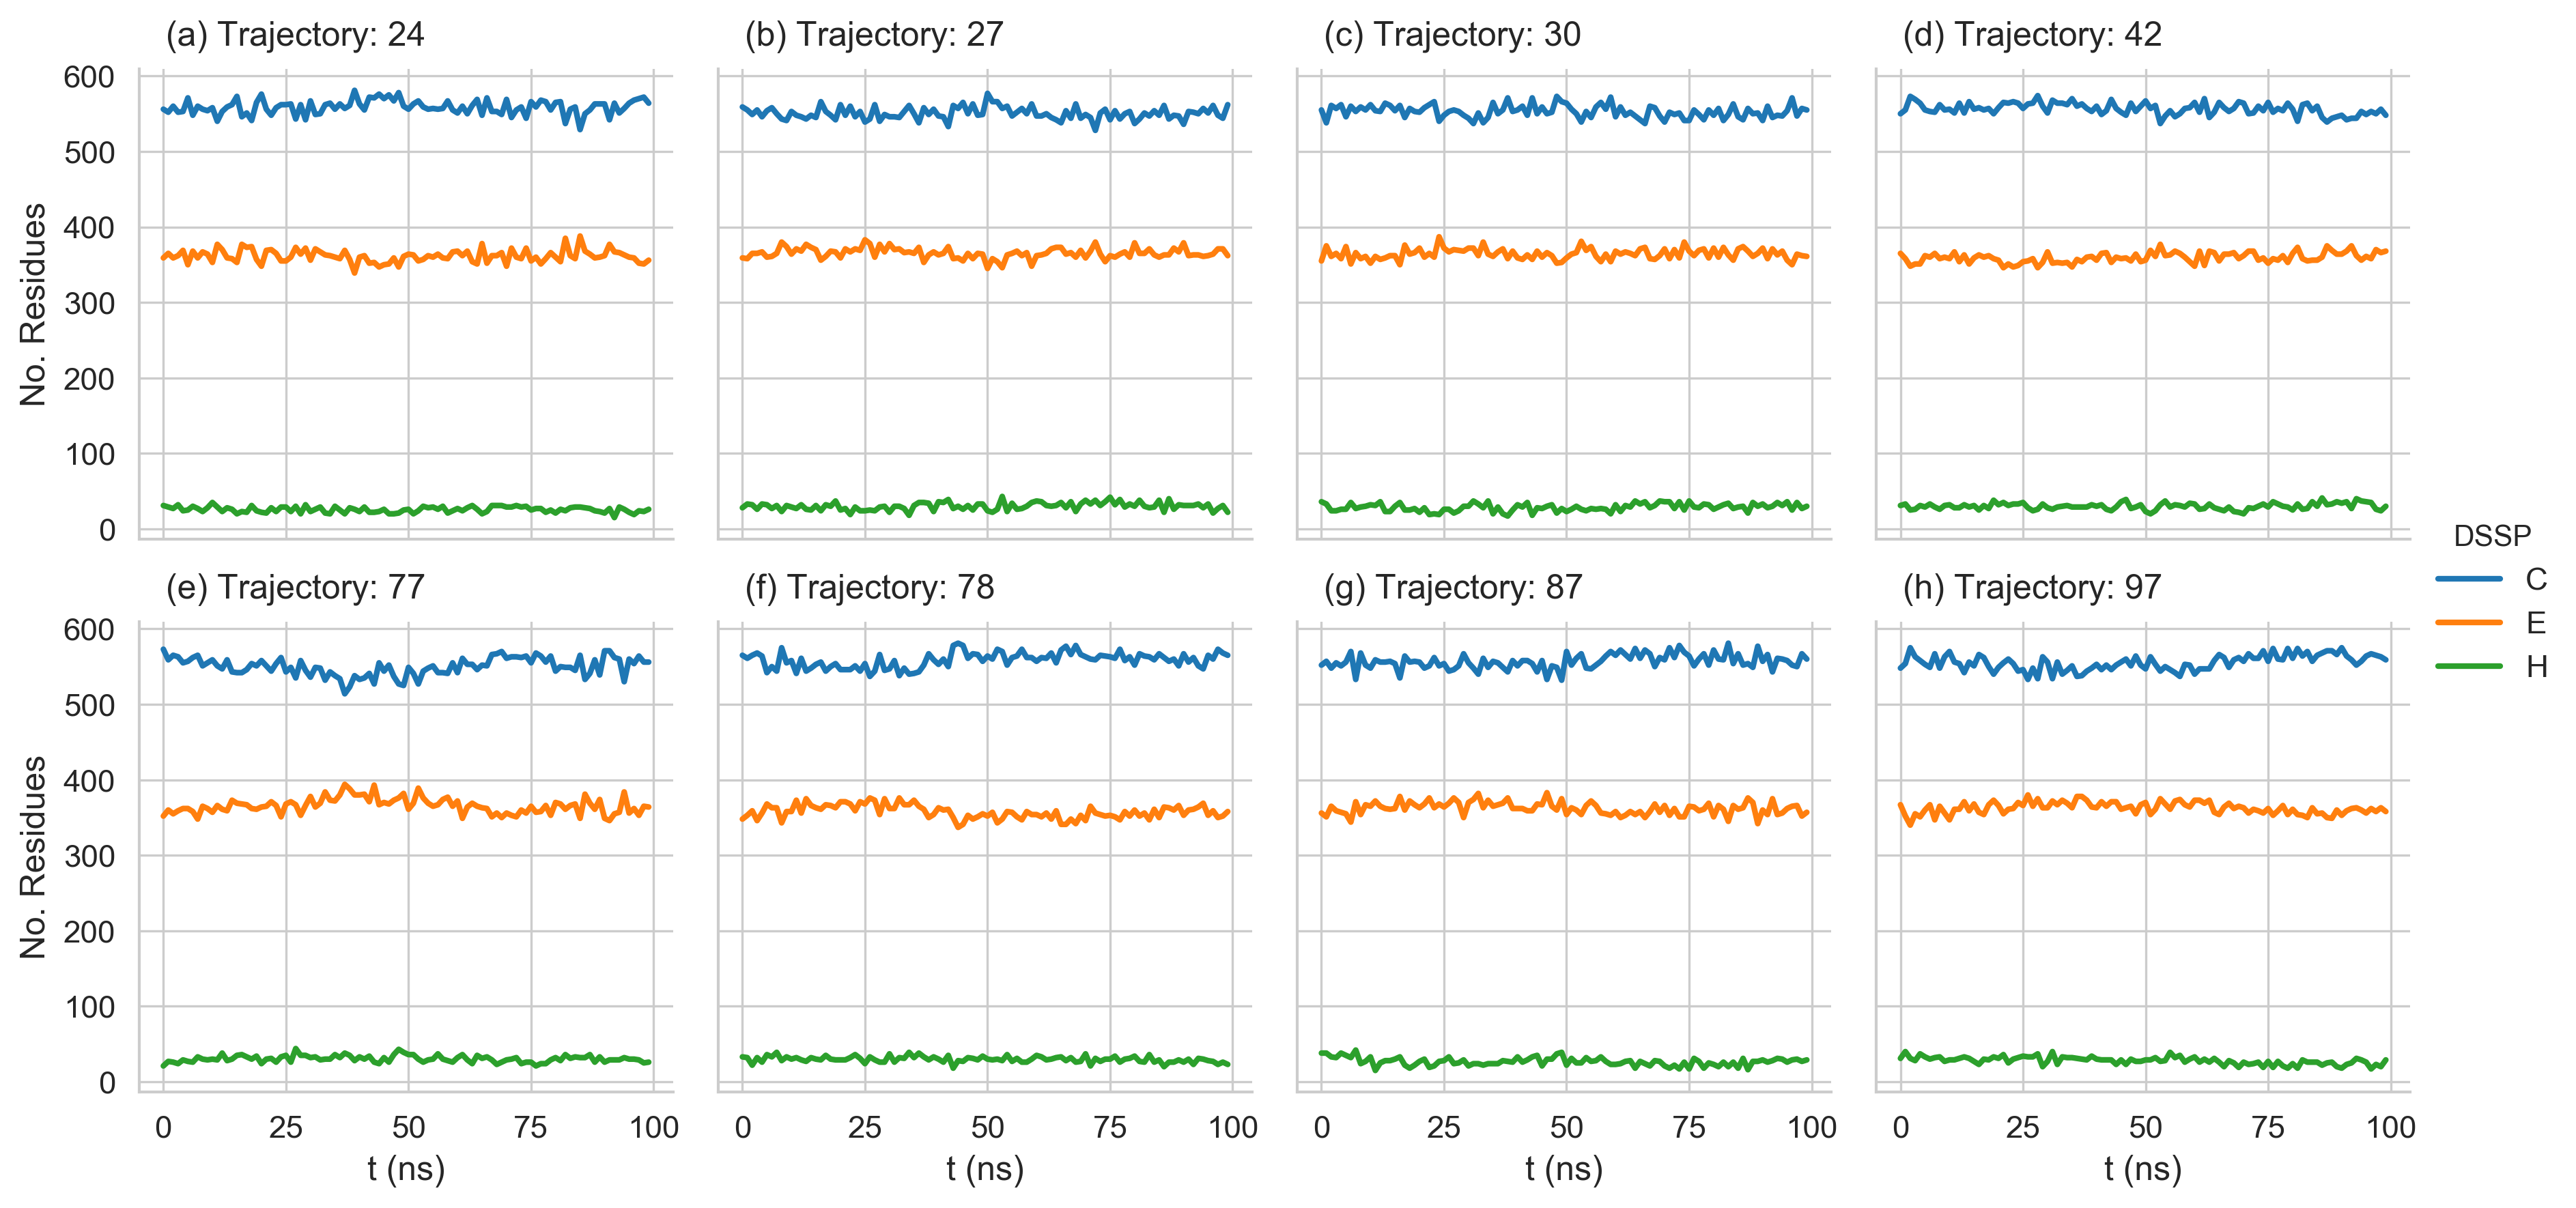
\includegraphics[width=0.9\textwidth]{chapters/aadh/figures/drift_trajs_dssp.png}
 \label{fig:dssp_trajs_sens}
\end{figure}

\begin{figure}[ph!]
    \centering
    \caption[Fluctuations in the deviation of residues of select trajectories]{\textsc{Fluctuations in the deviation of residues of trajectories $24, 27, 30, 42, 78, 87$ and $97$}. Each row corresponds to a different trajectory, each column to a different chain. \num{100} regularly spaced snapshots were taken from each trajectory and aligned to the crystal structure along with $\alpha$-carbon atoms. The standard deviation of the deviation of the $\alpha$-carbon atoms from the crystal structure, $\Delta\mathbf{r} = \mathbf{r}-\mathbf{r}_{\mathrm{crystal}}$ is plotted for each residue.}
    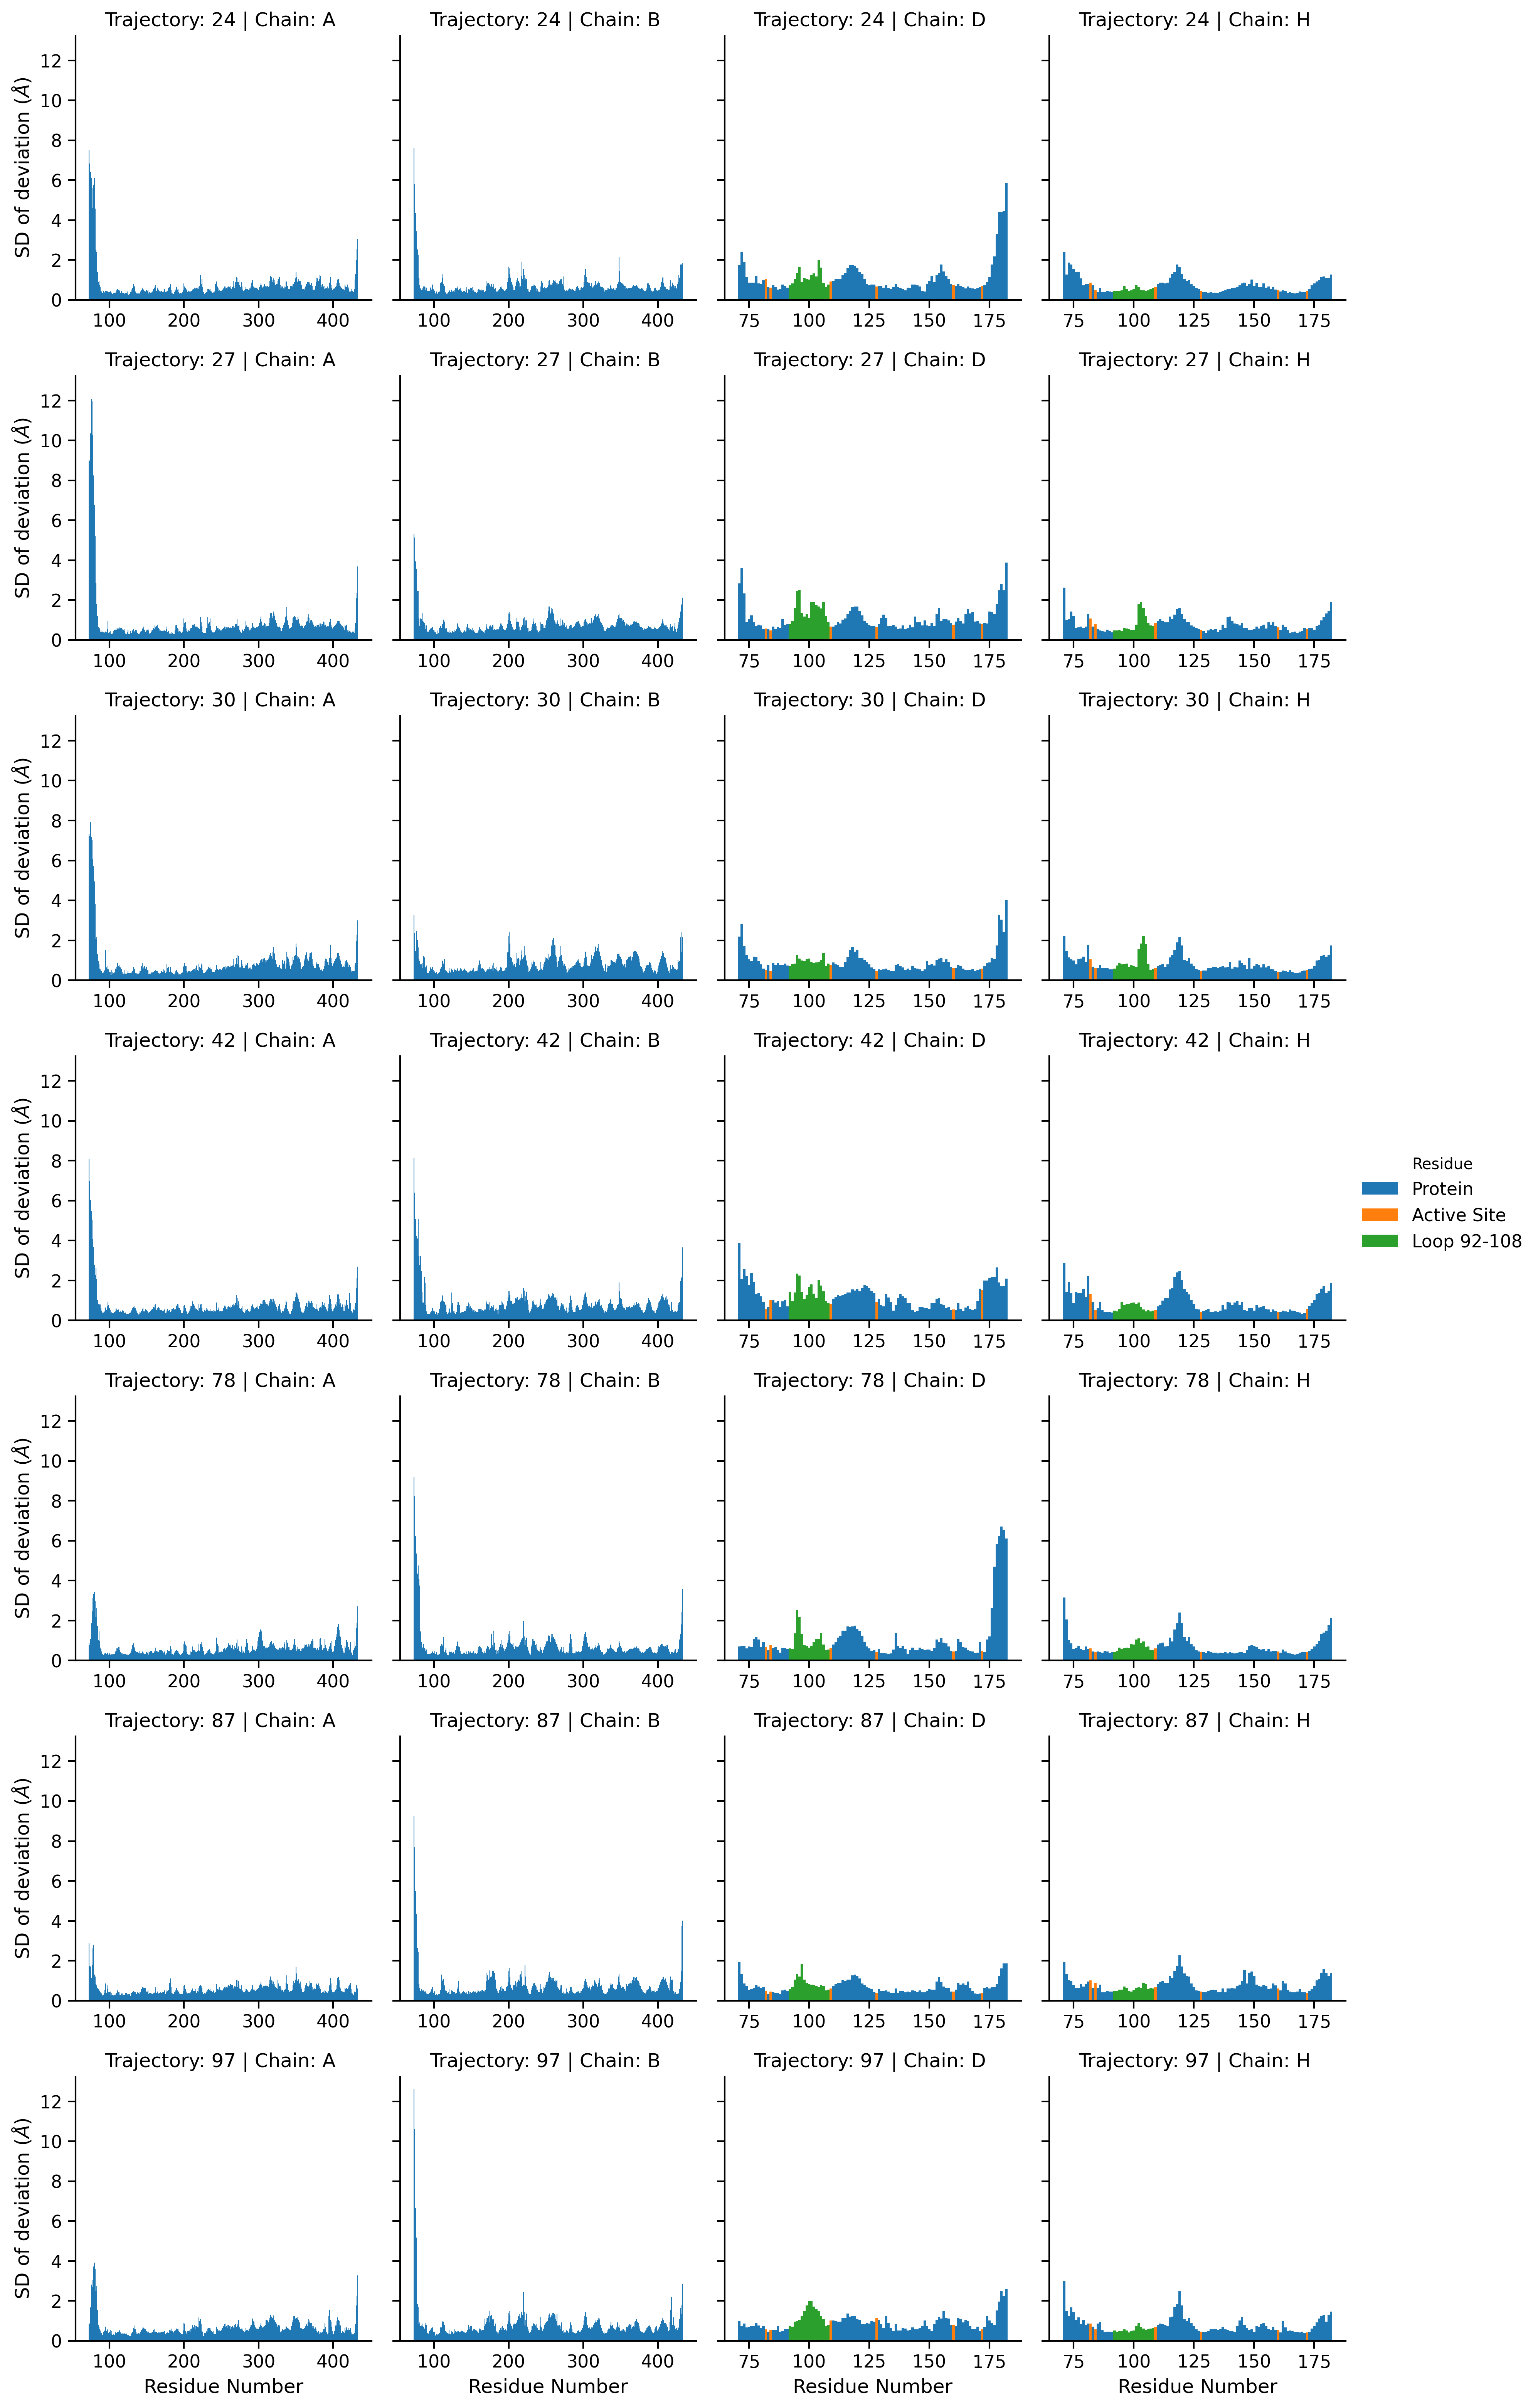
\includegraphics[height=0.8\textheight]{chapters/aadh/figures/sd_dev_by_residue.png}
    \label{fig:aadh_sd_dev_by_res}
\end{figure}

\begin{figure}[ph!]
 \centering
 \caption[Conformational change in loop residues 92-108 of chain D]{\textsc{Conformational change in loop residues \numrange[range-phrase=--]{92}{108} of chain D}. The crystal structure (left) and the seed trajectory at \SI{95}{\nano\second} (right) are shown from two different camera orientations (view 1 and view 2). The diameter of the backbone is proportional to the deviation of the $\alpha$-carbon from the crystal structure. The chart inset shows the deviation by residue of chain D, taken from figure \ref{fig:aadh_rmsd_byres}. The loop residues \numrange{92}{108} are highlighted in green, two active site residues TTW109 and Asp128 are shown in orange (the colour coding is consistent between the inset and the depicted conformations, except that four of the active site residues are not shown). The N-terminus (Glu71) and C-terminus (Lys181) are labelled. The \num{22} tail residues, unresolved by the crystal structure, are missing from the N-terminus.}
 \label{fig:chain_d_loop}
 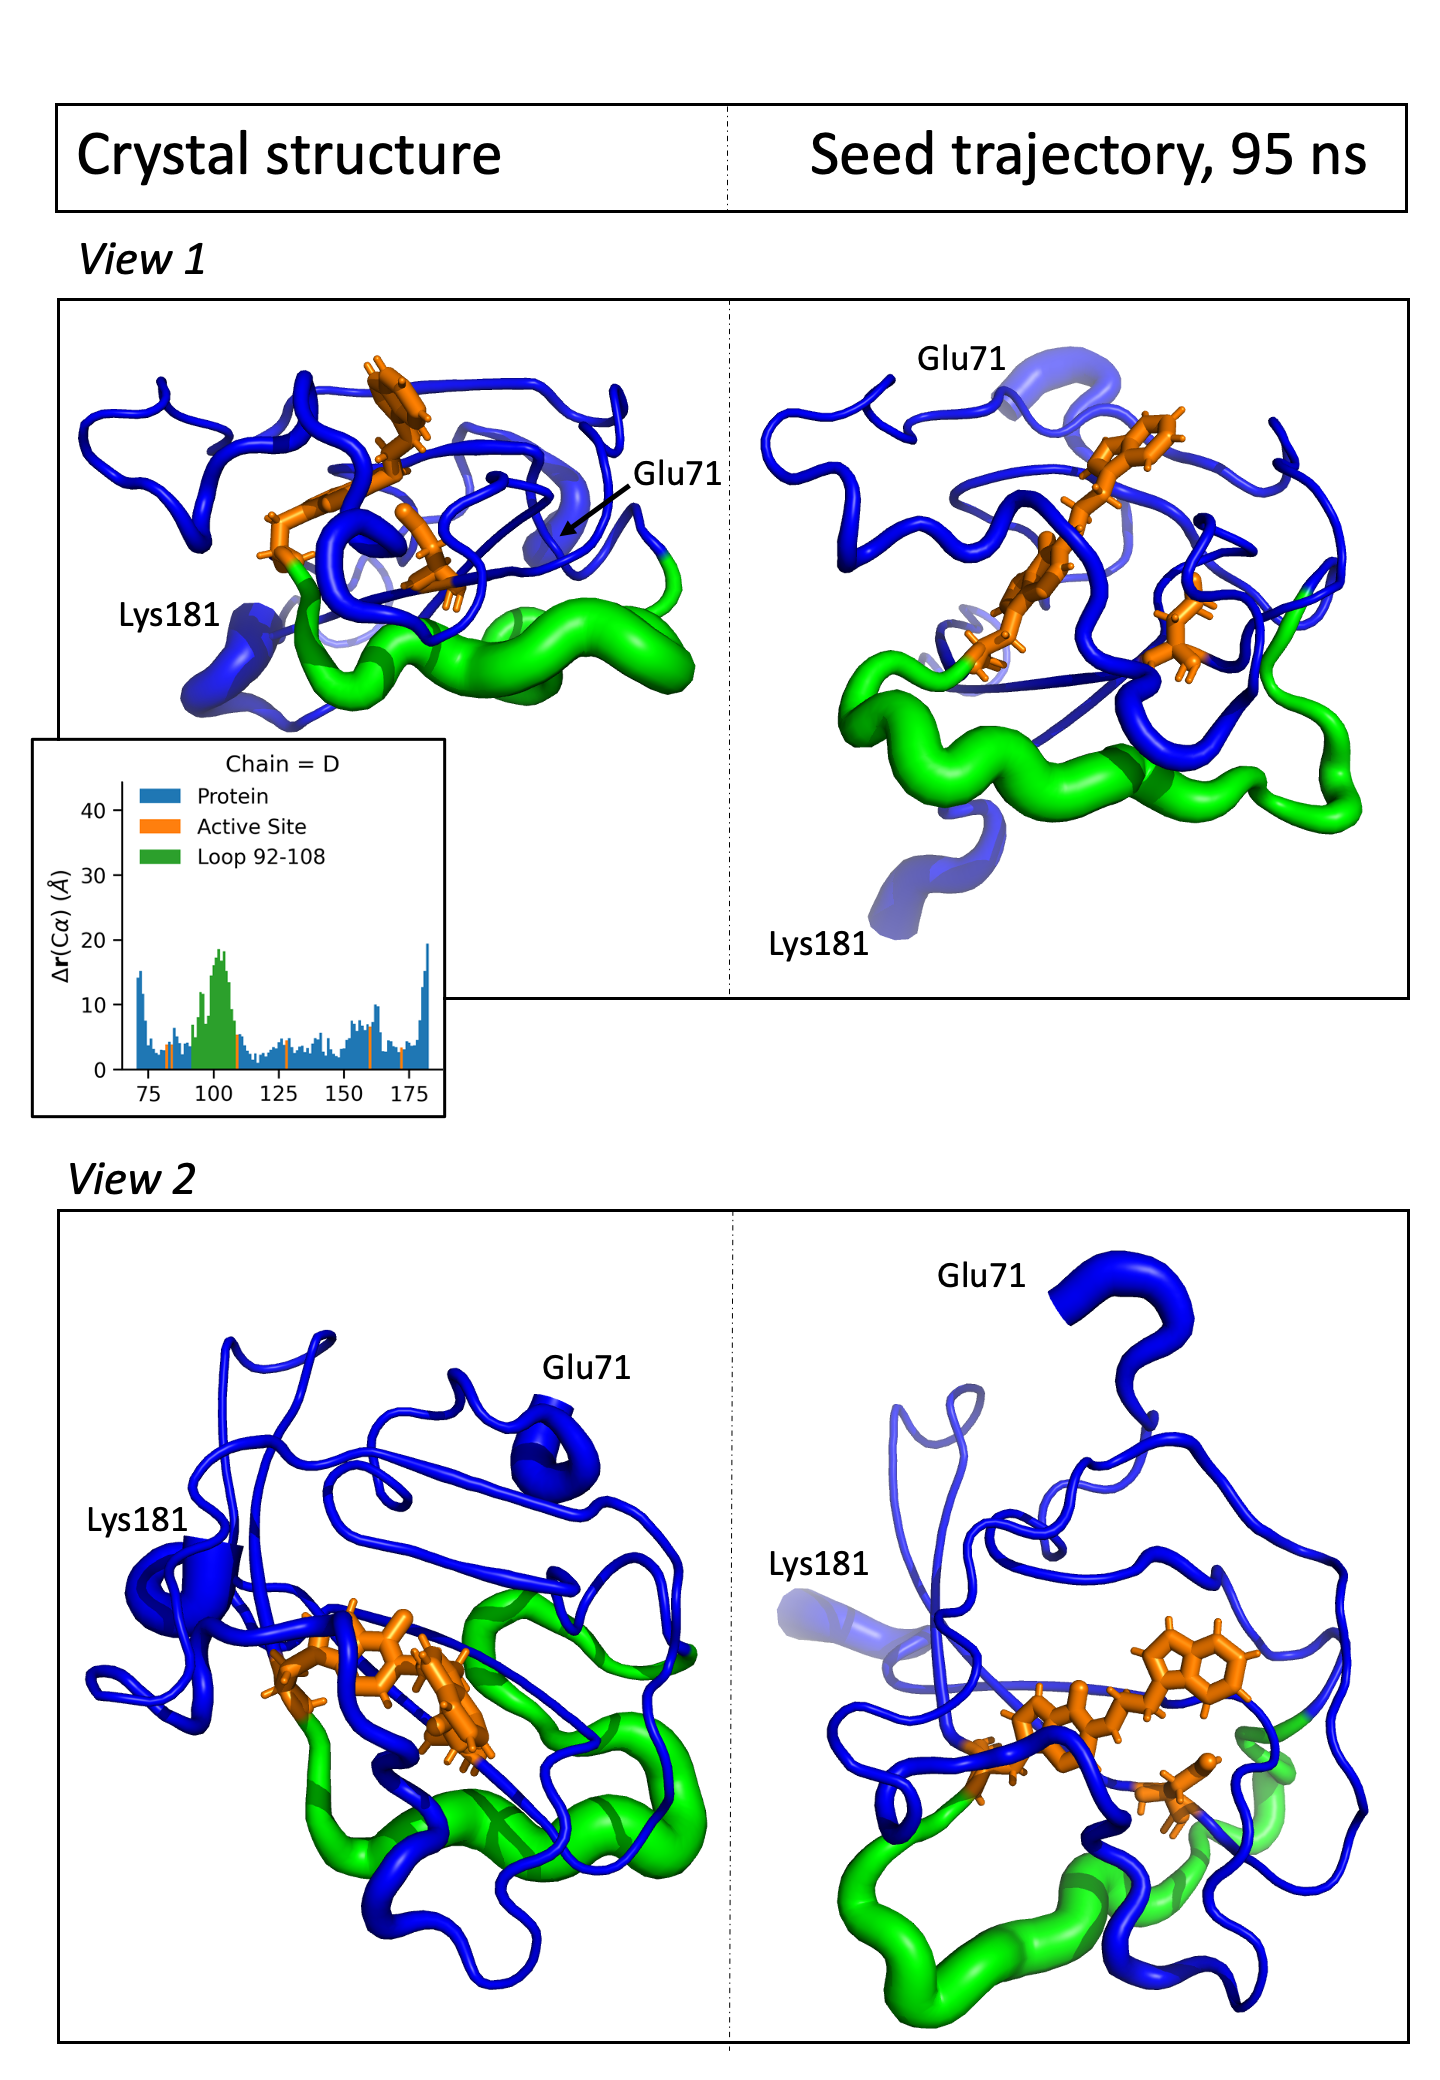
\includegraphics[height=0.75\textheight]{chapters/aadh/figures/rmsd_seg_d.png}
\end{figure}

% \section{MSM optimisation}

% \subsection{Estimating the Markov lag-time and number of metastable states}

\begin{figure}[ht!]
 \centering
 \caption[The ratio of successive eigenvalues and implied timescales of the sensitivity reference MSM]{\textsc{The ratio of successive eigenvalues and implied timescales of the sensitivity reference MSM}. Panel (a) shows the ratio of successive eigenvalues and panel (b) the implied timescales the sensitivity case of the reference MSM with: $\tau(\textrm{MSM})=\SI{2}{\nano\second}$, TICA lag time of $\tau=\SI{10}{\nano\second}$, \SI{95}{\percent} of the kinetic variance/$m=8$ TICA components retained, and $n=316$ microstates. Parameters were estimated using MCMC with \num{1000} posterior samples, the blue dots and error bars are the mean and \SI{95}{\percent} credible intervals respectively.}
 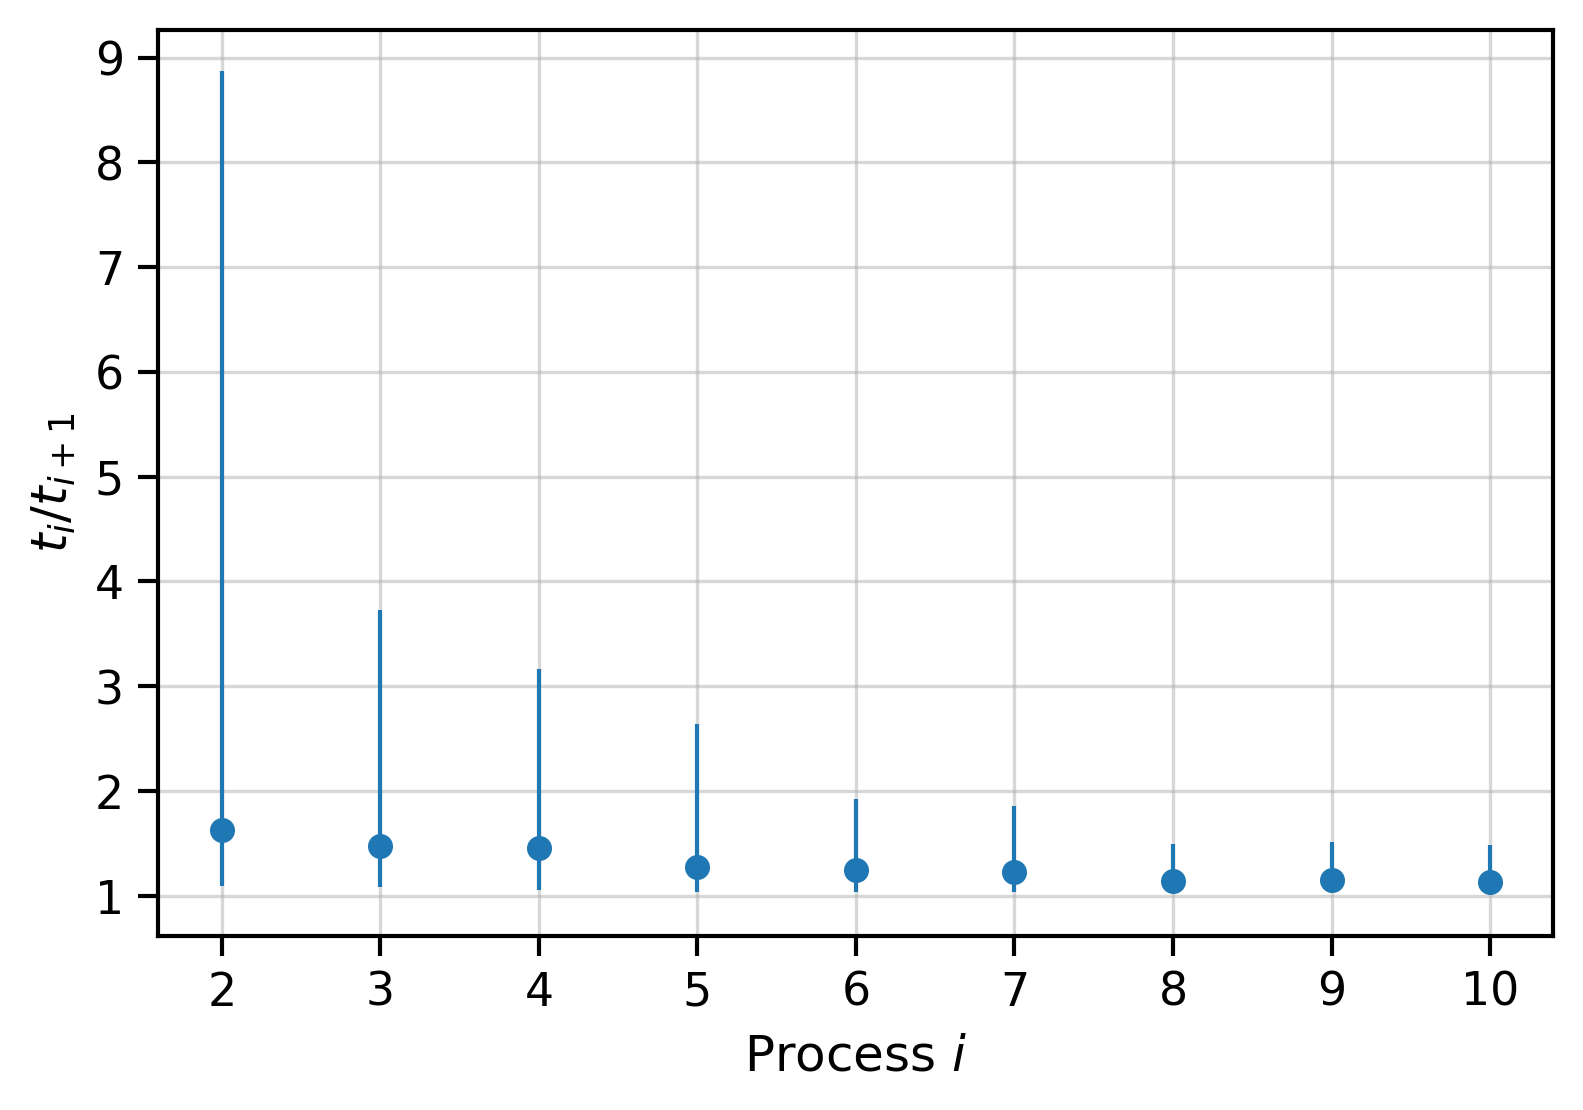
\includegraphics[width=0.8\textwidth]{chapters/aadh/figures/timescale_ratios_D_sens.png}
 \label{fig:ts_ratios_d_sens}
\end{figure}

\begin{figure}[ht!]
 \centering
    \caption[The implied timescales and VAMP-2 scores of the sensitivity reference MSM]{\textsc{The implied timescales and VAMP-2 scores of the reference MSM}. Panels (a) and (b) show the implied timescales, and panels (c) and (d) shows the relative VAMP-2 scores for the reference MSM with: $\tau(\textrm{MSM})=\SI{2}{\nano\second}$, TICA lag time of $\tau=\SI{10}{\nano\second}$, \SI{95}{\percent} of the kinetic variance/$m=10$ TICA components retained, and $n=316$ microstates. Panel (a) shows the first five implied timescales for $\tau(\mathrm{MSM})=\SIrange[range-phrase=--]{0.1}{5}{\nano\second}$, panel (b) shows the first five implied timescales for $\tau(\mathrm{MSM}) = \SIrange[range-phrase]{0.1}{50}{\nano\second}$. The solid lines and coloured shaded areas are the mean and \SI{95}{\percent} credible intervals respectively, estimated using MCMC with \num{500} posterior samples. The grey shaded area is the region for which the implied timescales are smaller than the lag time. Panel (c) and (d) show the VAMP-2 scores, scored on the first \numrange{2}{5} eigenvalues for the same ranges. The VAMP-2 scores are indexed to their value at $\tau(\mathrm{MSM})=\SI{0.1}{\nano\second}$. The colour coding is consistent between the implied timescale plots ((a) and (b)) and VAMP-2 plots ((c) and (d)). e.g. the blue line in (c) and (d) is the VAMP-2 score with two eigenvalues ($r=2$) while in (a) and (b) blue is the second implied timescale, $t_{2}$.}
 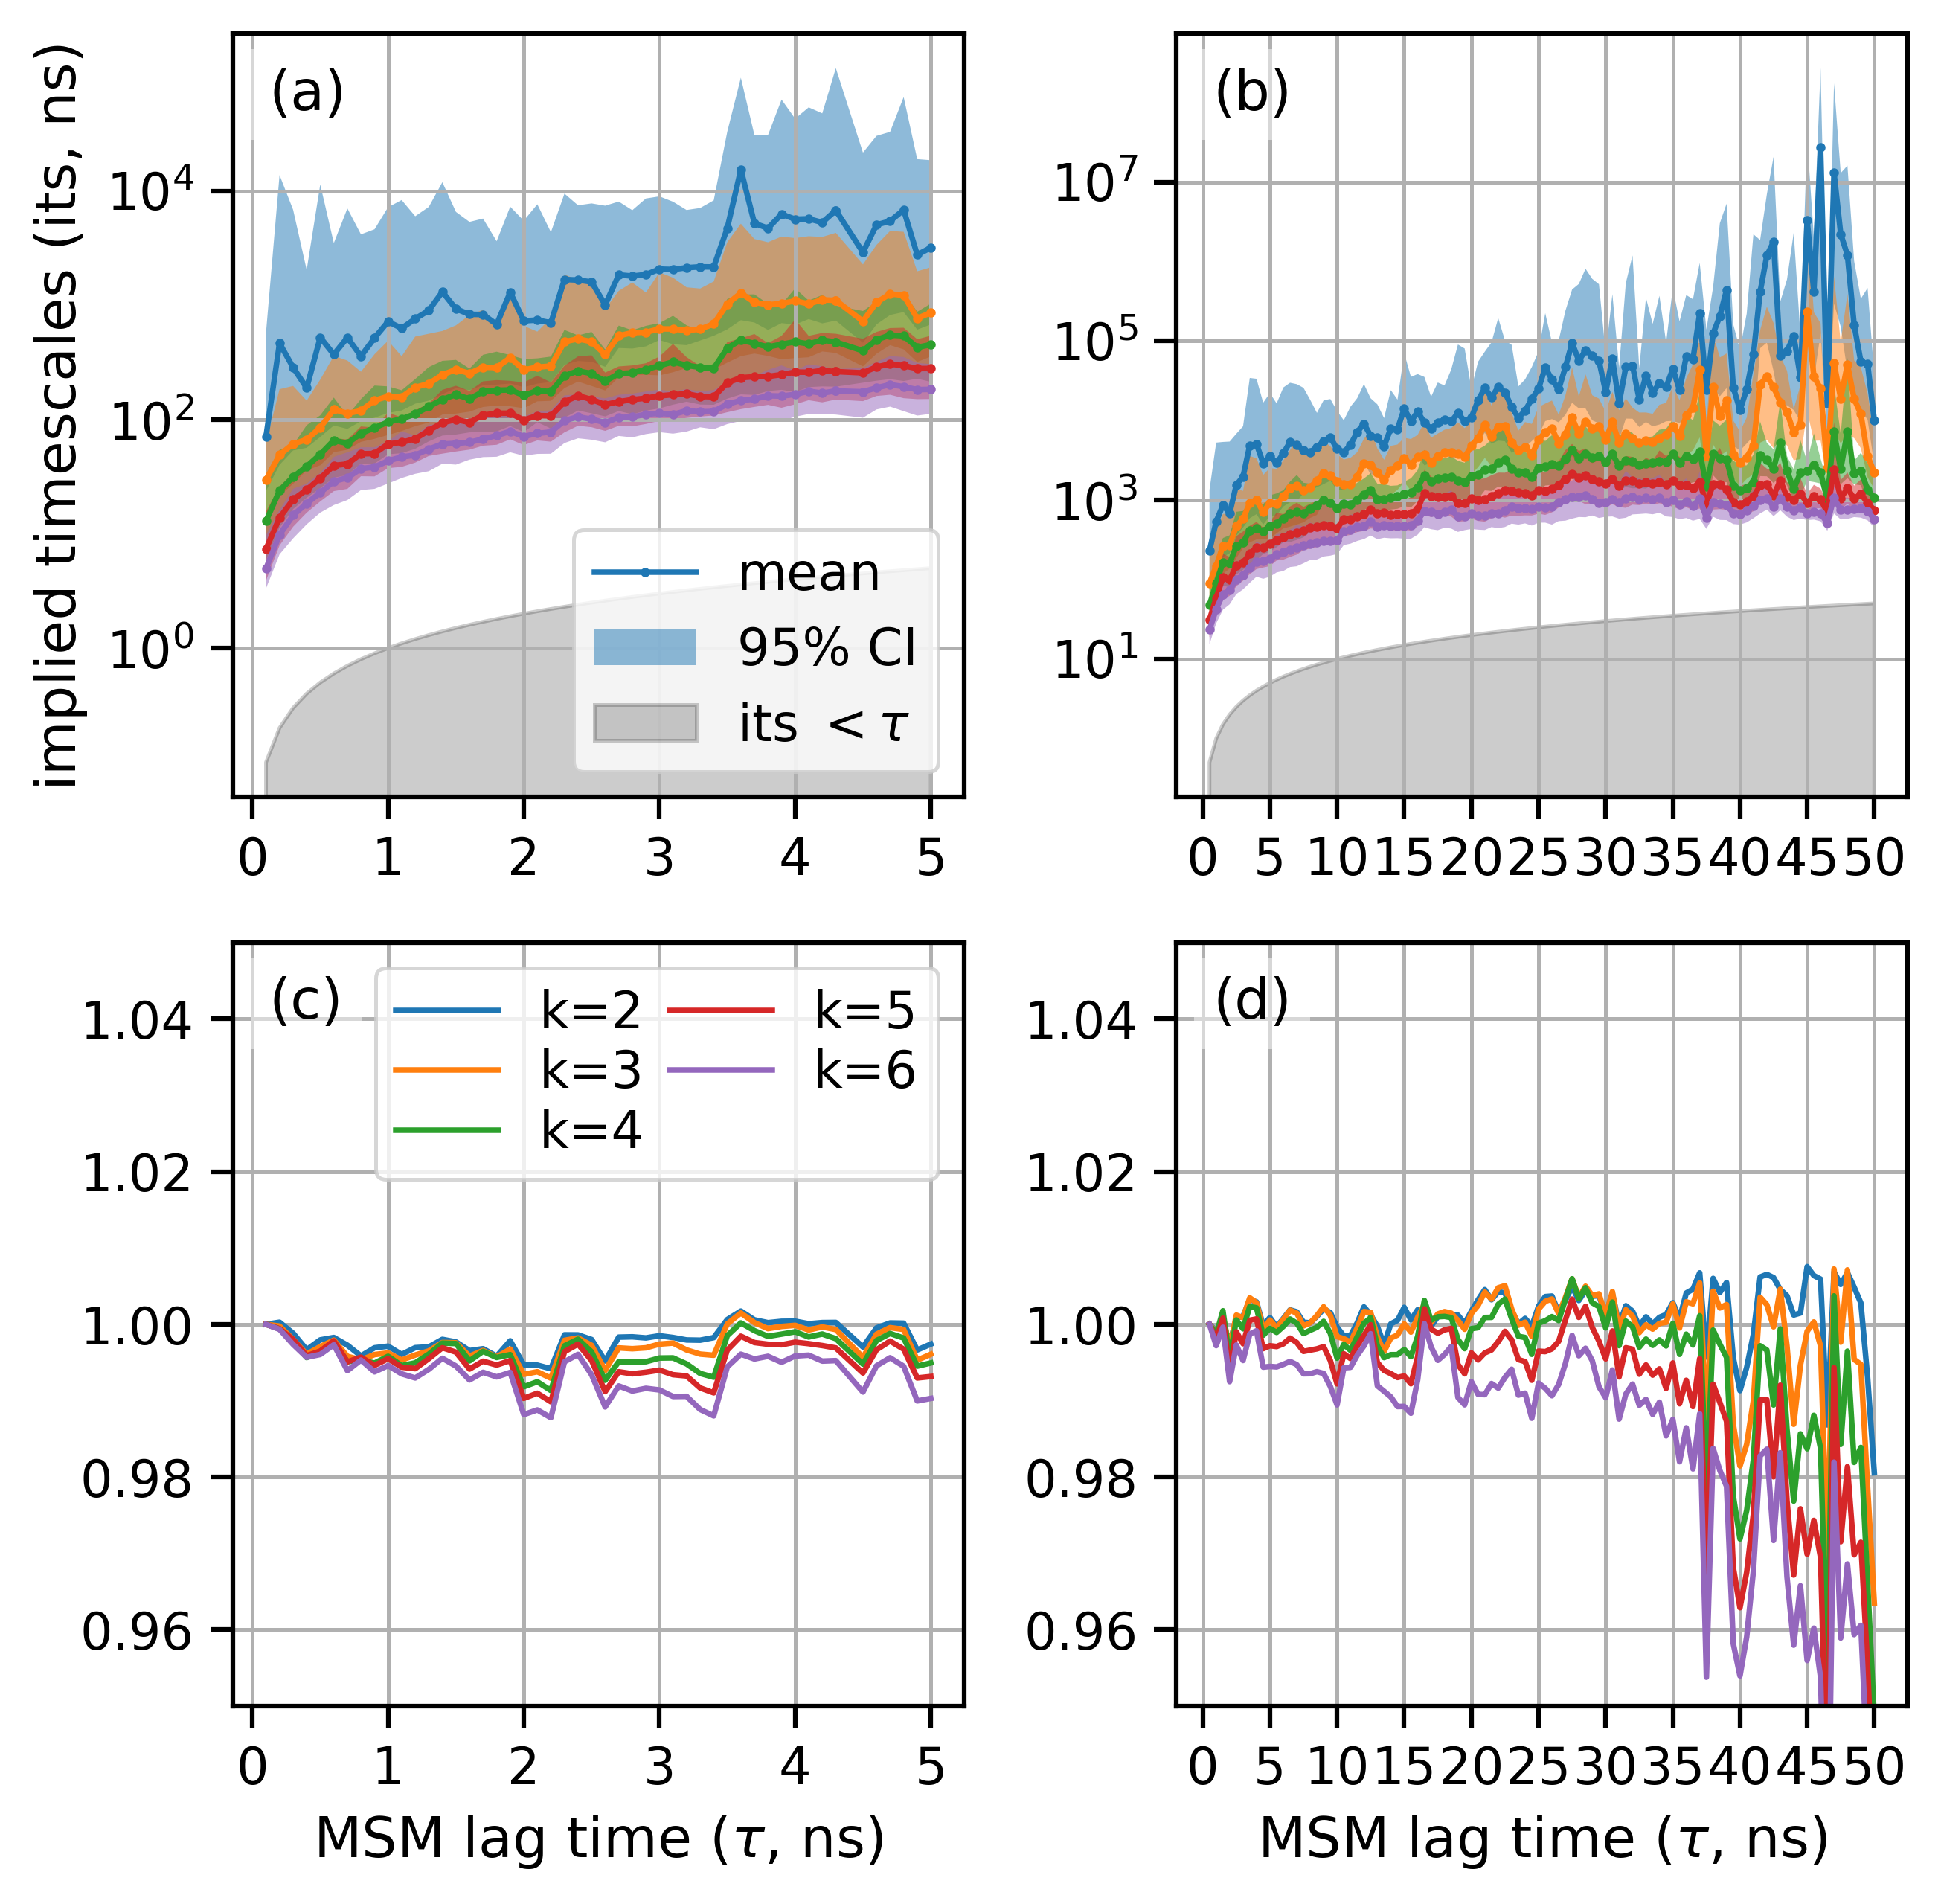
\includegraphics[width=0.8\textwidth]{chapters/aadh/figures/implied_timescales_D_sens.png}
 \label{fig:its_d_sens}
\end{figure}

% \subsection{Response surface}\label{app:msm_rsm}

% \subsubsection{GP model selection metrics}
\begin{table}[ht!]
 \centering
 \caption[Gaussian process model selection metrics for the response surface of AADH using all randomly sampled hyperparameter trials]{\textsc{Gaussian process model selection metrics for the response surface of AADH using all randomly sampled hyperparameter trials, $\mathcal{D}_{361}$}. The mean standardised log loss (MSLL) and standardised mean square error (SMSE) where calculated using 10 fold cross validation. Only those models which had both $\mathrm{MSLL}<0$ and $\mathrm{SMSE}<1$ were ranked. The total rank is calculated as rank of $\sqrt{R_{\mathrm{MSLL}}^{2}+R_{\mathrm{SMSE}}^2}$. Where the overall rank was tied, the first model appearing in the table was ranked higher.}
 \label{tab:aadh_rsm_metrics_all_data}
 \begin{tabularx}{1\textwidth}{llllrr >{\raggedleft\arraybackslash}X>{\raggedleft\arraybackslash}X>{\raggedleft\arraybackslash}X}
 \toprule
 $T(\tau)$ & $T(m)$ & $T(n)$ & Kernel & MSLL & SMSE & Rank (MSLL) & Rank (SMSE) & Rank (Total)\\
 \midrule
 $I({\tau})$ & $I({m})$ & $I({n})$ & Exponential & -0.1298 & 0.3087 & 1.0 & 1.0 & 1.0 \\
   &  & $\log({n})$ & Exponential & 0.0050 & 0.2964 &  - &  - & - \\
   & $\log({m})$ & $I({n})$ & Exponential & 0.0521 & 0.3118 &  - &  - & - \\
   &  & $\log({n})$ & Exponential & 0.5633 & 0.3815 &  - &  - & - \\
 $\log({\tau})$ & $I({m})$ & $I({n})$ & Exponential & 0.1967 & 0.3436 &  - &  - & - \\
   &  & $\log({n})$ & Exponential & 0.4959 & 0.3231 &  - &  - & - \\
   & $\log({m})$ & $I({n})$ & Exponential & 0.5128 & 0.4365 &  - &  - & - \\
   &  & $\log({n})$ & Exponential & 1.0267 & 0.4201 &  - &  - & - \\
 $I({\tau})$ & $I({m})$ & $I({n})$ & Mat{\'e}rn 3-2 & 1.5680 & 0.2893 &  - &  - & - \\
   &  & $\log({n})$ & Mat{\'e}rn 3-2 & 1.9193 & 0.2960 &  - &  - & - \\
   & $\log({m})$ & $I({n})$ & Mat{\'e}rn 3-2 & 3.1385 & 0.2775 &  - &  - & - \\
   &  & $\log({n})$ & Mat{\'e}rn 3-2 & 2.0358 & 0.2818 &  - &  - & - \\
 $\log({\tau})$ & $I({m})$ & $I({n})$ & Mat{\'e}rn 3-2 & 6.9015 & 0.3203 &  - &  - & - \\
   &  & $\log({n})$ & Mat{\'e}rn 3-2 & 7.7182 & 0.3406 &  - &  - & - \\
   & $\log({m})$ & $I({n})$ & Mat{\'e}rn 3-2 & 7.9209 & 0.3257 &  - &  - & - \\
   &  & $\log({n})$ & Mat{\'e}rn 3-2 & 3.0002 & 0.3472 &  - &  - & - \\
 $I({\tau})$ & $I({m})$ & $I({n})$ & Mat{\'e}rn 5-2 & 3.6517 & 0.3029 &  - &  - & - \\
   &  & $\log({n})$ & Mat{\'e}rn 5-2 & 3.8316 & 0.3090 &  - &  - & - \\
   & $\log({m})$ & $I({n})$ & Mat{\'e}rn 5-2 & 8.6574 & 0.2991 &  - &  - & - \\
   &  & $\log({n})$ & Mat{\'e}rn 5-2 & 3.7354 & 0.3238 &  - &  - & - \\
 $\log({\tau})$ & $I({m})$ & $I({n})$ & Mat{\'e}rn 5-2 & 8.9207 & 0.3679 &  - &  - & - \\
   &  & $\log({n})$ & Mat{\'e}rn 5-2 & 11.8753 & 0.4064 &  - &  - & - \\
   & $\log({m})$ & $I({n})$ & Mat{\'e}rn 5-2 & 12.7637 & 0.3722 &  - &  - & - \\
   &  & $\log({n})$ & Mat{\'e}rn 5-2 & 13.6735 & 0.3475 &  - &  - & - \\
 $I({\tau})$ & $I({m})$ & $I({n})$ & Gaussian & inf & inf &  - &  - & - \\
   &  & $\log({n})$ & Gaussian & 9.3618 & 0.3256 &  - &  - & - \\
   & $\log({m})$ & $I({n})$ & Gaussian & 5.9123 & 0.3022 &  - &  - & - \\
   &  & $\log({n})$ & Gaussian & inf & inf &  - &  - & - \\
 $\log({\tau})$ & $I({m})$ & $I({n})$ & Gaussian & 17.4786 & 0.4551 &  - &  - & - \\
   &  & $\log({n})$ & Gaussian & 16.7568 & 0.3556 &  - &  - & - \\
   & $\log({m})$ & $I({n})$ & Gaussian & 16.7412 & 0.5026 &  - &  - & - \\
   &  & $\log({n})$ & Gaussian & 24.3199 & 0.4986 &  - &  - & - \\
 \bottomrule
 \end{tabularx}
\end{table}



\begin{table}[ht!]
 \centering
 \caption[Gaussian process model selection metrics for the response surface of AADH using hyperparameter trial data subset 1]{\textsc{Gaussian process model selection metrics for the response surface of AADH using hyperparameter trial data subset 1, $\mathcal{D}^{1}_{100}$}. The mean standardised log loss (MSLL) and standardised mean square error (SMSE) where calculated using 10 fold cross validation. Only those models which had both $\mathrm{MSLL}<0$ and $\mathrm{SMSE}<1$ were ranked. The total rank is calculated as rank of $\sqrt{R_{\mathrm{MSLL}}^{2}+R_{\mathrm{SMSE}}^2}$. Where the overall rank was tied, the first model appearing in the table was ranked higher.}
 \label{tab:aadh_rsm_metrics_iter_1}
 \begin{tabularx}{1\textwidth}{llllrr >{\raggedleft\arraybackslash}X>{\raggedleft\arraybackslash}X>{\raggedleft\arraybackslash}X}
 \toprule
 $T(\tau)$ & $T(m)$ & $T(n)$ & Kernel & MSLL & SMSE & Rank (MSLL) & Rank (SMSE) & Rank (Total)\\
 \midrule
 $I({\tau})$ & $I({m})$ & $I({n})$ & Exponential & -0.3928 & 0.3412 & 10.0 & 14.0 &  13.0 \\
  &  & $\log({n})$ & Exponential & -0.2456 & 0.3443 & 15.0 & 15.0 &  16.0 \\
  & $\log({m})$ & $I({n})$ & Exponential & -0.6484 & 0.3169 &  6.0 & 12.0 &  7.0 \\
  &  & $\log({n})$ & Exponential & -0.5585 & 0.3487 &  7.0 & 17.0 &  14.0 \\
 $\log({\tau})$ & $I({m})$ & $I({n})$ & Exponential & 0.0598 & 0.3483 &  - &  - &  - \\
   &  & $\log({n})$ & Exponential & -0.2195 & 0.3450 & 16.0 & 16.0 &  17.0 \\
   & $\log({m})$ & $I({n})$ & Exponential & -0.3524 & 0.3084 & 13.0 &  9.0 &  10.0 \\
   &  & $\log({n})$ & Exponential & -0.3944 & 0.3379 &  9.0 & 13.0 &  11.0 \\
 $I({\tau})$ & $I({m})$ & $I({n})$ & Mat{\'e}rn 3-2 & -0.3807 & 0.3167 & 12.0 & 11.0 &  12.0 \\
   &  & $\log({n})$ & Mat{\'e}rn 3-2 & -0.2744 & 0.3053 & 14.0 &  7.0 &  9.0 \\
   & $\log({m})$ & $I({n})$ & Mat{\'e}rn 3-2 & -0.8769 & 0.2779 &  1.0 &  4.0 &  3.0 \\
   &  & $\log({n})$ & Mat{\'e}rn 3-2 & -0.7438 & 0.2785 &  5.0 &  5.0 &  5.0 \\
 $\log({\tau})$ & $I({m})$ & $I({n})$ & Mat{\'e}rn 3-2 & 0.3415 & 0.3721 &  - &  - &  - \\
   &  & $\log({n})$ & Mat{\'e}rn 3-2 & -0.2023 & 0.3892 & 17.0 & 18.0 &  18.0 \\
   & $\log({m})$ & $I({n})$ & Mat{\'e}rn 3-2 & -0.4758 & 0.3033 &  8.0 &  6.0 &  6.0 \\
   &  & $\log({n})$ & Mat{\'e}rn 3-2 & -0.3892 & 0.3086 & 11.0 & 10.0 &  8.0 \\
 $I({\tau})$ & $I({m})$ & $I({n})$ & Mat{\'e}rn 5-2 & 0.3362 & 0.3149 &  - &  - &  - \\
   &  & $\log({n})$ & Mat{\'e}rn 5-2 & 0.9964 & 0.2712 &  - &  - &  - \\
   & $\log({m})$ & $I({n})$ & Mat{\'e}rn 5-2 & -0.8713 & 0.2685 &  2.0 &  2.0 &  1.0 \\
   &  & $\log({n})$ & Mat{\'e}rn 5-2 & -0.7508 & 0.2700 &  4.0 &  3.0 &  4.0 \\
 $\log({\tau})$ & $I({m})$ & $I({n})$ & Mat{\'e}rn 5-2 & 6.4201 & 0.3503 &  - &  - &  - \\
   &  & $\log({n})$ & Mat{\'e}rn 5-2 & 5.7695 & 0.3250 &  - &  - &  - \\
   & $\log({m})$ & $I({n})$ & Mat{\'e}rn 5-2 & 3.9718 & 0.3153 &  - &  - &  - \\
   &  & $\log({n})$ & Mat{\'e}rn 5-2 & inf & inf &  - &  - &  - \\
 $I({\tau})$ & $I({m})$ & $I({n})$ & Gaussian & -0.1677 & 0.3074 & 18.0 &  8.0 &  15.0 \\
   &  & $\log({n})$ & Gaussian & 1.3068 & 0.2747 &  - &  - &  - \\
   & $\log({m})$ & $I({n})$ & Gaussian & -0.7884 & 0.2675 &  3.0 &  1.0 &  2.0 \\
   &  & $\log({n})$ & Gaussian & inf & inf &  - &  - &  - \\
 $\log({\tau})$ & $I({m})$ & $I({n})$ & Gaussian & 6.8541 & 0.3472 &  - &  - &  - \\
   &  & $\log({n})$ & Gaussian & 6.2984 & 0.3074 &  - &  - &  - \\
   & $\log({m})$ & $I({n})$ & Gaussian & 4.8742 & 0.4157 &  - &  - &  - \\
   &  & $\log({n})$ & Gaussian & 7.6739 & 0.5531 &  - &  - &  - \\
 \bottomrule
 \end{tabularx}
\end{table}

\begin{table}[ht!]
 \centering
 \caption[Gaussian process model selection metrics for the response surface of AADH using hyperparameter trial data subset 2]{\textsc{Gaussian process model selection metrics for the response surface of AADH using hyperparameter trial data subset 2, $\mathcal{D}^{2}_{100}$}. The mean standardised log loss (MSLL) and standardised mean square error (SMSE) where calculated using 10 fold cross validation. Only those models which had both $\mathrm{MSLL}<0$ and $\mathrm{SMSE}<1$ were ranked. The total rank is calculated as rank of $\sqrt{R_{\mathrm{MSLL}}^{2}+R_{\mathrm{SMSE}}^2}$. Where the overall rank was tied, the first model appearing in the table was ranked higher.}
 \label{tab:aadh_rsm_metrics_iter_2}
 \begin{tabularx}{1\textwidth}{llllrr >{\raggedleft\arraybackslash}X>{\raggedleft\arraybackslash}X>{\raggedleft\arraybackslash}X}
 \toprule
 $T(\tau)$ & $T(m)$ & $T(n)$ & Kernel & MSLL & SMSE & Rank (MSLL) & Rank (SMSE) & Rank (Total)\\
 \midrule
 $I({\tau})$ & $I({m})$ & $I({n})$ & Exponential & -0.3293 & 0.4262 & 13.0 &  9.0 &  11.0 \\
   &  & $\log({n})$ & Exponential & -0.5222 & 0.4330 &  6.0 & 13.0 &  8.0 \\
   & $\log({m})$ & $I({n})$ & Exponential & -0.6612 & 0.3890 &  1.0 &  2.0 &  1.0 \\
   &  & $\log({n})$ & Exponential & -0.5843 & 0.4170 &  3.0 &  5.0 &  3.0 \\
 $\log({\tau})$ & $I({m})$ & $I({n})$ & Exponential & -0.3737 & 0.4590 & 11.0 & 15.0 &  15.0 \\
   &  & $\log({n})$ & Exponential & -0.4162 & 0.4445 &  8.0 & 14.0 &  12.0 \\
   & $\log({m})$ & $I({n})$ & Exponential & -0.3702 & 0.4281 & 12.0 & 10.0 &  10.0 \\
   &  & $\log({n})$ & Exponential & -0.6242 & 0.4169 &  2.0 &  4.0 &  2.0 \\
 $I({\tau})$ & $I({m})$ & $I({n})$ & Mat{\'e}rn 3-2 & -0.5737 & 0.4218 &  4.0 &  7.0 &  5.0 \\
   &  & $\log({n})$ & Mat{\'e}rn 3-2 & 0.1639 & 0.4432 &  - &  - &  - \\
   & $\log({m})$ & $I({n})$ & Mat{\'e}rn 3-2 & -0.5479 & 0.4282 &  5.0 & 11.0 &  7.0 \\
   &  & $\log({n})$ & Mat{\'e}rn 3-2 & -0.4595 & 0.3844 &  7.0 &  1.0 &  4.0 \\
 $\log({\tau})$ & $I({m})$ & $I({n})$ & Mat{\'e}rn 3-2 & -0.4077 & 0.4301 &  9.0 & 12.0 &  9.0 \\
   &  & $\log({n})$ & Mat{\'e}rn 3-2 & inf & inf &  - &  - &  - \\
   & $\log({m})$ & $I({n})$ & Mat{\'e}rn 3-2 & 1.0248 & 0.4609 &  - &  - &  - \\
   &  & $\log({n})$ & Mat{\'e}rn 3-2 & -0.3902 & 0.3942 & 10.0 &  3.0 &  6.0 \\
 $I({\tau})$ & $I({m})$ & $I({n})$ & Mat{\'e}rn 5-2 & 1.3964 & 0.4033 &  - &  - &  - \\
   &  & $\log({n})$ & Mat{\'e}rn 5-2 & 0.3681 & 0.4475 &  - &  - &  - \\
   & $\log({m})$ & $I({n})$ & Mat{\'e}rn 5-2 & -0.1968 & 0.4237 & 14.0 &  8.0 &  13.0 \\
   &  & $\log({n})$ & Mat{\'e}rn 5-2 & 2.3201 & 0.4400 &  - &  - &  - \\
 $\log({\tau})$ & $I({m})$ & $I({n})$ & Mat{\'e}rn 5-2 & 3.2132 & 0.4125 &  - &  - &  - \\
   &  & $\log({n})$ & Mat{\'e}rn 5-2 & 0.5430 & 0.4473 &  - &  - &  - \\
   & $\log({m})$ & $I({n})$ & Mat{\'e}rn 5-2 & 1.6455 & 0.4679 &  - &  - &  - \\
   &  & $\log({n})$ & Mat{\'e}rn 5-2 & 0.7421 & 0.4378 &  - &  - &  - \\
 $I({\tau})$ & $I({m})$ & $I({n})$ & Gaussian & 2.3960 & 0.4042 &  - &  - &  - \\
   &  & $\log({n})$ & Gaussian & 1.3825 & 0.4372 &  - &  - &  - \\
   & $\log({m})$ & $I({n})$ & Gaussian & -0.1688 & 0.4197 & 15.0 &  6.0 &  14.0 \\
   &  & $\log({n})$ & Gaussian & 3.8725 & 0.4652 &  - &  - &  - \\
 $\log({\tau})$ & $I({m})$ & $I({n})$ & Gaussian & 4.1994 & 0.4244 &  - &  - &  - \\
   &  & $\log({n})$ & Gaussian & 2.3169 & 0.4305 &  - &  - &  - \\
   & $\log({m})$ & $I({n})$ & Gaussian & 1.7600 & 0.4764 &  - &  - &  - \\
   &  & $\log({n})$ & Gaussian & 1.6457 & 0.4517 &  - &  - &  - \\
 \bottomrule
 \end{tabularx}
\end{table}


\begin{table}[ht!]
 \centering
 \caption[Gaussian process model selection metrics for the response surface of AADH using hyperparameter trial data subset 3]{\textsc{Gaussian process model selection metrics for the response surface of AADH using hyperparameter trial data subset 3, $\mathcal{D}^{3}_{100}$}. The mean standardised log loss (MSLL) and standardised mean square error (SMSE) where calculated using 10 fold cross validation. Only those models which had both $\mathrm{MSLL}<0$ and $\mathrm{SMSE}<1$ were ranked. The total rank is calculated as rank of $\sqrt{R_{\mathrm{MSLL}}^{2}+R_{\mathrm{SMSE}}^2}$. Where the overall rank was tied, the first model appearing in the table was ranked higher.}
 \label{tab:aadh_rsm_metrics_iter_3}
 \begin{tabularx}{1\textwidth}{llllrr >{\raggedleft\arraybackslash}X>{\raggedleft\arraybackslash}X>{\raggedleft\arraybackslash}X}
 \toprule
 $T(\tau)$ & $T(m)$ & $T(n)$ & Kernel & MSLL & SMSE & Rank (MSLL) & Rank (SMSE) & Rank (Total)\\
 \midrule
 $I({\tau})$ & $I({m})$ & $I({n})$ & Exponential & -0.4461 & 0.5415 & 14.0 & 15.0 &  13.0 \\
   &  & $\log({n})$ & Exponential & -0.4350 & 0.5234 & 15.0 &  9.0 &  10.0 \\
   & $\log({m})$ & $I({n})$ & Exponential & -0.6123 & 0.5074 &  6.0 &  5.0 &  3.0 \\
   &  & $\log({n})$ & Exponential & -0.5378 & 0.5145 &  9.0 &  7.0 &  5.0 \\
 $\log({\tau})$ & $I({m})$ & $I({n})$ & Exponential & -0.3138 & 0.6006 & 21.0 & 25.0 &  24.0 \\
   &  & $\log({n})$ & Exponential & -0.3559 & 0.5626 & 20.0 & 21.0 &  22.0 \\
   & $\log({m})$ & $I({n})$ & Exponential & -0.4587 & 0.5449 & 13.0 & 17.0 &  14.0 \\
   &  & $\log({n})$ & Exponential & -0.4276 & 0.5472 & 18.0 & 18.0 &  20.0 \\
 $I({\tau})$ & $I({m})$ & $I({n})$ & Mat{\'e}rn 3-2 & -0.6003 & 0.5234 &  7.0 &  8.0 &  4.0 \\
   &  & $\log({n})$ & Mat{\'e}rn 3-2 & -0.6400 & 0.5376 &  5.0 & 12.0 &  8.0 \\
   & $\log({m})$ & $I({n})$ & Mat{\'e}rn 3-2 & -0.8017 & 0.4885 &  2.0 &  1.0 &  1.0 \\
   &  & $\log({n})$ & Mat{\'e}rn 3-2 & -0.8921 & 0.4892 &  1.0 &  2.0 &  2.0 \\
 $\log({\tau})$ & $I({m})$ & $I({n})$ & Mat{\'e}rn 3-2 & -0.1904 & 0.5933 & 24.0 & 24.0 &  25.0 \\
   &  & $\log({n})$ & Mat{\'e}rn 3-2 & -0.4898 & 0.5711 & 11.0 & 22.0 &  18.0 \\
   & $\log({m})$ & $I({n})$ & Mat{\'e}rn 3-2 & -0.4295 & 0.5379 & 17.0 & 13.0 &  15.0 \\
   &  & $\log({n})$ & Mat{\'e}rn 3-2 & -0.6808 & 0.5350 &  4.0 & 11.0 &  6.0 \\
 $I({\tau})$ & $I({m})$ & $I({n})$ & Mat{\'e}rn 5-2 & -0.4328 & 0.5482 & 16.0 & 19.0 &  19.0 \\
   &  & $\log({n})$ & Mat{\'e}rn 5-2 & -0.5392 & 0.5262 &  8.0 & 10.0 &  7.0 \\
   & $\log({m})$ & $I({n})$ & Mat{\'e}rn 5-2 & -0.7498 & 0.5506 &  3.0 & 20.0 &  12.0 \\
   &  & $\log({n})$ & Mat{\'e}rn 5-2 & -0.2438 & 0.5141 & 22.0 &  6.0 &  16.0 \\
 $\log({\tau})$ & $I({m})$ & $I({n})$ & Mat{\'e}rn 5-2 & 0.4797 & 0.6354 &  - &  - &  - \\
   &  & $\log({n})$ & Mat{\'e}rn 5-2 & -0.3604 & 0.6100 & 19.0 & 26.0 &  23.0 \\
   & $\log({m})$ & $I({n})$ & Mat{\'e}rn 5-2 & -0.1492 & 0.5818 & 25.0 & 23.0 &  26.0 \\
   &  & $\log({n})$ & Mat{\'e}rn 5-2 & 0.1426 & 0.5263 &  - &  - &  - \\
 $I({\tau})$ & $I({m})$ & $I({n})$ & Gaussian & -0.5234 & 0.5412 & 10.0 & 14.0 &  9.0 \\
   &  & $\log({n})$ & Gaussian & -0.4854 & 0.5436 & 12.0 & 16.0 &  11.0 \\
   & $\log({m})$ & $I({n})$ & Gaussian & inf & inf &  - &  - &  - \\
   &  & $\log({n})$ & Gaussian & -0.1291 & 0.5002 & 26.0 &  3.0 &  21.0 \\
 $\log({\tau})$ & $I({m})$ & $I({n})$ & Gaussian & 1.5339 & 0.5471 &  - &  - &  - \\
   &  & $\log({n})$ & Gaussian & -0.0794 & 0.6378 & 27.0 & 27.0 &  27.0 \\
   & $\log({m})$ & $I({n})$ & Gaussian & -0.2000 & 0.5068 & 23.0 &  4.0 &  17.0 \\
   &  & $\log({n})$ & Gaussian & 0.1399 & 0.4935 &  - &  - &  - \\
 \bottomrule
 \end{tabularx}
\end{table}


\begin{table}[ht!]
 \centering
 \caption[Gaussian process model selection metrics for the response surface of AADH using hyperparameter trial data subset 4]{\textsc{Gaussian process model selection metrics for the response surface of AADH using hyperparameter trial data subset 4, $\mathcal{D}^{4}_{100}$}. The mean standardised log loss (MSLL) and standardised mean square error (SMSE) where calculated using 10 fold cross validation. Only those models which had both $\mathrm{MSLL}<0$ and $\mathrm{SMSE}<1$ were ranked. The total rank is calculated as rank of $\sqrt{R_{\mathrm{MSLL}}^{2}+R_{\mathrm{SMSE}}^2}$. Where the overall rank was tied, the first model appearing in the table was ranked higher.}
 \label{tab:aadh_rsm_metrics_iter_4}
 \begin{tabularx}{1\textwidth}{llllrr >{\raggedleft\arraybackslash}X>{\raggedleft\arraybackslash}X>{\raggedleft\arraybackslash}X}
 \toprule
 $T(\tau)$ & $T(m)$ & $T(n)$ & Kernel & MSLL & SMSE & Rank (MSLL) & Rank (SMSE) & Rank (Total)\\
 \midrule
 $I({\tau})$ & $I({m})$ & $I({n})$ & Exponential & -0.7560 & 0.2203 &  8.0 & 16.0 &  16.0 \\
   &  & $\log({n})$ & Exponential & -0.7875 & 0.2181 &  7.0 & 15.0 &  15.0 \\
   & $\log({m})$ & $I({n})$ & Exponential & -0.9947 & 0.1510 &  3.0 & 10.0 &  4.0 \\
   &  & $\log({n})$ & Exponential & -0.9846 & 0.1449 &  4.0 &  9.0 &  3.0 \\
 $\log({\tau})$ & $I({m})$ & $I({n})$ & Exponential & -0.8015 & 0.2132 &  6.0 & 14.0 &  12.0 \\
   &  & $\log({n})$ & Exponential & -0.8752 & 0.1825 &  5.0 & 13.0 &  7.0 \\
   & $\log({m})$ & $I({n})$ & Exponential & -1.0363 & 0.1442 &  1.0 &  8.0 &  2.0 \\
   &  & $\log({n})$ & Exponential & -1.0279 & 0.1327 &  2.0 &  6.0 &  1.0 \\
 $I({\tau})$ & $I({m})$ & $I({n})$ & Mat{\'e}rn 3-2 & inf & inf &  - &  - &  - \\
   &  & $\log({n})$ & Mat{\'e}rn 3-2 & -0.5648 & 0.1809 & 10.0 & 12.0 &  13.0 \\
   & $\log({m})$ & $I({n})$ & Mat{\'e}rn 3-2 & -0.4921 & 6.5461 &  - &  - &  - \\
   &  & $\log({n})$ & Mat{\'e}rn 3-2 & -0.5509 & 0.1001 & 11.0 &  1.0 &  5.0 \\
 $\log({\tau})$ & $I({m})$ & $I({n})$ & Mat{\'e}rn 3-2 & 17.1108 & 4.4912 &  - &  - &  - \\
   &  & $\log({n})$ & Mat{\'e}rn 3-2 & -0.2896 & 0.1322 & 13.0 &  5.0 &  8.0 \\
   & $\log({m})$ & $I({n})$ & Mat{\'e}rn 3-2 & 0.8341 & 6.6805 &  - &  - &  - \\
   &  & $\log({n})$ & Mat{\'e}rn 3-2 & -0.6497 & 0.1530 &  9.0 & 11.0 &  9.0 \\
 $I({\tau})$ & $I({m})$ & $I({n})$ & Mat{\'e}rn 5-2 & 0.0998 & 0.1507 &  - &  - &  - \\
   &  & $\log({n})$ & Mat{\'e}rn 5-2 & 0.2457 & 0.1419 &  - &  - &  - \\
   & $\log({m})$ & $I({n})$ & Mat{\'e}rn 5-2 & -0.2353 & 0.1103 & 15.0 &  2.0 &  11.0 \\
   &  & $\log({n})$ & Mat{\'e}rn 5-2 & 0.1854 & 0.0885 &  - &  - &  - \\
 $\log({\tau})$ & $I({m})$ & $I({n})$ & Mat{\'e}rn 5-2 & 0.1737 & 0.1471 &  - &  - &  - \\
   &  & $\log({n})$ & Mat{\'e}rn 5-2 & 0.1300 & 0.1468 &  - &  - &  - \\
   & $\log({m})$ & $I({n})$ & Mat{\'e}rn 5-2 & -0.2515 & 0.1228 & 14.0 &  4.0 &  10.0 \\
   &  & $\log({n})$ & Mat{\'e}rn 5-2 & -0.3690 & 0.1335 & 12.0 &  7.0 &  6.0 \\
 $I({\tau})$ & $I({m})$ & $I({n})$ & Gaussian & 0.4745 & 0.1570 &  - &  - &  - \\
   &  & $\log({n})$ & Gaussian & 0.3424 & 0.1426 &  - &  - &  - \\
   & $\log({m})$ & $I({n})$ & Gaussian & -0.0644 & 0.1120 & 16.0 &  3.0 &  14.0 \\
   &  & $\log({n})$ & Gaussian & 0.6375 & 0.0887 &  - &  - &  - \\
 $\log({\tau})$ & $I({m})$ & $I({n})$ & Gaussian & 0.5639 & 0.1596 &  - &  - &  - \\
   &  & $\log({n})$ & Gaussian & 0.9161 & 0.1642 &  - &  - &  - \\
   & $\log({m})$ & $I({n})$ & Gaussian & 0.2483 & 0.1132 &  - &  - &  - \\
   &  & $\log({n})$ & Gaussian & 0.1566 & 0.1366 &  - &  - &  - \\
 \bottomrule
 \end{tabularx}
\end{table}

\begin{table}[ht!]
 \centering
 \caption[Gaussian process model selection metrics for the response surface of AADH using hyperparameter trial data subset 5]{\textsc{Gaussian process model selection metrics for the response surface of AADH using hyperparameter trial data subset 5, $\mathcal{D}^{5}_{100}$}. The mean standardised log loss (MSLL) and standardised mean square error (SMSE) where calculated using 10 fold cross validation. Only those models which had both $\mathrm{MSLL}<0$ and $\mathrm{SMSE}<1$ were ranked. The total rank is calculated as rank of $\sqrt{R_{\mathrm{MSLL}}^{2}+R_{\mathrm{SMSE}}^2}$. Where the overall rank was tied, the first model appearing in the table was ranked higher.}
 \label{tab:aadh_rsm_metrics_iter_5}
 \begin{tabularx}{1\textwidth}{llllrr >{\raggedleft\arraybackslash}X>{\raggedleft\arraybackslash}X>{\raggedleft\arraybackslash}X}
 \toprule
 $T(\tau)$ & $T(m)$ & $T(n)$ & Kernel & MSLL & SMSE & Rank (MSLL) & Rank (SMSE) & Rank (Total)\\
 \midrule
 $I({\tau})$ & $I({m})$ & $I({n})$ & Exponential & -0.4560 & 0.3075 &  4.0 & 16.0 &  11.0 \\
   &  & $\log({n})$ & Exponential & -0.3903 & 0.3240 &  8.0 & 19.0 &  18.0 \\
   & $\log({m})$ & $I({n})$ & Exponential & -0.2797 & 0.3010 & 13.0 & 15.0 &  15.0 \\
   &  & $\log({n})$ & Exponential & -0.4260 & 0.2957 &  5.0 & 14.0 &  8.0 \\
 $\log({\tau})$ & $I({m})$ & $I({n})$ & Exponential & -0.3979 & 0.3182 &  7.0 & 18.0 &  12.0 \\
   &  & $\log({n})$ & Exponential & -0.3533 & 0.3126 & 10.0 & 17.0 &  13.0 \\
   & $\log({m})$ & $I({n})$ & Exponential & -0.2961 & 0.2828 & 12.0 & 11.0 &  10.0 \\
   &  & $\log({n})$ & Exponential & -0.1504 & 0.2821 & 17.0 & 10.0 &  14.0 \\
 $I({\tau})$ & $I({m})$ & $I({n})$ & Mat{\'e}rn 3-2 & -0.2251 & 0.2832 & 16.0 & 12.0 &  17.0 \\
   &  & $\log({n})$ & Mat{\'e}rn 3-2 & -0.4864 & 0.2769 &  3.0 &  9.0 &  4.0 \\
   & $\log({m})$ & $I({n})$ & Mat{\'e}rn 3-2 & -0.3340 & 0.2395 & 11.0 &  2.0 &  5.0 \\
   &  & $\log({n})$ & Mat{\'e}rn 3-2 & -0.2605 & 0.2408 & 14.0 &  4.0 &  7.0 \\
 $\log({\tau})$ & $I({m})$ & $I({n})$ & Mat{\'e}rn 3-2 & 0.6857 & 0.2878 &  - &  - &  - \\
   &  & $\log({n})$ & Mat{\'e}rn 3-2 & 0.6788 & 0.2833 &  - &  - &  - \\
   & $\log({m})$ & $I({n})$ & Mat{\'e}rn 3-2 & -0.0028 & 0.2589 & 19.0 &  6.0 &  16.0 \\
   &  & $\log({n})$ & Mat{\'e}rn 3-2 & 2.5955 & 0.2787 &  - &  - &  - \\
 $I({\tau})$ & $I({m})$ & $I({n})$ & Mat{\'e}rn 5-2 & -0.0040 & 0.2865 & 18.0 & 13.0 &  19.0 \\
   &  & $\log({n})$ & Mat{\'e}rn 5-2 & -0.3897 & 0.2747 &  9.0 &  8.0 &  6.0 \\
   & $\log({m})$ & $I({n})$ & Mat{\'e}rn 5-2 & -0.7173 & 0.2285 &  1.0 &  1.0 &  1.0 \\
   &  & $\log({n})$ & Mat{\'e}rn 5-2 & -0.6388 & 0.2406 &  2.0 &  3.0 &  2.0 \\
 $\log({\tau})$ & $I({m})$ & $I({n})$ & Mat{\'e}rn 5-2 & 0.3359 & 0.2922 &  - &  - &  - \\
   &  & $\log({n})$ & Mat{\'e}rn 5-2 & 1.9673 & 0.2817 &  - &  - &  - \\
   & $\log({m})$ & $I({n})$ & Mat{\'e}rn 5-2 & -0.2367 & 0.2533 & 15.0 &  5.0 &  9.0 \\
   &  & $\log({n})$ & Mat{\'e}rn 5-2 & 2.4714 & 0.2870 &  - &  - &  - \\
 $I({\tau})$ & $I({m})$ & $I({n})$ & Gaussian & 2.5656 & 0.2672 &  - &  - &  - \\
   &  & $\log({n})$ & Gaussian & -0.4234 & 0.2669 &  6.0 &  7.0 &  3.0 \\
   & $\log({m})$ & $I({n})$ & Gaussian & 1.0865 & 0.2423 &  - &  - &  - \\
   &  & $\log({n})$ & Gaussian & 0.2375 & 0.2507 &  - &  - &  - \\
 $\log({\tau})$ & $I({m})$ & $I({n})$ & Gaussian & 3.6181 & 0.2821 &  - &  - &  - \\
   &  & $\log({n})$ & Gaussian & 1.8240 & 0.2790 &  - &  - &  - \\
   & $\log({m})$ & $I({n})$ & Gaussian & 0.3803 & 0.2535 &  - &  - &  - \\
   &  & $\log({n})$ & Gaussian & 6.8263 & 0.2731 &  - &  - &  - \\
 \bottomrule
 \end{tabularx}
\end{table}

\clearpage

\begin{xltabular}{\linewidth}{llrrrrr}
 \caption[Integrated complete-data likelihood for HMMs]{\textsc{Integrated complete-data  likelihood for HMMs}. $g$ is the stipulated number of hidden states, $g^{\mathrm{s}}$ is the  largest strongly connected set of states, $d$ is the number of degrees of freedom,  $N_{\mathrm{obs}}$ is the number of observations, as given by equation \ref{eqn:hmm_nobs}, ICL and classification entropy are given by equations \ref{eqn:icl} and \ref{eqn:class_entropy}  respectively. } \\
 \toprule
   Case & $g$ & $d$ & $N_{\mathrm{obs}}$ & $g^{\mathrm{s}}$ & Entropy & ICL \\ 
 \midrule
 \endfirsthead
  \multicolumn{7}{c}{\tablename\ \thetable{} -- continued from previous page} \\ 
 \toprule
   Case & $g$ & $d$ & $N_{\mathrm{obs}}$ & $g^{\mathrm{s}}$ & Entropy & ICL \\ 
 \midrule
 \endhead
 \midrule
  \multicolumn{7}{r}{{Continued on next page}} \\ 
 \bottomrule
 \endfoot
 \endlastfoot
 Base case & 2 & 620 &  98,000 &   1 & 2.007e+00 & 1.070e+06 \\
  Base case & 3 & 932 &  98,000 &   2 & 5.263e+00 & 1.009e+06 \\
  Base case & 4 & 1,245 &  98,000 &   3 & 8.914e+02 & 9.375e+05 \\
  Base case & 5 & 1,559 &  98,000 &   3 & 2.994e+02 & 9.036e+05 \\
  Base case & 6 & 1,874 &  98,000 &   4 & 9.797e+02 & 8.715e+05 \\
  Base case & 7 & 2,190 &  98,000 &   5 & 2.093e+03 & 8.491e+05 \\
  Base case & 8 & 2,507 &  98,000 &   6 & 2.968e+03 & 8.342e+05 \\
  Base case & 9 & 2,825 &  98,000 &   7 & 3.399e+03 & 8.312e+05 \\
  Base case & 10 & 3,144 &  98,000 &   8 & 3.369e+03 & 8.083e+05 \\
  Base case & 11 & 3,464 &  98,000 &   9 & 4.200e+03 & 7.966e+05 \\
  Base case & 12 & 3,785 &  98,000 &   10 & 5.026e+03 & 7.847e+05 \\
  Base case & 13 & 4,107 &  98,000 &   11 & 4.075e+03 & 7.936e+05 \\
  Base case & 14 & 4,430 &  98,000 &   12 & 5.022e+03 & 7.891e+05 \\
  Base case & 15 & 4,754 &  98,000 &   13 & 5.070e+03 & 7.854e+05 \\
  Base case & 16 & 5,079 &  98,000 &   13 & 5.032e+03 & 7.870e+05 \\
  Base case & 17 & 5,405 &  98,000 &   14 & 5.963e+03 & 7.801e+05 \\
  Base case & 18 & 5,732 &  98,000 &   15 & 6.674e+03 & 7.785e+05 \\
  Base case & 19 & 6,060 &  98,000 &   16 & 6.400e+03 & 7.786e+05 \\
  Base case & 20 & 6,389 &  98,000 &   17 & 9.177e+03 & 7.806e+05 \\
 Sensitivity 1 & 2 & 608 &  80,000 &   1 & 2.036e+02 & 1.040e+06 \\
 Sensitivity 1 & 5 & 1,529 &  80,000 &   1 & 2.457e+03 & 9.361e+05 \\
 Sensitivity 1 & 6 & 1,838 &  80,000 &   4 & 8.101e+03 & 9.287e+05 \\
 Sensitivity 1 & 8 & 2,459 &  80,000 &   2 & 9.329e+03 & 9.233e+05 \\
 Sensitivity 2 & 2 & 220 &  98,000 &   1 & 2.531e-02 & 8.224e+05 \\
 Sensitivity 2 & 3 & 332 &  98,000 &   2 & 7.167e+02 & 7.139e+05 \\
 Sensitivity 2 & 4 & 445 &  98,000 &   3 & 1.679e+02 & 6.509e+05 \\
 Sensitivity 2 & 5 & 559 &  98,000 &   4 & 1.086e+03 & 6.165e+05 \\
 Sensitivity 2 & 6 & 674 &  98,000 &   5 & 1.409e+03 & 5.951e+05 \\
 Sensitivity 2 & 7 & 790 &  98,000 &   5 & 1.612e+03 & 5.874e+05 \\
 Sensitivity 2 & 8 & 907 &  98,000 &   6 & 1.672e+03 & 5.776e+05 \\
 Sensitivity 2 & 9 & 1,025 &  98,000 &   6 & 1.594e+03 & 5.718e+05 \\
 Sensitivity 2 & 10 & 1,144 &  98,000 &   7 & 1.873e+03 & 5.676e+05 \\
 Sensitivity 2 & 11 & 1,264 &  98,000 &   8 & 2.759e+03 & 5.637e+05 \\
 Sensitivity 2 & 12 & 1,385 &  98,000 &   8 & 2.278e+03 & 5.600e+05 \\
 Sensitivity 2 & 13 & 1,507 &  98,000 &   8 & 2.382e+03 & 5.552e+05 \\
 Sensitivity 2 & 14 & 1,630 &  98,000 &   9 & 2.861e+03 & 5.493e+05 \\
 Sensitivity 2 & 15 & 1,754 &  98,000 &   10 & 3.087e+03 & 5.483e+05 \\
 Sensitivity 2 & 16 & 1,879 &  98,000 &   11 & 3.710e+03 & 5.451e+05 \\
 Sensitivity 2 & 17 & 2,005 &  98,000 &   11 & 8.145e+03 & 5.369e+05 \\
 Sensitivity 2 & 18 & 2,132 &  98,000 &   11 & 8.196e+03 & 5.361e+05 \\
 Sensitivity 2 & 19 & 2,260 &  98,000 &   13 & 8.662e+03 & 5.294e+05 \\
 Sensitivity 2 & 20 & 2,389 &  98,000 &   12 & 8.653e+03 & 5.299e+05 \\
 Sensitivity 3 & 2 & 620 &  98,000 &   2 & 8.322e+01 & 9.751e+05 \\
 Sensitivity 3 & 3 & 932 &  98,000 &   3 & 1.249e+02 & 9.290e+05 \\
 Sensitivity 3 & 4 & 1,245 &  98,000 &   4 & 1.479e+03 & 9.097e+05 \\
 Sensitivity 3 & 5 & 1,559 &  98,000 &   5 & 4.028e+03 & 8.949e+05 \\
 Sensitivity 3 & 6 & 1,874 &  98,000 &   6 & 3.845e+03 & 8.834e+05 \\
 Sensitivity 3 & 7 & 2,190 &  98,000 &   7 & 3.899e+03 & 8.806e+05 \\
 Sensitivity 3 & 8 & 2,507 &  98,000 &   7 & 5.300e+03 & 8.774e+05 \\
 Sensitivity 3 & 9 & 2,825 &  98,000 &   6 & 4.499e+03 & 8.720e+05 \\
 Sensitivity 3 & 10 & 3,144 &  98,000 &   6 & 4.837e+03 & 8.734e+05 \\
 Sensitivity 3 & 11 & 3,464 &  98,000 &   8 & 1.090e+04 & 8.636e+05 \\
 Sensitivity 3 & 12 & 3,785 &  98,000 &   10 & 9.241e+03 & 8.664e+05 \\
 Sensitivity 3 & 13 & 4,107 &  98,000 &   12 & 9.855e+03 & 8.619e+05 \\
 Sensitivity 3 & 14 & 4,430 &  98,000 &   12 & 9.923e+03 & 8.622e+05 \\
 Sensitivity 3 & 15 & 4,754 &  98,000 &   13 & 1.040e+04 & 8.613e+05 \\
 Sensitivity 3 & 16 & 5,079 &  98,000 &   14 & 1.201e+04 & 8.613e+05 \\
 Sensitivity 3 & 17 & 5,405 &  98,000 &   15 & 1.240e+04 & 8.641e+05 \\
 Sensitivity 3 & 18 & 5,732 &  98,000 &   16 & 1.285e+04 & 8.612e+05 \\
 Sensitivity 3 & 19 & 6,060 &  98,000 &   17 & 1.385e+04 & 8.621e+05 \\
 Sensitivity 3 & 20 & 6,389 &  98,000 &   18 & 1.401e+04 & 8.655e+05 \\
 \bottomrule
\end{xltabular}\label{tab:aadh_h_state_selection}


\clearpage
\begin{xltabular}{0.9\linewidth}{llrp{0.2cm}llrp{0.2cm}llrp{0.2cm}llr}
    \caption[Convergence statistics for the base case HMM]{\textsc{$\hat{R}$ statistics for the base case HMM}. The model was estimated with four independent MCMC chains with \num{4000} posterior samples, taken after removing \num{1000} burn-in samples. Only the non-zero transition matrix elements are shown.}\label{tab:aadh_base_case_rhat} \\
    \toprule
    $i$ & $j$ & $\hat{R}$ & & $i$ & $j$ & $\hat{R}$ & & $i$ & $j$ & $\hat{R}$ & & $i$ & $j$ & $\hat{R}$\\
    \midrule
 \endfirsthead
    \multicolumn{12}{c}{\tablename\ \thetable{} -- continued from previous page} \\ 
    \toprule
    $i$ & $j$ & $\hat{R}$ & & $i$ & $j$ & $\hat{R}$ & & $i$ & $j$ & $\hat{R}$ & & $i$ & $j$ & $\hat{R}$\\ 
    \midrule
 \endhead
    \midrule
    \multicolumn{12}{r}{Continued on the next page} \\ 
    \bottomrule
 \endfoot
 \endlastfoot 
    1 & 1 & 1.02  & &  8 & 11 & 1.01 & & 5 & 2 & 1.01 & & 12 & 8 & 1.04 \\
    1 & 4 & 1.00  & &  8 & 12 & 1.06 & & 5 & 3 & 1.01 & & 12 & 9 & 1.00 \\
    1 & 9 & 1.00  & &  8 & 13 & 1.04 & & 5 & 4 & 1.05 & & 12 & 10 & 1.01 \\
    1 & 10 & 1.01 &  &  9 & 1 & 1.00 & & 5 & 5 & 1.00 & & 12 & 11 & 1.02 \\
    1 & 13 & 1.00 &  &  9 & 4 & 1.10 & & 5 & 6 & 1.01 & & 12 & 12 & 1.03 \\
    1 & 14 & 1.00 &  &  9 & 5 & 1.00 & & 5 & 7 & 1.00 & & 12 & 13 & 1.02 \\
    1 & 15 & 1.03 &  &  9 & 7 & 1.07 & & 5 & 8 & 1.00 & & 13 & 1 & 1.00 \\
    2 & 2 & 1.03  & &  9 & 8 & 1.00 & & 5 & 9 & 1.01  & & 13 & 2 & 1.00 \\
    2 & 3 & 1.05  & &  9 & 9 & 1.10 & & 5 & 12 & 1.00 & & 13 & 4 & 1.00 \\
    2 & 5 & 1.04  & &  9 & 10 & 1.00 & & 5 & 13 & 1.00 & & 13 & 5 & 1.00 \\
    2 & 6 & 1.00  & &  9 & 12 & 1.00 & & 6 & 2 & 1.00 &  & 13 & 7 & 1.01 \\
    2 & 7 & 1.00  & &  9 & 13 & 1.00 & & 6 & 3 & 1.00 &  & 13 & 8 & 1.03 \\
    2 & 8 & 1.00  & &  10 & 1 & 1.01 & & 6 & 5 & 1.03 &  & 13 & 9 & 1.00 \\
    2 & 12 & 1.00 &  &  10 & 4 & 1.00 & & 6 & 6 & 1.03 & &  13 & 10 & 1.00 \\
    2 & 13 & 1.00 &  &  10 & 8 & 1.01 & & 7 & 2 & 1.00 & &  13 & 11 & 1.00 \\
    3 & 2 & 1.05  & &  10 & 9 & 1.00 & & 7 & 4 & 1.00 &  & 13 & 12 & 1.02 \\
    3 & 3 & 1.00  & &  10 & 10 & 1.04 & & 7 & 5 & 1.00 & &  13 & 13 & 1.02 \\
    3 & 5 & 1.01  & &  10 & 12 & 1.01 & & 7 & 7 & 1.03 & &  13 & 15 & 1.00 \\
    3 & 6 & 1.00  & &  10 & 13 & 1.00 & & 7 & 8 & 1.02 & &  14 & 1 & 1.00 \\
    4 & 1 & 1.00  & &  10 & 14 & 1.02 & & 7 & 9 & 1.06 & &  14 & 4 & 1.00 \\
    4 & 4 & 1.02  & &  10 & 15 & 1.06 & & 7 & 11 & 1.00 & & 14 & 10 & 1.02 \\
    4 & 5 & 1.04  & &  11 & 7 & 1.00 & & 7 & 12 & 1.00 & & 14 & 14 & 1.02 \\
    4 & 7 & 1.00  & &  11 & 8 & 1.01 & & 7 & 13 & 1.01 & & 14 & 15 & 1.02 \\
    4 & 8 & 1.00  & &  11 & 11 & 1.00 & & 8 & 2 & 1.00 & & 15 & 1 & 1.04 \\
    4 & 9 & 1.02  & &  11 & 12 & 1.02 & & 8 & 4 & 1.00 & & 15 & 4 & 1.00 \\
    4 & 10 & 1.02 &  &  11 & 13 & 1.00 & & 8 & 5 & 1.00 & & 15 & 10 & 1.09 \\
    4 & 12 & 1.00 &  &  12 & 2 & 1.00 & & 8 & 7 & 1.03 & & 15 & 13 & 1.00 \\
    4 & 13 & 1.00 &  &  12 & 4 & 1.00 & & 8 & 8 & 1.08 & & 15 & 14 & 1.04 \\
    4 & 14 & 1.00 &  &  12 & 5 & 1.00 & & 8 & 9 & 1.00 & & 15 & 15 & 1.07 \\
    4 & 15 & 1.00 &  &  12 & 7 & 1.00 & & 8 & 10 & 1.01 & & -- & -- &  -- \\
    \bottomrule
\end{xltabular}

\clearpage
\begin{xltabular}{\textwidth}{llrp{0.2cm}llrp{0.2cm}llr}
    \caption[Rate matrix for base case HMM]{\textsc{Rate matrix for base case HMM}. The model was estimated with four independent MCMC chains with \num{4000} posterior samples, taken after removing \num{1000} burn-in samples. Values reported are the mean and \SI{95}{\percent} credible intervals.}\label{tab:base_case_rate_matrix} \\
    \toprule 
    $i$ & $j$ &  $k_{ij}\ (\si{\per\micro\second})$ & & $i$ & $j$ &  $k_{ij}\ (\si{\per\micro\second})$ & & $i$ & $j$ &  $k_{ij}\ (\si{\per\micro\second})$ \\ 
    \midrule
\endfirsthead
    \toprule 
    \multicolumn{9}{c}{\tablename\ \thetable{} -- continued from previous page} \\ 
    $i$ & $j$ &  $k_{ij}\ (\si{\per\micro\second})$ &  & $i$ & $j$ &  $k_{ij}\ (\si{\per\micro\second})$ & & $i$ & $j$ &  $k_{ij}\ (\si{\per\micro\second})$ \\ 
    \midrule
\endhead
    \midrule
    \multicolumn{9}{r}{{Continued on next page}} \\ 
    \bottomrule
 \endfoot
 \endlastfoot    
    1 & 2 & 0.3 (0.0, 1.3) & & 3 & 12 & 0.1 (0.0, 0.2) & & 7 & 9 & 0.0 (0.0, 0.0) \\
    2 & 1 & 0.0 (0.0, 0.2) & & 12 & 3 & 0.0 (0.0, 0.1) & & 9 & 7 & 0.0 (0.0, 0.0) \\
    1 & 3 & 22.2 (0.5, 83.5) & & 3 & 13 & 3.1 (0.1, 12.6) & & 7 & 10 & 0.5 (0.1, 1.2) \\
    3 & 1 & 9.1 (0.8, 28.1) & & 13 & 3 & 0.8 (0.0, 4.2) & & 10 & 7 & 0.4 (0.1, 1.2) \\
    1 & 4 & 0.0 (0.0, 0.0) & & 3 & 14 & 0.1 (0.0, 0.4) & & 7 & 11 & 10.5 (5.3, 17.8) \\
    4 & 1 & 0.0 (0.0, 0.0) & & 14 & 3 & 0.0 (0.0, 0.1) & & 11 & 7 & 5.6 (2.0, 11.5) \\
    1 & 5 & 0.0 (0.0, 0.0) & & 3 & 15 & 0.0 (-0.0, 0.0) & & 7 & 12 & 0.1 (0.0, 0.2) \\
    5 & 1 & 0.0 (0.0, 0.0) & & 15 & 3 & 0.0 (-0.0, 0.0) & & 12 & 7 & 0.1 (0.0, 0.2) \\
    1 & 6 & 0.0 (0.0, 0.0) & & 4 & 5 & 17.1 (10.7, 25.6) & & 7 & 13 & 0.4 (-0.2, 2.9) \\
    6 & 1 & 0.0 (0.0, 0.0) & & 5 & 4 & 12.1 (6.5, 19.8) & & 13 & 7 & 0.3 (-0.2, 2.2) \\
    1 & 7 & 0.0 (0.0, 0.0) & & 4 & 6 & 0.1 (0.0, 0.2) & & 7 & 14 & 0.4 (-0.2, 2.4) \\
    7 & 1 & 0.0 (0.0, 0.0) & & 6 & 4 & 0.3 (0.0, 0.9) & & 14 & 7 & 0.3 (-0.2, 2.0) \\
    1 & 8 & 0.0 (-0.0, 0.1) & & 4 & 7 & 0.0 (-0.3, 1.0) & & 7 & 15 & 0.0 (-0.0, 0.0) \\
    8 & 1 & 0.0 (0.0, 0.0) & & 7 & 4 & 0.0 (-0.3, 1.0) & & 15 & 7 & 0.0 (-0.0, 0.0) \\
    1 & 9 & 2.6 (-2.1, 22.8) & & 4 & 8 & 0.0 (0.0, 0.0) & & 8 & 9 & 0.0 (-0.0, 0.1) \\
    9 & 1 & 1.5 (-1.0, 12.5) & & 8 & 4 & 0.0 (0.0, 0.0) & & 9 & 8 & 0.0 (-0.0, 0.1) \\
    1 & 10 & 0.1 (0.0, 0.7) & & 4 & 9 & 0.0 (0.0, 0.0) & & 8 & 10 & 61.1 (22.5, 112.7) \\
    10 & 1 & 0.0 (0.0, 0.1) & & 9 & 4 & 0.0 (0.0, 0.0) & & 10 & 8 & 35.6 (8.3, 78.2) \\
    1 & 11 & 0.0 (0.0, 0.0) & & 4 & 10 & 0.0 (0.0, 0.0) & & 8 & 11 & 0.2 (0.0, 0.5) \\
    11 & 1 & 0.0 (0.0, 0.0) & & 10 & 4 & 0.0 (0.0, 0.0) & & 11 & 8 & 0.1 (0.0, 0.2) \\
    1 & 12 & 0.0 (0.0, 0.0) & & 4 & 11 & 0.0 (0.0, 0.0) & & 8 & 12 & 0.5 (-1.0, 1.7) \\
    12 & 1 & 0.0 (0.0, 0.0) & & 11 & 4 & 0.0 (0.0, 0.0) & & 12 & 8 & 0.2 (-0.4, 0.8) \\
    1 & 13 & 0.1 (0.0, 0.4) & & 4 & 12 & 0.0 (0.0, 0.0) & & 8 & 13 & 0.0 (-0.0, 0.0) \\
    13 & 1 & 0.0 (0.0, 0.0) & & 12 & 4 & 0.0 (0.0, 0.0) & & 13 & 8 & 0.0 (-0.0, 0.0) \\
    1 & 14 & 0.0 (0.0, 0.0) & & 4 & 13 & 0.0 (0.0, 0.0) & & 8 & 14 & 0.0 (0.0, 0.0) \\
    14 & 1 & 0.0 (0.0, 0.0) & & 13 & 4 & 0.0 (0.0, 0.0) & & 14 & 8 & 0.0 (0.0, 0.0) \\
    1 & 15 & 0.0 (0.0, 0.0) & & 4 & 14 & 0.0 (0.0, 0.0) & & 8 & 15 & 0.0 (0.0, 0.0) \\
    15 & 1 & 0.0 (0.0, 0.0) & & 14 & 4 & 0.0 (0.0, 0.0) & & 15 & 8 & 0.0 (0.0, 0.0) \\
    2 & 3 & 5.4 (0.2, 16.8) & & 4 & 15 & 0.0 (0.0, 0.0) & & 9 & 10 & 0.2 (0.0, 0.8) \\
    3 & 2 & 12.0 (1.6, 32.2) & & 15 & 4 & 0.0 (0.0, 0.0) & & 10 & 9 & 0.0 (0.0, 0.2) \\
    2 & 4 & 0.0 (0.0, 0.0) & & 5 & 6 & 5.3 (1.5, 11.4) & & 9 & 11 & 0.0 (0.0, 0.0) \\
    4 & 2 & 0.0 (0.0, 0.0) & & 6 & 5 & 25.8 (4.5, 63.3) & & 11 & 9 & 0.0 (0.0, 0.0) \\
    2 & 5 & 0.0 (0.0, 0.0) & & 5 & 7 & 10.9 (5.7, 18.2) & & 9 & 12 & 0.0 (0.0, 0.0) \\
    5 & 2 & 0.0 (0.0, 0.0) & & 7 & 5 & 15.0 (6.8, 27.1) & & 12 & 9 & 0.0 (0.0, 0.0) \\
    2 & 6 & 0.0 (0.0, 0.0) & & 5 & 8 & 0.1 (0.0, 0.2) & & 9 & 13 & 0.1 (0.0, 0.5) \\
    6 & 2 & 0.0 (0.0, 0.0) & & 8 & 5 & 0.2 (0.0, 0.5) & & 13 & 9 & 0.0 (0.0, 0.1) \\
    2 & 7 & 0.0 (0.0, 0.0) & & 5 & 9 & 0.0 (0.0, 0.0) & & 9 & 14 & 0.0 (0.0, 0.0) \\
    7 & 2 & 0.0 (0.0, 0.0) & & 9 & 5 & 0.0 (0.0, 0.0) & & 14 & 9 & 0.0 (0.0, 0.0) \\
    2 & 8 & 0.0 (0.0, 0.0) & & 5 & 10 & 0.0 (0.0, 0.0) & & 9 & 15 & 0.0 (0.0, 0.0) \\
    8 & 2 & 0.0 (0.0, 0.0) & & 10 & 5 & 0.0 (0.0, 0.0) & & 15 & 9 & 0.0 (0.0, 0.0) \\
    2 & 9 & 0.1 (0.0, 0.5) & & 5 & 11 & 0.1 (0.1, 0.3) & & 10 & 11 & 1.0 (-0.1, 4.5) \\
    9 & 2 & 0.4 (0.0, 1.3) & & 11 & 5 & 0.1 (0.0, 0.2) & & 11 & 10 & 0.7 (-0.1, 2.9) \\
    2 & 10 & 0.0 (0.0, 0.2) & & 5 & 12 & 0.0 (0.0, 0.0) & & 10 & 12 & 10.2 (2.8, 22.5) \\
    10 & 2 & 0.0 (0.0, 0.1) & & 12 & 5 & 0.0 (0.0, 0.0) & & 12 & 10 & 7.1 (1.8, 16.7) \\
    2 & 11 & 0.0 (0.0, 0.0) & & 5 & 13 & 0.0 (-0.0, 0.0) & & 10 & 13 & 0.0 (-0.0, 0.0) \\
    11 & 2 & 0.0 (0.0, 0.0) & & 13 & 5 & 0.0 (-0.0, 0.0) & & 13 & 10 & 0.0 (-0.0, 0.0) \\
    2 & 12 & 0.0 (0.0, 0.0) & & 5 & 14 & 0.0 (-0.0, 0.0) & & 10 & 14 & 0.1 (0.0, 0.2) \\
    12 & 2 & 0.0 (0.0, 0.0) & & 14 & 5 & 0.0 (-0.0, 0.0) & & 14 & 10 & 0.0 (0.0, 0.2) \\
    2 & 13 & 0.0 (0.0, 0.1) & & 5 & 15 & 0.0 (0.0, 0.0) & & 10 & 15 & 0.0 (0.0, 0.0) \\
    13 & 2 & 0.0 (0.0, 0.1) & & 15 & 5 & 0.0 (0.0, 0.0) & & 15 & 10 & 0.0 (0.0, 0.0) \\
    2 & 14 & 0.0 (0.0, 0.0) & & 6 & 7 & 7.2 (0.1, 23.1) & & 11 & 12 & 10.8 (4.8, 19.5) \\
    14 & 2 & 0.0 (0.0, 0.0) & & 7 & 6 & 2.0 (0.0, 6.2) & & 12 & 11 & 11.1 (3.5, 23.6) \\
    2 & 15 & 0.0 (0.0, 0.0) & & 6 & 8 & 0.1 (-0.0, 0.2) & & 11 & 13 & 8.2 (3.0, 16.1) \\
    15 & 2 & 0.0 (0.0, 0.0) & & 8 & 6 & 0.0 (-0.0, 0.1) & & 13 & 11 & 9.4 (2.3, 21.5) \\
    3 & 4 & 0.0 (0.0, 0.0) & & 6 & 9 & 0.0 (0.0, 0.0) & & 11 & 14 & 7.4 (1.9, 16.4) \\
    4 & 3 & 0.0 (0.0, 0.0) & & 9 & 6 & 0.0 (0.0, 0.0) & & 14 & 11 & 10.5 (2.1, 25.6) \\
    3 & 5 & 0.0 (0.0, 0.0) & & 6 & 10 & 0.0 (-0.0, 0.0) & & 11 & 15 & 0.1 (0.0, 0.2) \\
    5 & 3 & 0.0 (0.0, 0.0) & & 10 & 6 & 0.0 (0.0, 0.0) & & 15 & 11 & 0.1 (0.0, 0.2) \\
    3 & 6 & 0.0 (0.0, 0.0) & & 6 & 11 & 2.5 (-0.1, 10.9) & & 12 & 13 & 0.2 (0.1, 0.6) \\
    6 & 3 & 0.0 (0.0, 0.0) & & 11 & 6 & 0.4 (-0.0, 1.9) & & 13 & 12 & 0.2 (0.1, 0.7) \\
    3 & 7 & 0.0 (-0.0, 0.1) & & 6 & 12 & 0.0 (-0.0, 0.1) & & 12 & 14 & 4.3 (0.4, 12.9) \\
    7 & 3 & 0.0 (0.0, 0.0) & & 12 & 6 & 0.0 (-0.0, 0.0) & & 14 & 12 & 5.8 (0.6, 16.2) \\
    3 & 8 & 0.2 (-0.9, 4.4) & & 6 & 13 & 0.0 (-0.0, 0.1) & & 12 & 15 & 0.0 (0.0, 0.1) \\
    8 & 3 & 0.1 (-0.6, 2.4) & & 13 & 6 & 0.0 (-0.0, 0.0) & & 15 & 12 & 0.0 (0.0, 0.1) \\
    3 & 9 & 21.8 (6.3, 48.2) & & 6 & 14 & 0.0 (-0.0, 0.1) & & 13 & 14 & 24.8 (7.0, 54.6) \\
    9 & 3 & 31.5 (6.5, 72.6) & & 14 & 6 & 0.0 (-0.0, 0.0) & & 14 & 13 & 30.3 (10.6, 64.7) \\
    3 & 10 & 5.9 (0.3, 19.7) & & 6 & 15 & 0.0 (0.0, 0.0) & & 13 & 15 & 2.3 (-0.4, 9.4) \\
    10 & 3 & 2.0 (0.0, 8.5) & & 15 & 6 & 0.0 (0.0, 0.0) & & 15 & 13 & 1.5 (-0.3, 8.6) \\
    3 & 11 & 0.0 (0.0, 0.1) & & 7 & 8 & 7.9 (3.3, 14.4) & & 14 & 15 & 6.4 (0.9, 15.5) \\
    11 & 3 & 0.0 (0.0, 0.0) & & 8 & 7 & 11.6 (2.8, 27.8) & & 15 & 14 & 3.8 (0.0, 15.4) \\
    \bottomrule
\end{xltabular}
% \end{table}

\clearpage
\begin{table}[h!]
 \centering
 \caption[Stationary distribution of base case HMM]{\textsc{Stationary distribution of base case HMM}. The model was estimated with four independent MCMC chains with \num{4000} posterior samples, taken after removing \num{1000} burn-in samples. Values reported are the mean and \SI{95}{\percent} credible intervals.}
 \label{tab:base_case_stat_dist}
 \begin{tabular}{lr}
 \toprule
 $i$ & $\widetilde{\pi}_{i}\ (\si{\percent})$ \\
 \midrule
 1 & 3.2 (0.0, 44.3) \\
 2 & 10.3 (0.1, 73.4) \\
 3 & 2.5 (0.1, 12.9) \\
 4 & 4.5 (0.4, 13.3) \\
 5 & 6.3 (0.5, 16.7) \\
 6 & 1.6 (0.1, 5.8) \\
 7 & 4.5 (0.4, 10.6) \\
 8 & 3.5 (0.3, 10.3) \\
 9 & 2.3 (0.0, 14.8) \\
 10 & 6.4 (0.6, 18.2) \\
 11 & 8.4 (0.8, 17.8) \\
 12 & 9.0 (0.9, 22.8) \\
 13 & 7.9 (0.9, 19.9) \\
 14 & 6.3 (0.7, 15.3) \\
 15 & 23.4 (1.6, 91.3) \\
 \bottomrule
 \end{tabular}
\end{table}

% \subsection{Sensitivity 2}

\begin{table}[h!]
 \centering
 \caption[Convergence statistics for sensitivity 2 HMM]{\textsc{$\hat{R}$ statistics for sensitivity 2 HMM}. The model was estimated with four independent MCMC chains with \num{4000} posterior samples, taken after removing \num{1000} burn-in samples. Only the non-zero transition matrix elements are shown.}
 \begin{tabular}{llrp{0.2cm}llrp{0.2cm}llr}
 \hline
 $i$ & $j$ & $\hat{R}$ & &  $i$ & $j$ & $\hat{R}$ & & $i$ & $j$ & $\hat{R}$ \\
 \hline\hline
 1 & 1 & 1.01  & & 4 & 13 & 1.00 & & 9 & 6 & 1.06 \\
 1 & 2 & 1.03  & & 5 & 1 & 1.01 &  &9 & 7 & 1.00 \\
 1 & 3 & 1.00  & & 5 & 2 & 1.01 &  &9 & 8 & 1.01 \\
 1 & 4 & 1.00  & & 5 & 3 & 1.02 &  &9 & 9 & 1.01 \\
 1 & 5 & 1.00  & & 5 & 5 & 1.13 &  &9 & 10 & 1.01 \\
 1 & 6 & 1.00  & & 5 & 12 & 1.14 & & 9 & 11 & 1.02 \\
 1 & 7 & 1.00  & & 6 & 1 & 1.01 &  &9 & 13 & 1.01 \\
 1 & 8 & 1.00  & & 6 & 2 & 1.00 &  &10 & 1 & 1.00 \\
 1 & 9 & 1.00  & & 6 & 3 & 1.01 &  &10 & 2 & 1.00 \\
 1 & 10 & 1.00 &  & 6 & 4 & 1.02 & & 10 & 4 & 1.00 \\
 1 & 11 & 1.00 &  & 6 & 6 & 1.07 & & 10 & 6 & 1.17 \\
 1 & 12 & 1.00 &  & 6 & 7 & 1.03 & & 10 & 7 & 1.17 \\
 2 & 1 & 1.02  & & 6 & 8 & 1.01 &  &10 & 8 & 1.06 \\
 2 & 2 & 1.12  & & 6 & 9 & 1.07 &  &10 & 9 & 1.01 \\
 2 & 3 & 1.10  & & 6 & 10 & 1.04 & & 10 & 10 & 1.01 \\
 2 & 4 & 1.00  & & 6 & 11 & 1.19 & & 10 & 11 & 1.16 \\
 2 & 5 & 1.00  & & 6 & 13 & 1.01 & & 10 & 13 & 1.00 \\
 2 & 6 & 1.04  & & 7 & 1 & 1.00 &  &11 & 1 & 1.00 \\
 2 & 7 & 1.11  & & 7 & 2 & 1.10 &  &11 & 2 & 1.00 \\
 2 & 8 & 1.00  & & 7 & 3 & 1.00 &  &11 & 3 & 1.00 \\
 2 & 9 & 1.00  & & 7 & 4 & 1.00 &  &11 & 4 & 1.00 \\
 2 & 10 & 1.00 &  & 7 & 6 & 1.21 & & 11 & 6 & 1.28 \\
 2 & 11 & 1.00 &  & 7 & 7 & 1.04 & & 11 & 7 & 1.30 \\
 2 & 12 & 1.04 &  & 7 & 8 & 1.00 & & 11 & 8 & 1.01 \\
 3 & 1 & 1.00  & & 7 & 9 & 1.00 &  &11 & 9 & 1.02 \\
 3 & 2 & 1.04  & & 7 & 10 & 1.16 & & 11 & 10 & 1.15 \\
 3 & 3 & 1.05  & & 7 & 11 & 1.28 & & 11 & 11 & 1.03 \\
 3 & 5 & 1.08  & & 7 & 13 & 1.00 & & 11 & 13 & 1.00 \\
 3 & 6 & 1.00  & & 8 & 1 & 1.00 &  &12 & 1 & 1.01 \\
 3 & 7 & 1.00  & & 8 & 2 & 1.00 &  &12 & 2 & 1.08 \\
 3 & 11 & 1.00 &  & 8 & 4 & 1.00 & & 12 & 3 & 1.18 \\
 3 & 12 & 1.11 &  & 8 & 6 & 1.00 & & 12 & 5 & 1.13 \\
 4 & 1 & 1.00  & & 8 & 7 & 1.00 &  &12 & 12 & 1.17 \\
 4 & 2 & 1.00  & & 8 & 8 & 1.03 &  &13 & 4 & 1.00 \\
 4 & 4 & 1.00  & & 8 & 9 & 1.03 &  &13 & 6 & 1.00 \\
 4 & 6 & 1.02  & & 8 & 10 & 1.05 & & 13 & 7 & 1.00 \\
 4 & 7 & 1.00  & & 8 & 11 & 1.02 & & 13 & 8 & 1.00 \\
 4 & 8 & 1.00  & & 8 & 13 & 1.00 & & 13 & 9 & 1.01 \\
 4 & 9 & 1.00  & & 9 & 1 & 1.00 &  &13 & 10 & 1.00 \\
 4 & 10 & 1.00 &  & 9 & 2 & 1.00 & & 13 & 11 & 1.00 \\
 4 & 11 & 1.00 &  & 9 & 4 & 1.00 & & 13 & 13 & 1.01 \\
 \bottomrule
 \end{tabular}
 \label{tab:sens_2_gelman_rubin}
\end{table}

\begin{table}[h!]
 \centering
 \caption[Rate matrix for sensitivity 2 HMM]{\textsc{Rate matrix for sensitivity 2 HMM}. The model was estimated with four independent MCMC chains with \num{4000} posterior samples, taken after removing \num{1000} burn-in samples. Values reported are the mean and \SI{95}{\percent} credible intervals.}
 \label{tab:sens_2_rate_matrix}
 \begin{tabular}{llrp{0.2cm}llrp{0.2cm}llr}
 \toprule
 $i$ & $j$ &  $k_{ij}\ (\si{\per\micro\second})$ & & $i$ & $j$ &  $k_{ij}\ (\si{\per\micro\second})$ & & $i$ & $j$ &  $k_{ij}\ (\si{\per\micro\second})$ \\
 \midrule
 1 & 2 & 40.79 (6.11, 109.70) & & 7 & 5 & 9.15 (1.83, 20.66) & & 8 & 10 & 2.79 (-0.29, 19.49) \\
 2 & 1 & 20.65 (3.55, 53.95) & & 6 & 8 & 5.84 (0.12, 23.07) & & 10 & 8 & 0.61 (-0.06, 4.84) \\
 1 & 4 & 2.89 (-0.17, 13.81) & & 8 & 6 & 1.86 (0.01, 10.34) & & 9 & 10 & 18.36 (6.40, 35.54) \\
 4 & 1 & 6.79 (-0.44, 25.34) & & 6 & 10 & 0.32 (0.03, 1.10) & & 10 & 9 & 12.50 (4.16, 24.47) \\
 2 & 3 & 6.44 (0.18, 21.01) & & 10 & 6 & 0.02 (0.00, 0.08) & & 9 & 11 & 2.04 (-0.59, 9.87) \\
 3 & 2 & 28.28 (5.97, 65.30) & & 6 & 12 & 12.49 (1.21, 38.17) & & 11 & 9 & 1.72 (-0.49, 8.72) \\
 2 & 4 & 1.46 (-1.09, 7.85) & & 12 & 6 & 0.58 (0.01, 2.49) & & 9 & 12 & 1.57 (-0.99, 10.84) \\
 4 & 2 & 6.60 (-4.25, 27.34) & & 7 & 8 & 5.07 (0.70, 14.02) & & 12 & 9 & 0.83 (-0.53, 5.58) \\
 3 & 4 & 83.47 (16.22, 169.61) & & 8 & 7 & 9.85 (0.98, 30.24) & & 9 & 13 & 0.18 (-0.87, 0.72) \\
 4 & 3 & 77.98 (25.08, 149.90) & & 7 & 9 & 18.49 (6.72, 34.04) & & 13 & 9 & 0.24 (-1.15, 0.96) \\
 3 & 6 & 11.26 (0.77, 37.39) & & 9 & 7 & 9.53 (2.32, 21.49) & & 10 & 12 & 20.12 (3.23, 49.00) \\
 6 & 3 & 10.95 (0.21, 43.49) & & 7 & 10 & 0.14 (-3.21, 1.05) & & 12 & 10 & 16.32 (2.69, 37.19) \\
 3 & 10 & 10.27 (0.69, 31.51) & & 10 & 7 & 0.03 (-1.26, 0.41) & & 10 & 13 & 16.03 (6.09, 31.32) \\
 10 & 3 & 0.61 (0.00, 3.35) & & 7 & 11 & 26.59 (12.77, 45.31) & & 13 & 10 & 30.40 (8.24, 61.50) \\
 3 & 13 & 0.85 (-0.59, 10.02) & & 11 & 7 & 11.17 (2.90, 25.71) & & 11 & 12 & 8.24 (1.37, 21.22) \\
 13 & 3 & 0.09 (-0.11, 1.08) & & 7 & 12 & 9.14 (2.53, 19.37) & & 12 & 11 & 5.53 (1.14, 14.25) \\
 4 & 13 & 0.06 (-0.07, 0.72) & & 12 & 7 & 2.59 (0.50, 6.34) & & 12 & 13 & 2.31 (-0.27, 7.07) \\
 13 & 4 & 0.01 (-0.01, 0.09) & & 8 & 9 & 5.44 (-0.09, 26.09) & & 13 & 12 & 5.46 (-0.55, 17.99) \\
 5 & 7 & 1.20 (0.32, 2.58) & & 9 & 8 & 1.73 (-0.02, 8.58) & & -- & -- &   -- \\
 \hline
 \end{tabular}
\end{table}

\begin{table}[h!]
 \centering
 \caption[Stationary distribution of sensitivity 2 HMM]{\textsc{Stationary distribution of sensitivity 2 HMM}. The model was estimated with four independent MCMC chains with \num{4000} posterior samples, taken after removing \num{1000} burn-in samples. Values reported are the mean and \SI{95}{\percent} credible intervals.}
 \label{tab:sens_2_stat_dist}
 \begin{tabular}{lr}
 \toprule
 $i$ & $\widetilde{\pi}_{i}\ (\si{\percent})$ \\
 \midrule
 1 & 3.43 (0.02, 29.98) \\
 2 & 5.85 (0.04, 43.58) \\
 3 & 0.73 (0.01, 4.14) \\
 4 & 0.79 (0.01, 5.19) \\
 5 & 30.12 (5.27, 68.33) \\
 6 & 0.84 (0.02, 5.07) \\
 7 & 3.76 (1.16, 7.50) \\
 8 & 2.99 (0.31, 14.84) \\
 9 & 8.07 (2.07, 18.01) \\
 10 & 11.82 (2.96, 24.86) \\
 11 & 10.36 (2.82, 25.81) \\
 12 & 14.33 (4.19, 29.52) \\
 13 & 6.92 (1.46, 20.01) \\
 \bottomrule
 \end{tabular}
\end{table}

\begin{figure}[h!]
 \centering
 \caption[Comparison of sensitivity 2 hidden state 5 with the base case hidden states]{\textsc{Comparison of sensitivity 2 hidden state $h_{5}$ and the base case hidden states}. Each distribution is a comparison of two hidden states, if the distributions all overlap then the hidden states described the same ensemble of configurations. Each panel compares sensitivity 2 $h_{5}$ with a different base case hidden state, $h_{i}$. The observations which make up the distributions are heavy atom RMSD between unique pairs of configurations, one from each hidden state. Black dashed line compares sensitivity 2 $h_{5}$ with itself (S2-S2), blue solid line compares each base case hidden state with itself (BC-BC). Yellow solid lines compare sensitivity 2 $h_{5}$ with each base case hidden state (BC-S2).}
 \label{fig:sens_2_overlap}
 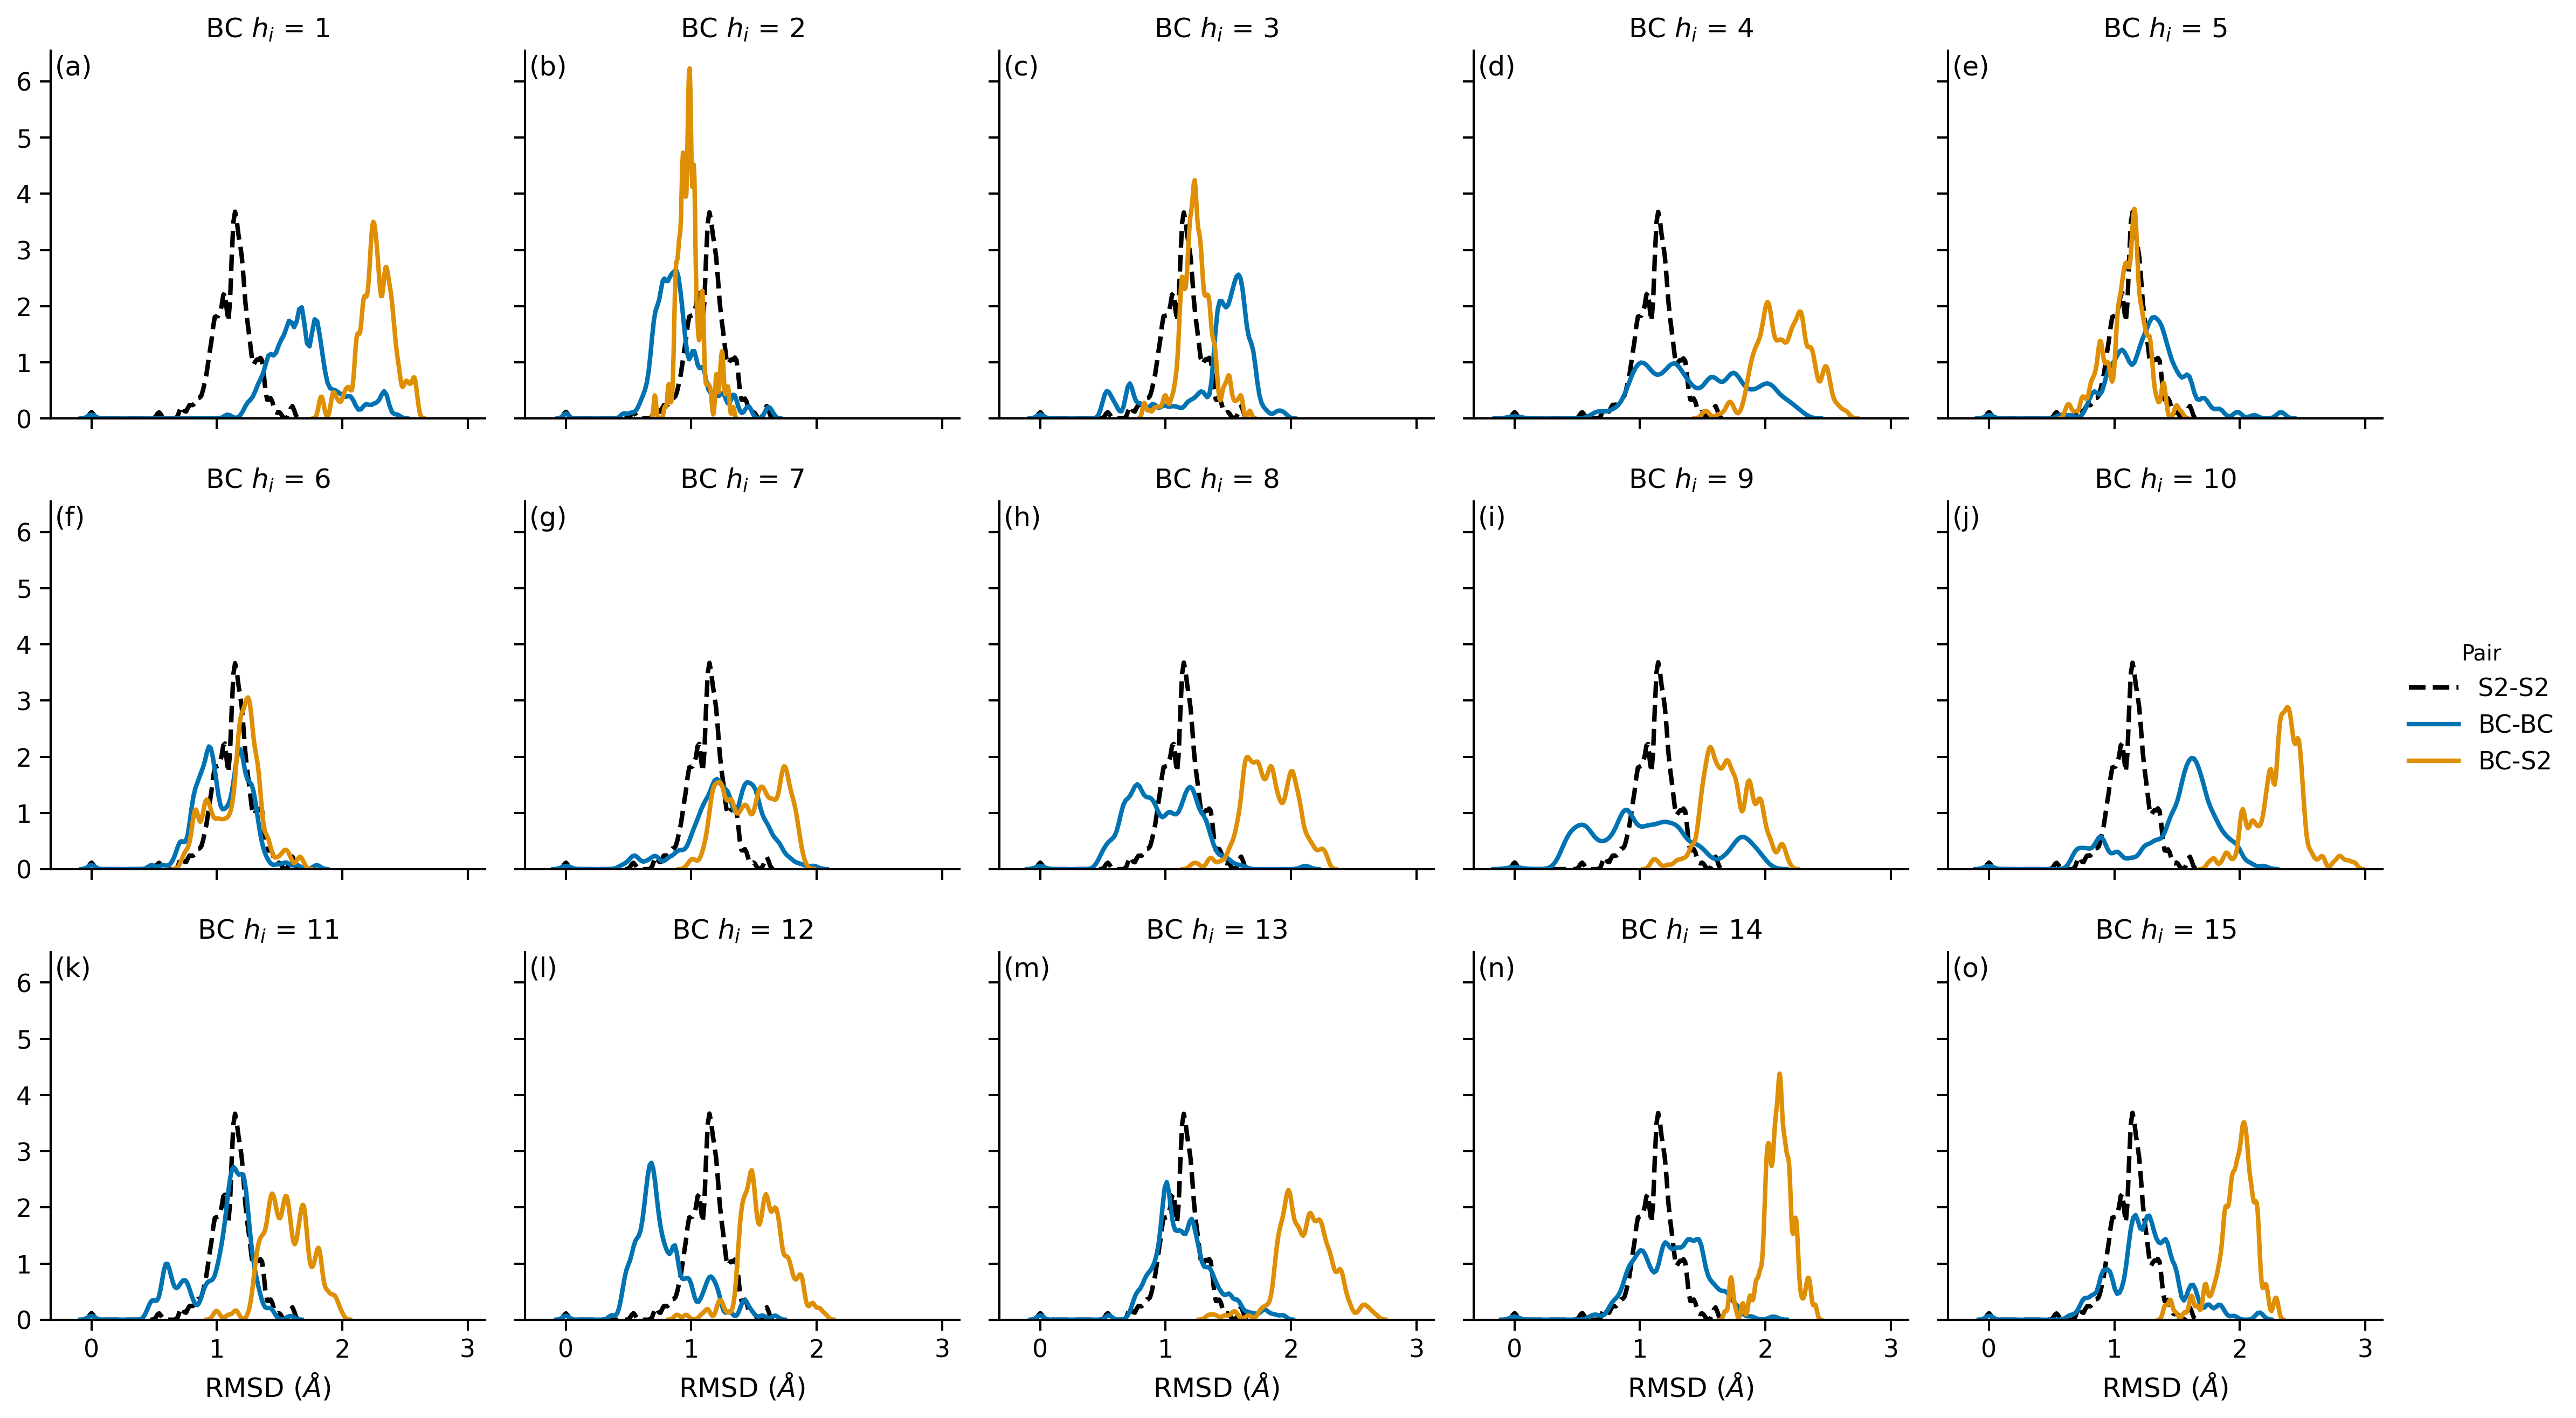
\includegraphics[width=0.8\textwidth]{chapters/aadh/figures/sensitivity_2_5_overlap.png}
\end{figure}




